\documentclass[a4paper, twoside, titlepage]{book}

\usepackage[T1]{fontenc}
\usepackage[utf8]{inputenc}
\usepackage[italian]{babel}

\usepackage{microtype}
\usepackage{xcolor}
\usepackage{titlesec}
\usepackage{xargs}
\usepackage{multicol}
\usepackage{amsmath}
\usepackage{amssymb}
\usepackage{quoting}
\quotingsetup{font=small}

\usepackage{pdfpages}

\usepackage{verse} % utilizzo dell'ambiente per la scrittura in versi
%modifica la posizione del numero di verso
\setlength{\vrightskip}{-30pt}%regola tu
 \verselinenumbersleft
%

\usepackage{ulem}
\usepackage{framed}
\usepackage{amsmath}
\usepackage{graphicx}

\DeclareUnicodeCharacter{200B}{{\hskip 0pt}}

%creazione del comando per le note a margine
\newcounter{mar}
\newcommand{\mar}[2]{
\addtocounter{mar}{1}
\hspace{-0.73em}\textsuperscript{\hyperref[\thechapter.\themar]{\themar}}\marginpar{{\small\textbf{\themar}\label{\thechapter.\themar}. #2}}\hspace{-0.4em}
}
\newcommand{\mat}[1]{\mar{gg}{#1}}
%fine comando per le note a margine

%definizioni particolari
\newcommand{\straniero}[1]{\textit{#1}} %parole straniere
\newcommand{\titolo}[1]{\textsc{#1}} %titoli
\newcommand{\evid}[1]{\textbf{\textcolor{blue}{#1}}} %parole evidenziate
\newcommand{\salt}{\hspace{1em}[...]} %comando per la creazione dei puntini di sospensione tra quadre
\newcommand{\elenco}[1]{%
\begin{itemize}
#1
\end{itemize}}
\newcommand{\elencon}[1]{%
\begin{enumerate}
#1
\end{enumerate}}
%

%citazioni
\newcommand{\citazione}[1]{%
  \begin{quotation}
  \noindent #1
  \end{quotation}}
%

%definire header e footer
\usepackage{fancyhdr}
\pagestyle{fancy}

\fancyhf{}
\fancyhead[LE,RO]{\scshape\thepage}
\fancyhead[LO]{\scshape\footnotesize\nouppercase{\rightmark}}
\fancyhead[RE]{\scshape\footnotesize\nouppercase{\leftmark}}
%

%rimuovere header e footer dalle pagine vuote
\makeatletter
\def\cleardoublepage{\clearpage\if@twoside \ifodd\c@page\else
    \hbox{}
    \vspace*{\fill}
    \vspace{\fill}
    \thispagestyle{empty}
    \newpage
    \if@twocolumn\hbox{}\newpage\fi\fi\fi}
\makeatother
%

\renewcommand{\emph}[1]{\textcolor{blue}{#1}}

%%%%%% HYPERREF VA CARICATO SEMPRE PER ULTIMO, DEMENTE!

\usepackage[colorlinks, pdftex, pdfauthor={Davide Peccioli},
            pdftitle={Appunti Letteratura},
            pdfsubject={Svevo, Pirandello e Nietzsche}]{hyperref}
\definecolor{RoyalBlue}{rgb}{0.0, 0.14, 0.4}
\hypersetup{
     colorlinks=true,
     linkcolor=blue,
     filecolor=blue,
     citecolor = black,
     urlcolor=cyan,}

\begin{document}

\begin{titlepage} % pagina del titolo
\begin{center}
    \null
    \vfill
    {\huge \textsc{Appunti di Letteratura}}\\
    \vspace{2em}
    {\Large Pascoli, Svevo e Pirandello}\\
    \vspace{3em}
    {\large \textbf{Davide Peccioli}}\\
    \vspace{1em}
    {\large Classe 5\textsuperscript{a}\\\vspace{0.4em} 21 maggio 2021}
    \fancyfoot[C]{}
    \vfill
\end{center}
\end{titlepage}
\tableofcontents

\part{Pascoli}

\chapter{Introduzione e caratteri generali}

Pascoli è passato alla storia come il poeta delle piccole cose: in Pascoli abbiamo molte poesie, brevi, graziose, sembrano dei bozzettini impressionistici con immagini di campagnia, e quindi talvolta i termini possono apparire semplici.
Aveva una vera e propria passione per la botanica: abbiamo una serie di immagini e nomi di fiori, scene di campagna e della natura.

L'immagine di Pascoli come poeta delle piccole cose è piuttosto vecchia, e in tempi recenti è stata parecchio modificata, riconsegnandoi un Pascoli decisamente più interessante: le piccole cose che molto spesso troviamo nelle sue poesie sono \textbf{simboli}; Pascoli sembra essere giunto in modo autonomo a quelle soluzioni tipiche della poesia simbolista che si stavano sviluppando in Europa, soprattutto nella letteratura francese.

Tutte le scelte foniche, linguistiche, sintattiche e lessicali di Pascoli rimandano a qualcosa \textbf{d'altro}: conoscendo la personalità di Pascoli, la sua sintassi frantumata, i suoi suoni onomatopeici (figure retoriche apparentemente comunissime), spesso rimandano a qualcos'altro di molto più profondo:
\elenco{\item la \textbf{sintassi frantumata} rimanda ad un mondo che non trova più un ordine: i poeti non si ritrovano più, non si riconoscono più nella realtà che li circonda, e a tutto questo si aggiunge il vissuto personale di Pascoli, che specie nell'ultima parte della sua vita è afflitto da timori}
Pascoli quindi non è più visto come il poeta delle piccole cose: indubbiamente sono quelli gli strumenti che egli utilizza, ma al giorno d'oggi egli è visto come un poeta dalla psicologia non disturbata, ma sicuramente particolare: queste situazioni estreme consentono di avere una sensibilità tale da cogliere i segnali dal mondo.

In Pascoli, il poeta si identifica con il \textbf{fanciullino}, il poeta è colui che ha mantenuto quel tipo di atteggiamento un po' ingenuo nei confronti della realtà, con quella sensibilità distintiva tipica del bambino, che è in grado di cogliere quei segni della natura, quei segni sotterranei nascosti: attraverso la poesia Pascoli li restituisce al lettore.

La figura retorica dell'\textbf{analogia} diventa dominante: l'analogia funziona come accostamento tra due elementi, ma è un accostamento che non si basa più su nulla di esplicito: vengono accostati elementi distantissimi tra di loro, e questo accostamento inaspettato inusuale colpisce più profondamente.
L'analogia diventa una figura dominante, così come avviene in generale nella poesia simbolista


\section{Biografia}

Nasce nel 1855, in Romagna, in una famiglia appartenente ad una borghesia media benestante: molto patriarcale e numerosa. Il padre era fattore della tenuta dei Principi Tolonia.

Egli poteva permettersi il mantenimento più che onorevole di questa numerosa famiglia.
Fin da piccolissimo Pascoli entra a studiare in collegio, come i suoi fratelli.

Nel 1867 muore il padre, avvenuta attraverso omicidio: il 10 agosto del 1867, il padre di Pascoli viene ucciso a fucilate. Fu sconvolgente per la famiglia: omicidio crudele fatto per gelosia; la famiglia conosceva i mandanti.

La giustizia non giunse mai a nessuna conclusione: questo fu molto straziante per il poeta; non era soltanto la perdita del padre, ma anche il senso di profonda ingiustizia che il poeta vive in età molto tenera; questo diventa il tema dominante di quasi tutte le sue poesie, nonché ragione di una crescita psicologia particolare del poeta. La psiche del poeta si è fermata in quell'anno, a 12 anni.
Non a caso Pascoli, parlando della sua poetica, parlerà del \textbf{fanciullino}

Il fanciullino è colui che guarda la realtà con gli occhi del bambino, e riesce a cogliere degli elementi che fuggono all'adulto.

Le conseguenze di questo episodio sono vissute anche a livello economico: l'anno successivo alla morte del padre, con una frequenza spaventosa, inizieranno a morire molti altri elementi della famiglia: nei tre anni successivi la madre, la sorella, e altri fratelli, tra cui Luigi e il fratello più grande, che aveva preso le redini finanziarie.
Questo porta ad un altro tema della sua poesia, ovvero le difficoltà economiche: riuscì a studiare solo grazie a borse di studio e alla benevolenza dei suoi professori, che riconoscevano le doti di questo scrittore.

Divenne classicista e grechista, e ottenne la cattedra che era stata di Carducci. Partecipò a molti concorsi di poesia in lingue antiche.

Nella sua vita non capita quasi nulla, se non un episodio in età giovanile, quando studiava all'università a Bologna, nel 1879: Pascoli si avvicina alla vita politica militante: come giovane studente universitario si avvicina al socialismo ed inizia a partecipare ad alcune manifestazioni; ad una di queste viene catturato, e fece alcuni mesi di carcere. Questa fu una esperienza fu per lui traumatica, tanto che abbandonò la politica militante per sempre, ritirandosi in una vita in campagna, lontano dai riflettori.

Egli amava tantissimo la campagna, i fiori, nonché i riti della campagna; si racconta che amava frequentare i contadini, verso sera si ritirava molto spesso con loro a bere, giocando a carte. La sua dimensione ideale era quella della campagna.


\section{T: \textit{Biglietto per Ida}}

\begin{figure}
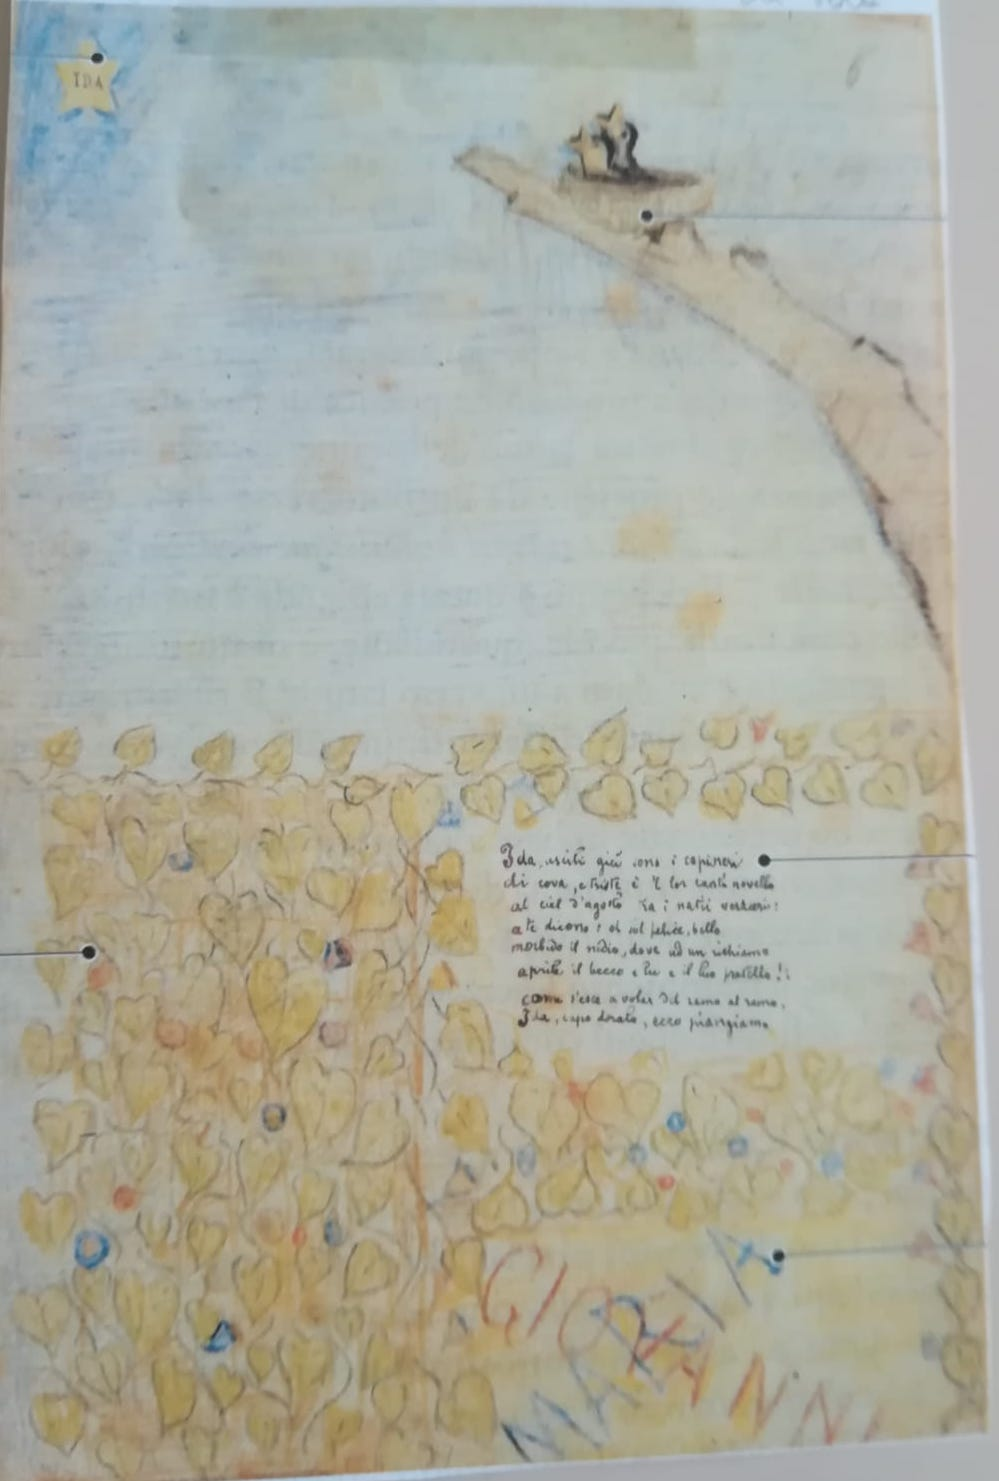
\includegraphics[width=\textwidth]{1}
\caption{\textit{Biglietto per Ida}}
\end{figure}

Vediamo sotto i nomi dei due fratelli, Giovanni e Mariù, incrociati sul fondo.
Attorno alla scritta ci sono foglie e cuori.
In alto c'è una stella, che è Ida (che si stava sposando).
C'è un nido con due uccellini che piangono, che rappresentano lui e la sorella Maria.

Gli unici fratelli che sono rimasti uniti fra di loro sono Giovanni, Maria e Ida.
È un nucleo famigliare che ha rifiutato la possibilità, dopo la tragedia dell'infanzia, di ricostruire una nuova famiglia, ma anzi ha sempre cercato di ricostruire quel nucleo finito molto tempo addietro.

Quando Ida si sposa, i due fratelli, che hanno un rapporto quasi morboso e inquietante, che ritorna prepotentemente nelle poesie, per gli altri due è come se nuovamente fosse venuto qualcosa a distruggere quel nido famigliare.

Pascoli ha avuto la possibilità di sposare una cugina, ma la reazione di Mariù è così terribile da farlo desistere. I carteggi tra Giovanni e la fidanzata hanno del terribile.

\section{Temi}

Sono tutti comportamenti anomali che ci mostrano lo stato psicologico di questo poeta.

Egli è quasi l'unico poeta che non ha scritto poesie d'amore. La tematica dell'amore, che è la più frequente in poesia, è trattato molto poco, e viene sempre visto come qualcosa di misterioso e torbido.

Questo deve essere una chiave di lettura per la poesia di Pascoli: non troviamo una ideologia politica, ma è \textbf{poesia pura}, con un grande uso degli aspetti musicali e fonici.

Con Pascoli abbiamo soluzioni pari a quelle del simbolismo francese, a cui il poeta giunge attraverso soluzioni personali.

Risulta molto difficile, di fronte ad un testo poetico, rispondere alla domanda "di cosa parla?"

Alcuni temi ricorrenti sono il \textbf{nido}, che rappresenta la famiglia che è stata distrutta, e che lui cerca di ricostruire in maniera \textit{non naturale}, in quanto cerca di farlo con gli stessi elementi del passato. Le sorelle diventano figure materne, e lui è un fanciullino di 12 anni.

Il tema della \textbf{morte} è onnipresente nella poesia di Pascoli. Si presenta con delle suggestioni che il poeta coglie e cerca di trasmetterci

Nella poesia di Pascoli è assente una parte filosofia espressa, come avveniva per Leopardi: è tutto lasciato a suggestioni, immagini e suoni.


\section{Pascoli e il positivismo}

Cronologicamente gli anni in cui Pascoli si forma sono gli anni del positivismo (anni '70), e del resto vediamo la sua mania di usare i termini scientifici per appellarsi ai fiori.

Per certi aspetti quindi Pascoli si colloca ancora in questo clima. Allo stesso tempo fa parte di questo clima decadente che caratterizza la fine del secolo.

\chapter{\textit{Myricae}}
\elenco{\item \emph{p. 553}}

Myricae è un termine latino, che significa tamerici (un arbusto).

È una raccolta poetica di Pascoli, iniziata nel 1891. All'inizio ci sono pochissimi testi, ma nelle edizioni successive vengono aggiunti nuovi componimenti: nell'edizione definitiva ci sono più di 100 componimenti.

È forse la raccolta di poesie più famosa di Pascoli.

Il titolo è una citazione di Virgilio, colta dal poeta con il significato contrario rispetto al termine usato da Virgilio.
Virgilio dice che non a tutti piacciono le myricae (ovvero le piante semplici), e che quindi per venire incontro a tutti lui avrebbe innalzato lo stile.
Pascoli ne fa il titolo della sua opera: indica con questo titolo che le sue poesie sono cose semplici (e per questo a lungo Pascoli era stato preso come il poeta delle piccole cose). La forza di queste poesie è però nel loro significato simbolico

\section{T: \textit{Arano}}

Il soggetto del titolo è "i contadini". In Pascoli il titolo diventa un elemento fondamentale per capire la poesia.
Abbiamo un paesaggio di campagna.
Non è un sonetto, è formato da due terzine e una quartina.

Nei primi quattro versi è creata un'immagine

\begin{verse}
\poemlines{5}
Al campo\mat{senso di vago e indefinito}, dove roggio nel filare\\
qualche pampano\mat{foglie della vite} brilla, e dalle fratte\\
sembra la nebbia mattinal\mat{cortina, senso di protezione; vago e indefinito} fumare,\\!
arano\mat{senza soggetto, dopo quattro versi}: a lente grida, uno le lente\\
vacche spinge; altri semina; un ribatte\\
le porche con sua marra pazïente;\mat{ipallage che rimanda alla pazienza (\textit{sopportare})}\\!
chè il passero saputo\mat{cambia la prospettiva} in cor già gode,\\
e il tutto spia dai rami irti del moro;\\
e il pettirosso:\mat{punteggiatura forte} nelle siepi s’ode\\
il suo sottil tintinno come d’oro.\mat{onomatopea}
\end{verse}

Il primo verbo, (\textit{arano}, \textbf{v. 4}) crea un senso di lentezza e di sospensione, in quanto compare dopo ben quattro versi: vi è il senso della fatica del lavoro, rimarcato da tutta la seconda strofa.
La campagna per Pascoli è intesa positivamente, diversamente da
quello che accade in Verga, ma è innegabile la fatica del lavoro, che
diventa fatica della vita. Questo emerge dal ritmo della poesia

Il passero è \textit{saputo} (\textbf{v. 7}): ci rimaanda immediatamente al \titolo{Passero Solitario} di Leopardi. Il passero è esperto perché non migra e aspetta e spia il lavoro dell’uomo e sa che troverà del cibo per l’inverno.

È presente un simbolo di punteggiatura forte (\colorbox{yellow}{:}, \textbf{v. 9}); le regole formali di Pascoli sembrano piuttosto canoniche,
ma in realtà lui le “distrugge da dentro”, con separazioni
dettate da questa punteggiatura, parentesi, enjambements;
tutti elementi che richiamano alla solitudine, allo strappo, alla
separazione.

Sono molto presenti gli enjambement, che spezza e unisce allo stesso tempo. Si allunga il tempo della lettura: crea una attenzione particolare del lettore rispetto ai termini in questione.
Siccome si tratta di una spezzatura, in Pascoli molto spesso provoca e va a sostenere il senso di solitudine, di essere separato e strappato.

Fa parte di una sezione che si intitola “ultima passeggiata”, in cui lascia tutta una serie di poesie, piccoli bozzetti: rimandano ad una concezione realistica e coloristica, al punto che si definiscono quasi “impressionistiche”
Il paesaggio assume un significato simbolico.
Questi sono paesaggi che il poeta vede prima di recarsi in città.
Questo pendolarismo è effettivamente nella sua biografia

Pascoli ha ben presente la lezione di Esiodo: lo lesse, e in questa poesia ci trasmette la \textbf{fatica del lavoro}, tema molto presente in Esiodo.

Ciò che il poeta ci vuole trasmettere lo percepiamo in parte da ciò che ci dice, ma soprattutto lo percepiamo dall’uso di alcune forme retoriche, all’uso di termini che rimandano a colori.

\begin{center}
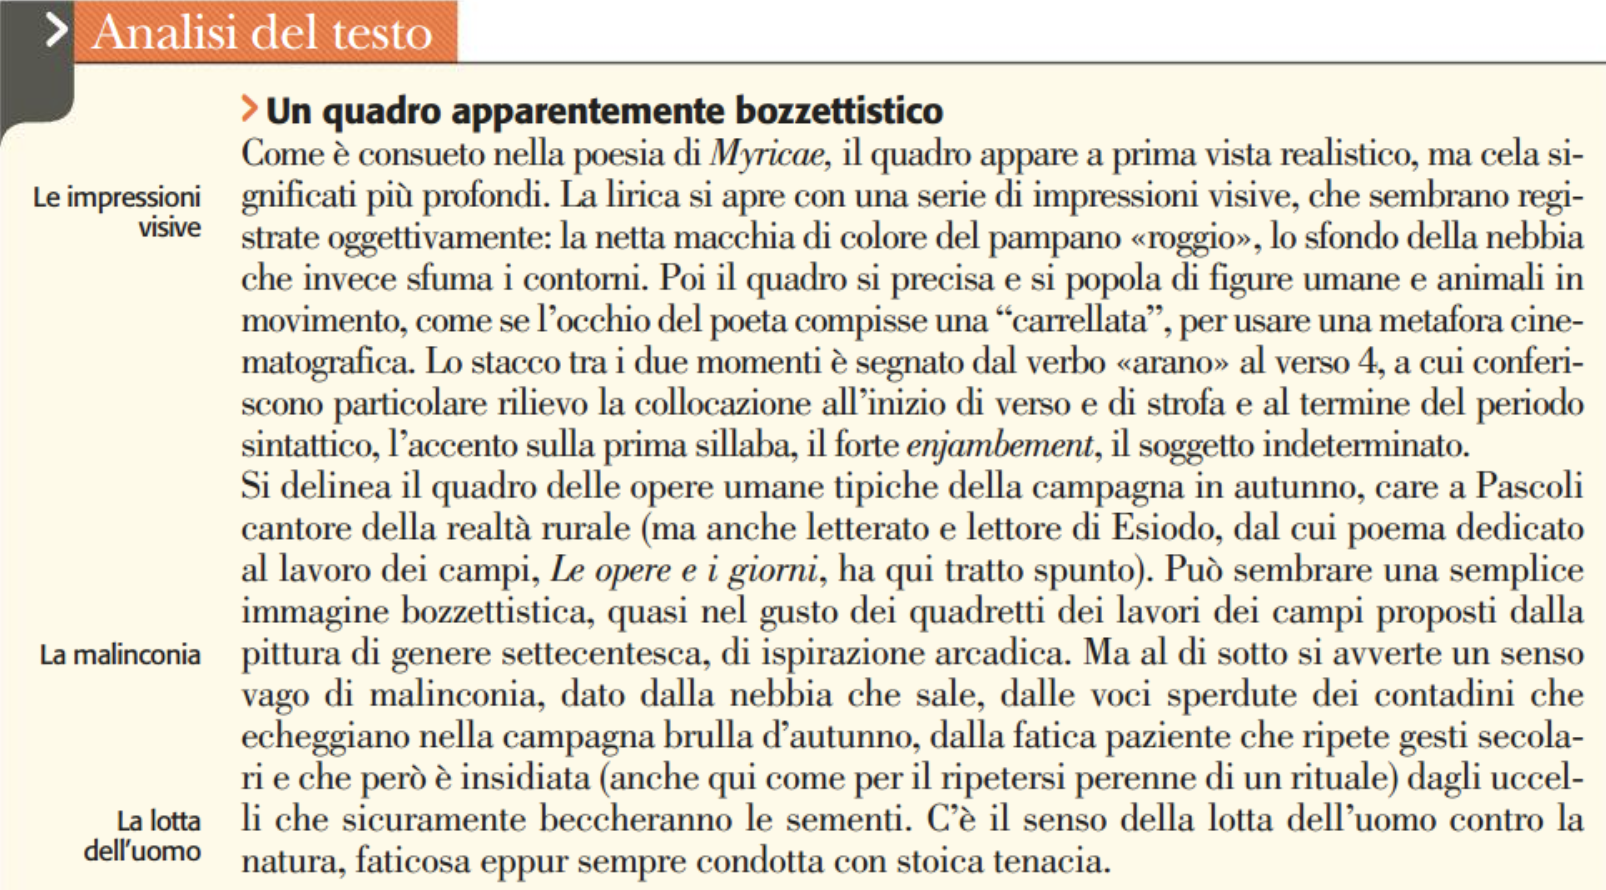
\includegraphics[width=\textwidth]{arano1}
\end{center}

\begin{center}
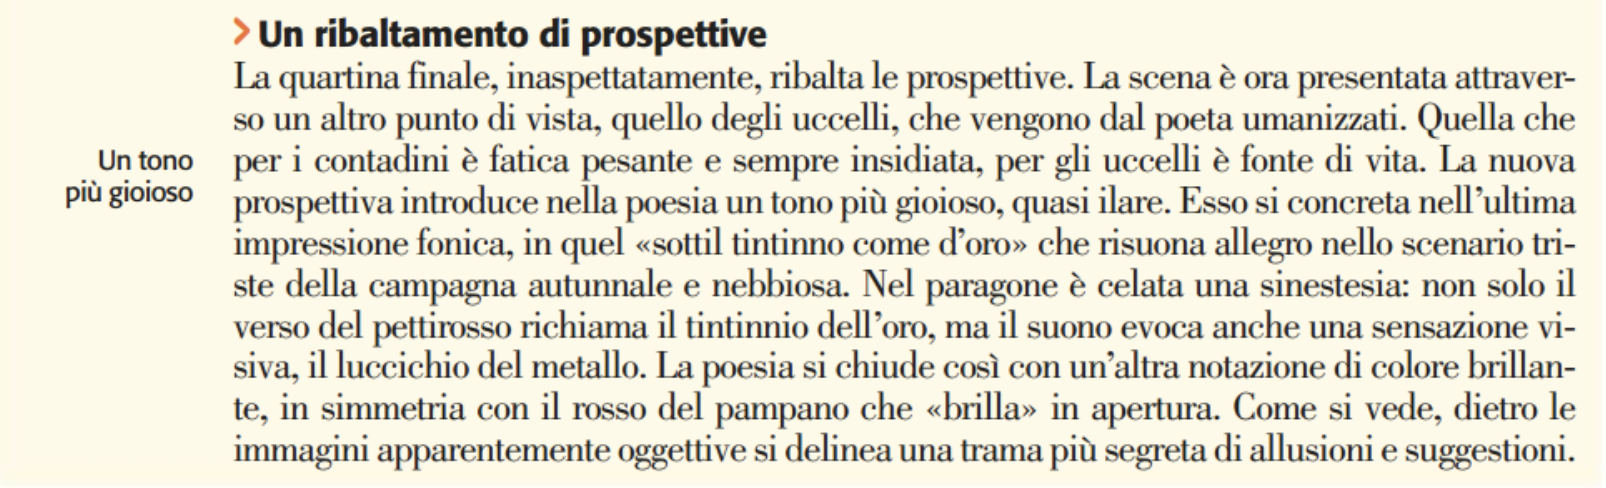
\includegraphics[width=\textwidth]{arano2}
\end{center}

\section{T: \textit{Lavandare}}

Questa poesia fa sempre parte della sezione “l’ultima passeggiata”, e l’Io lirico passeggiando sente il canto delle lavandaie.
Nella seconda parte della poesia sono riportati dei versi di alcune canzoni popolari realmente esistenti, che si ricollegano al tema del suono già presente nella prima parte della poesia.

\setcounter{mar}{0}
\begin{verse}
Nel campo mezzo\mat{a metà} grigio e mezzo nero\\
resta un aratro senza buoi, che pare\mat{tutto indica solitudine e abbandono, compreso l'enjambement}\\
dimenticato, tra il vapor leggero.\\!
E cadenzato dalla gora viene\\
lo sciabordare\mat{onomatopeico: nella poesia di Pascoli è importante la componente sonora} delle lavandare\\
con tonfi spessi\mat{non parafrasabile: due figure retoriche, sinestesia e onomatopea} e lunghe cantilene:\\!
Il vento soffia e nevica\mat{non è un verbo transitivo, ma è usato come tale} la frasca,\\
e tu\mat{a capo, come sospeso} non torni ancora al tuo paese!\\
quando partisti, come son rimasta!\\
come l’aratro\mat{l'aratro è abbandonato } in mezzo alla maggese.
\end{verse}

Questa poesia comunica un senso di abbandono e di solitudine. La poesia non ha un significato, un concetto, un tema: non vuole comunicare una idea.
Lo stesso pascoli diceva che la poesia non serviva a niente, non aveva finalità. La finalità sbucava fuori da sola: proprio per essere priva di finalità essa è apprezzabile solo per il piacere che può comunicare; la finalità diventa quindi quella di creare qualcosa di bello per l’uomo.

Gli ultimi tre versi sono parte di una canzone popolare.

\begin{center}
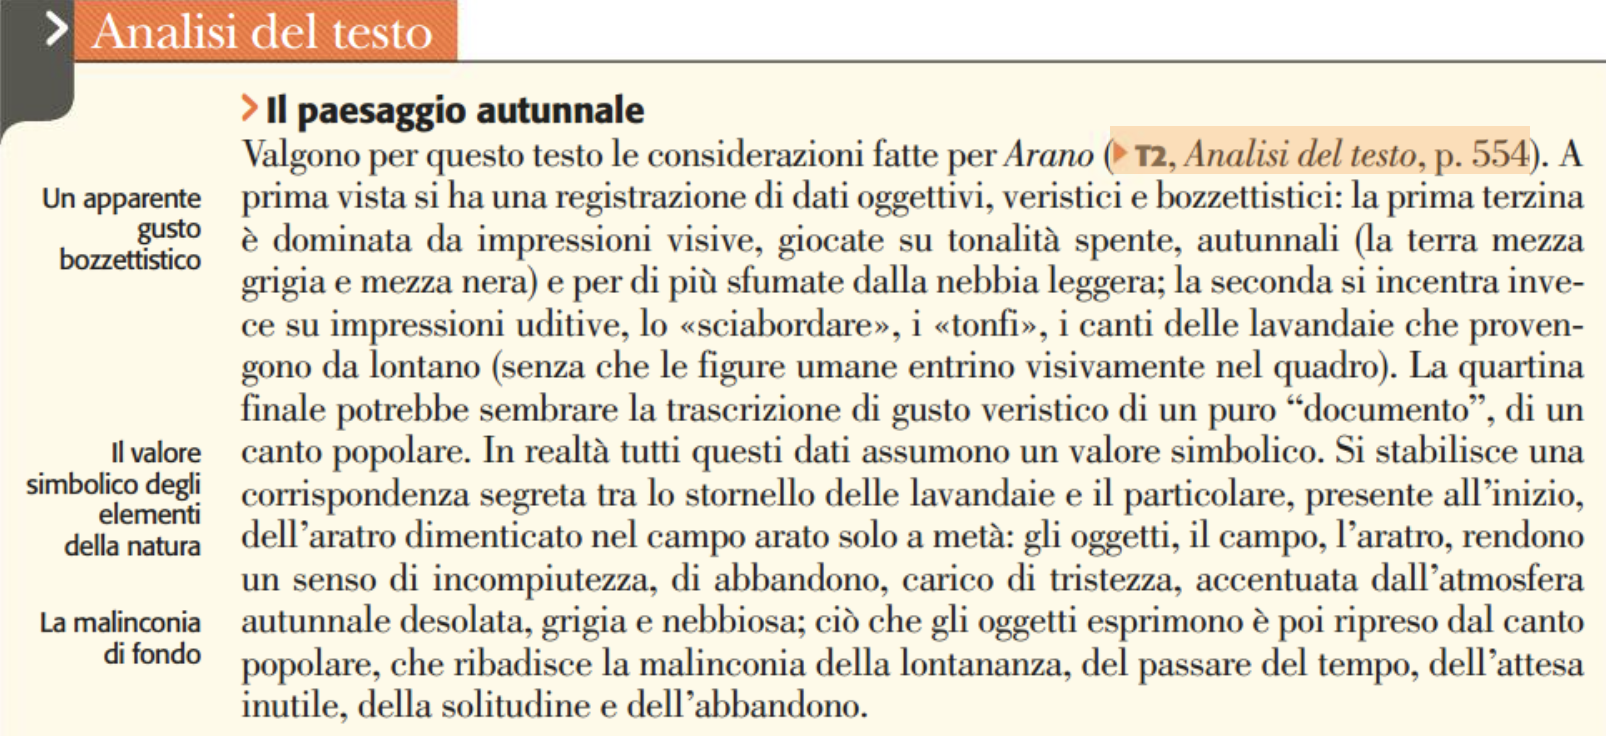
\includegraphics[width=\textwidth]{lavandare1}
\end{center}

\begin{center}
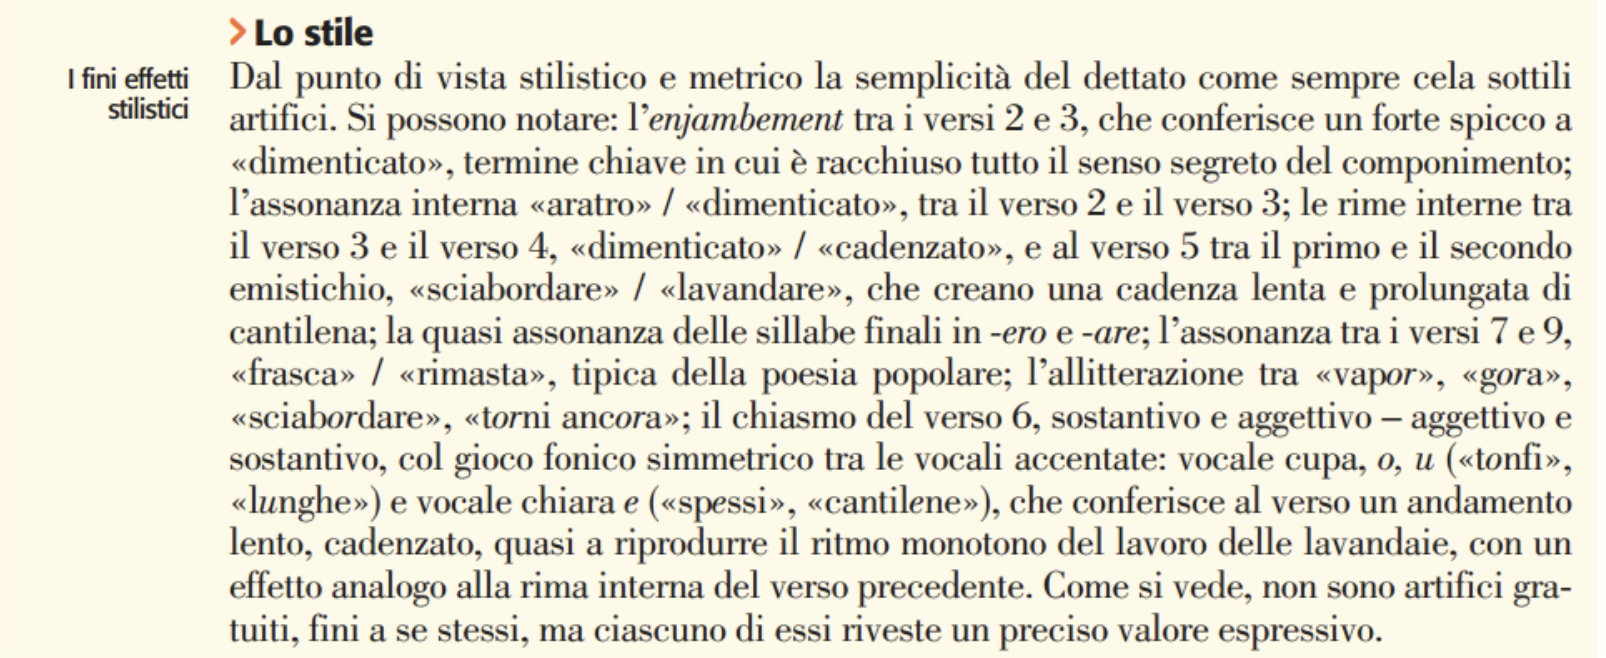
\includegraphics[width=\textwidth]{lavandare2}
\end{center}

\section{T: \textit{X agosto}}

Giorno della morte del padre.
Quando il padre venne colpito dalla fucilate, la cavalla che lo portava giunse comunque a casa (portando il cadavere).
C’è una poesia in cui Pascoli immagina la madre interrogare la cavalla a riguardo dell’omicidio.

Il 10 agosto è anche il giorno di San Lorenzo, in cui ci sono le stelle cadenti, che esprimono i desideri.
Pascoli interpreta questo suo dolore personale, questo suo lutto, come un lutto che investe tutta l’umanità: quindi interpreta le stelle cadenti come le lacrime del cielo

\begin{verse}
San Lorenzo, io lo so perchè tanto\\
di stelle per l’aria tranquilla\\
arde e cade, perchè sì gran pianto\\
nel concavo cielo sfavilla.\\!
Ritornava una rondine\mat{padre di Pascoli} al tetto\mat{sia metafora che sineddoché: la confuzione tra nido e casa è voluta}:\\
l’uccisero: cadde tra spini\mat{corona di spine di Cristo: quasi come se il padre diventasse una vittima sacrificale, giustifica il dolore del mondo}:\\
ella aveva nel becco un insetto:\\
la cena de’ suoi rondinini\mat{familiari di Pascoli}.\\!
Ora è là, come in croce\mat{altra allusione a Cristo}, che tende\\
quel verme a quel cielo lontano;\\
e il suo nido è nell’ombra\mat{vago e indefinito: l'oscurità ha valore negativo}, che attende,\\
che pigola sempre più piano.\\!
Anche un uomo tornava al suo nido:\\
l’uccisero: disse: Perdono;\\
e restò negli aperti occhi un grido:\\
portava due bambole, in dono...\mat{In questa strofa l'analogia diventa esplicita: la rondine va a casa e l'uomo va al nido (inteso non solo come cassa ma anche come prole, metonimia)}\\!
Ora là, nella casa romita,\\
lo aspettano, aspettano, in vano:\\
egli immobile\mat{come la rondine}, attonito, addita\\
le bambole al cielo lontano.\\!
E tu\mat{riprende l'incipit della poesia}, Cielo, dall’alto dei mondi\\
sereni, infinito, immortale,\\
oh! d’un pianto di stelle lo inondi\mat{acqua purificatrice}\\
quest’atomo opaco del Male!\\!
\end{verse}

\begin{center}
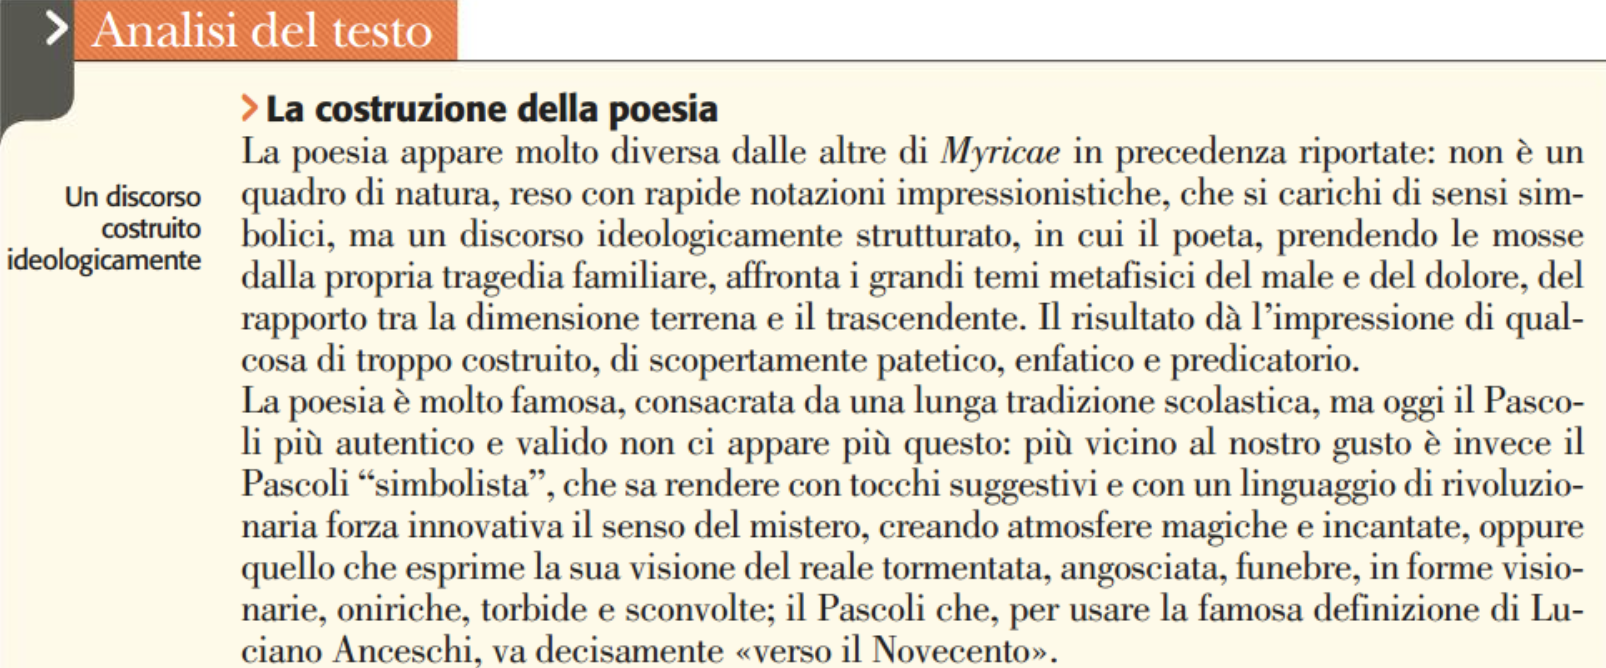
\includegraphics[width=\textwidth]{agosto1}
\end{center}

\begin{center}
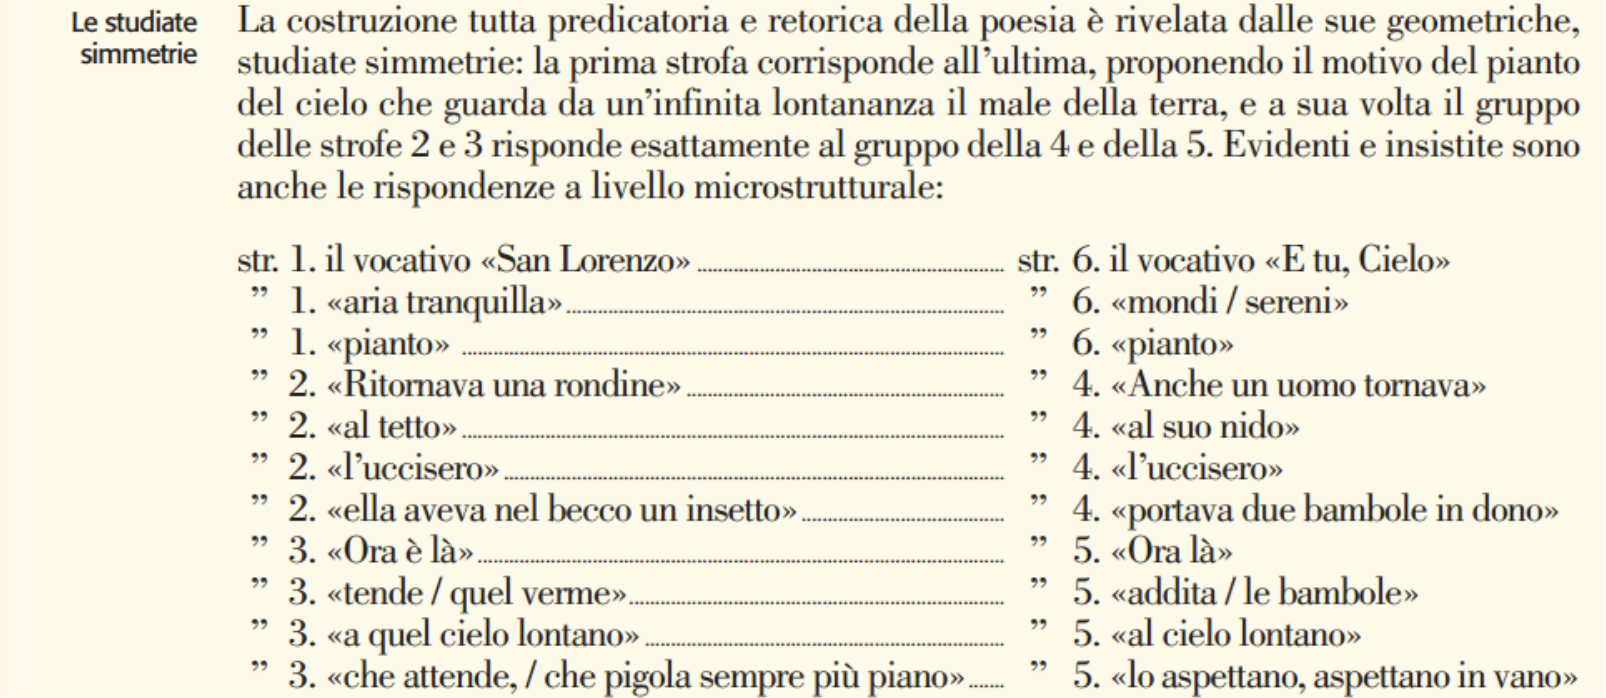
\includegraphics[width=\textwidth]{agosto2}
\end{center}

\begin{center}
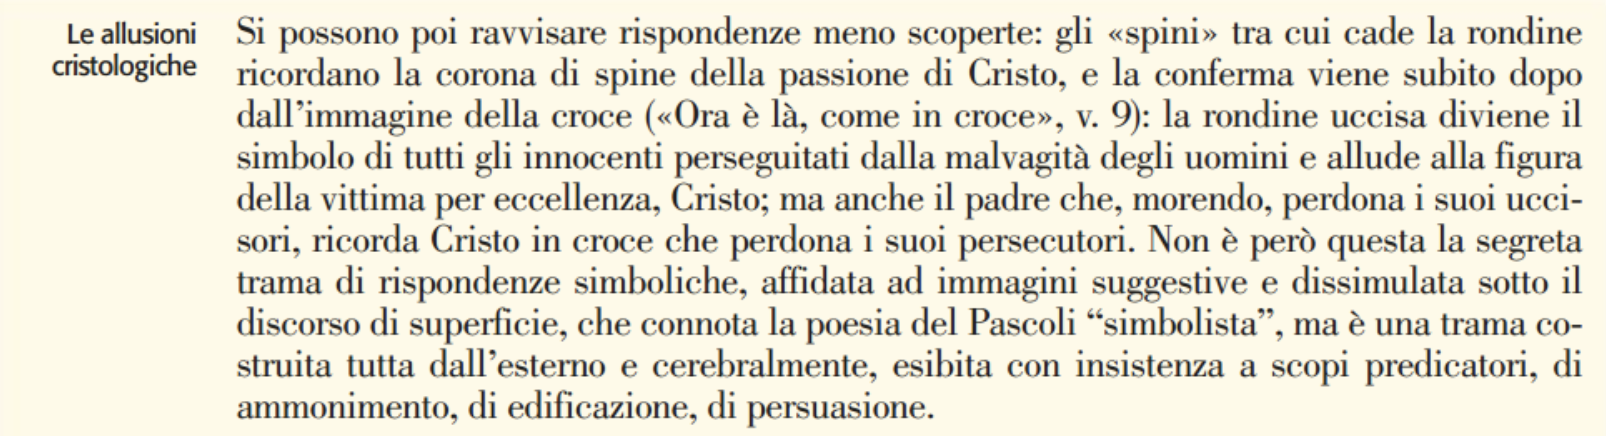
\includegraphics[width=\textwidth]{agosto3}
\end{center}

\vfill

\begin{center}
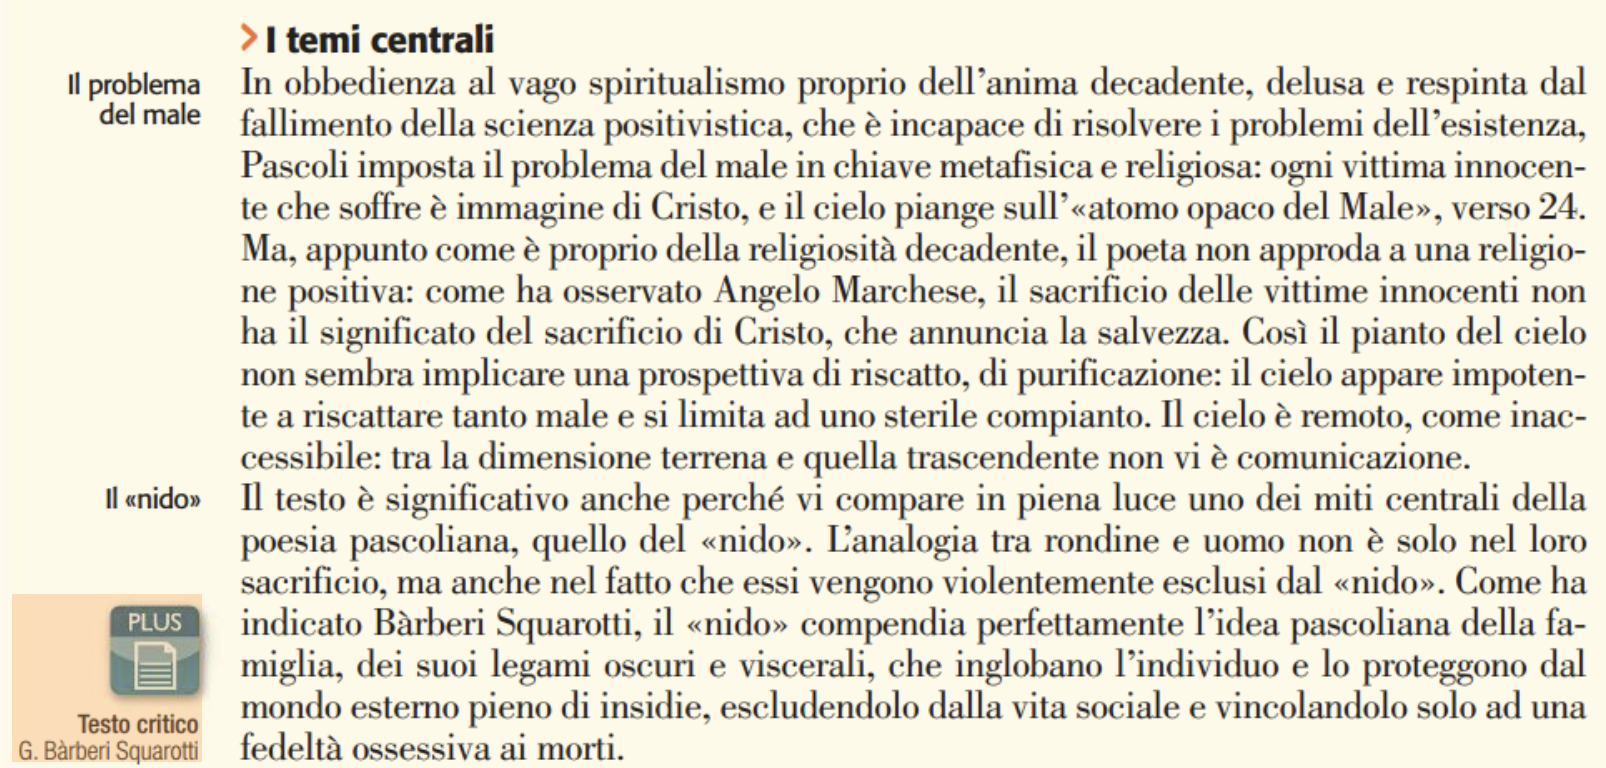
\includegraphics[width=\textwidth]{agosto4}
\end{center}

\section{T: \textit{Assiuolo}}

Il tema della morte arriva attraverso suggestioni.
La struttura è fantastica, tutto funziona alla perfezione, e le figure retoriche sono dosate in modo simmetrico.

C'è un esempio significativo dell'analogia.

Ogni strofa è organizzata secondo un sistema binario: nella prima parte c'è una immagine luminosa, e nella seconda parte una immagine lugubre, che diventa simbolo di disillusione.

\setcounter{mar}{0}
\begin{verse}
Dov’era la luna? chè\mat{causale senza reggente, senso di sospensione e attesa: aspettiamo la luce} il cielo\\
notava in un’alba di perla\mat{sta per alba chiara},\\
ed ergersi il mandorlo e il melo\\
parevano a meglio vederla\mat{attesa della luna}.\\
Venivano soffi di lampi\mat{due sostantivi, uniti dal nesso ``di''; sinestesia}\\
da un nero di nubi laggiù;\\
veniva una voce dai campi\mat{primo termine del climax, con accezione neutra, che si gioca su tutta la poesia}:\\
\textit{chiù}...\\!
Le stelle lucevano rare\\
tra mezzo alla nebbia di latte\mat{immagine molto corposa}:\\
sentivo il cullare del mare,\\
sentivo un fru fru tra le fratte\mat{allitterazione \texttt{f} e \texttt{r}: fragilità};\\
sentivo nel cuore un sussulto\mat{fa presagire il singhiozzo},\\
com’eco d’un grido\mat{grido del padre che non è mai uscito} che fu.\\
Sonava lontano il singulto\mat{secondo termine del climax}:\\
\textit{chiù}...\\!
Su tutte le lucide vette\\
tremava un \uline{sospiro di vento}:\\
squassavano\mat{movimento delle ali delle cavallette, onomatopea} le cavallette\\
finissimi sistri\mat{strumenti musicali sacri ad Iside} d’argento\\
(tintinni a invisibili porte\\
che forse non s’aprono più?...);\mat{identifica questi suoni con i suoi morti che bussano alle sue porte}\\
e c’era quel pianto di morte...\mat{terzo termine del climax}\\
\textit{chiù}...
\end{verse}

Quel \textit{alba di perla} (\textbf{v. 2}) è una analogia. L’alba qui è l’inizio della sera, cosa che ha una forte connotazione.
C’è una analogia, resa più forte dal nesso dei due sostantivi. Questa crea una immagine più forte, in quanto il sostantivo è più forte e corposo del semplice aggettivo.

L'assiuolo è un uccello notturno, e nel testo viene utilizzato il termine \textit{chiu}, come veniva chiamato in campagna; il suono riproduce il suo verso, e in campagna si pensava che questo verso portasse male.
Il suono è lugubre, ed evocano le figure dei morti. Il paesaggio è distorto dalla sensibilità del poeta

L'immagine che si ha quello di figure di morti evocate dall'ambiente lunare e notturno, che bussano cercando di mettersi in contatto con il poeta: bussano a delle porte che non si possono più aprire: non si possono mettere in contatto con il poeta.
Questa disillusione è denunciata dalle parole della poesia, dallo schema delle figure retoriche: c'è un climax che si gioca sull'interezza della poesia (con i tre termini alla fine di ogni strofa).

C'è una struttura metrica assolutamente regolare, che però attraverso forzature, sintassi usate in modo estremo, uso delle parentesi, è cambiata e distrutta. All'interno di questa struttura regolare ci sono le forzature di Pascoli, che mettono in evidenza qualcosa. La sintassi è quasi nulla, sono una serie di accostamenti senza legami.

\begin{center}
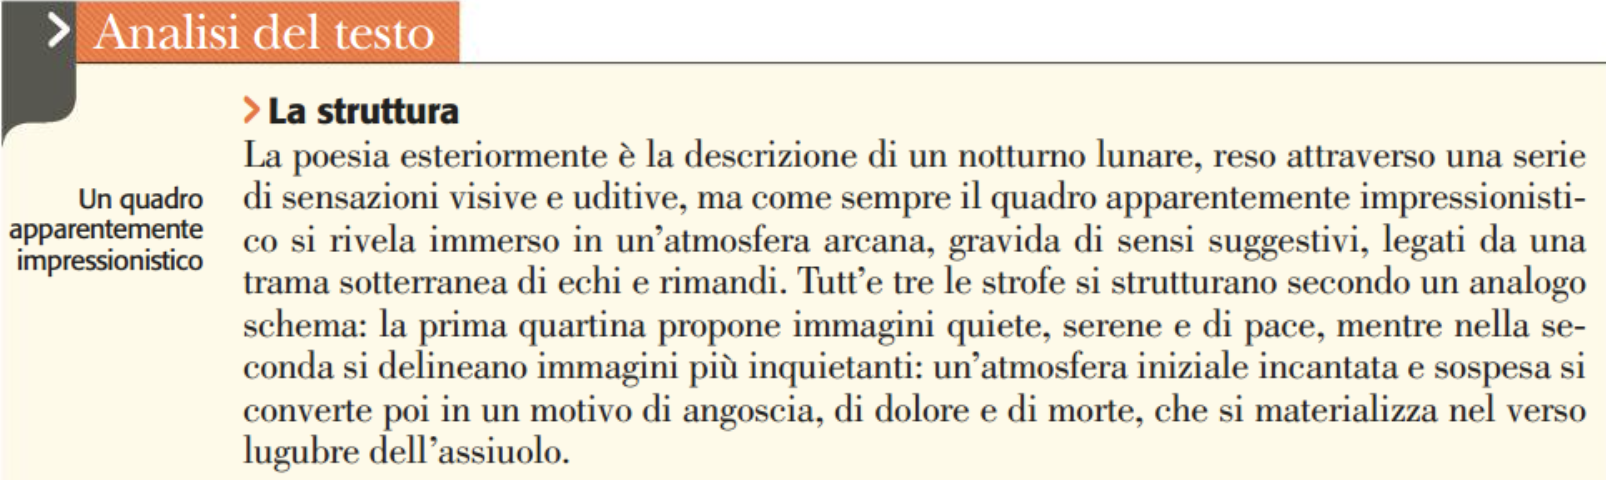
\includegraphics[width=\textwidth]{assiuolo1}
\end{center}

\begin{center}
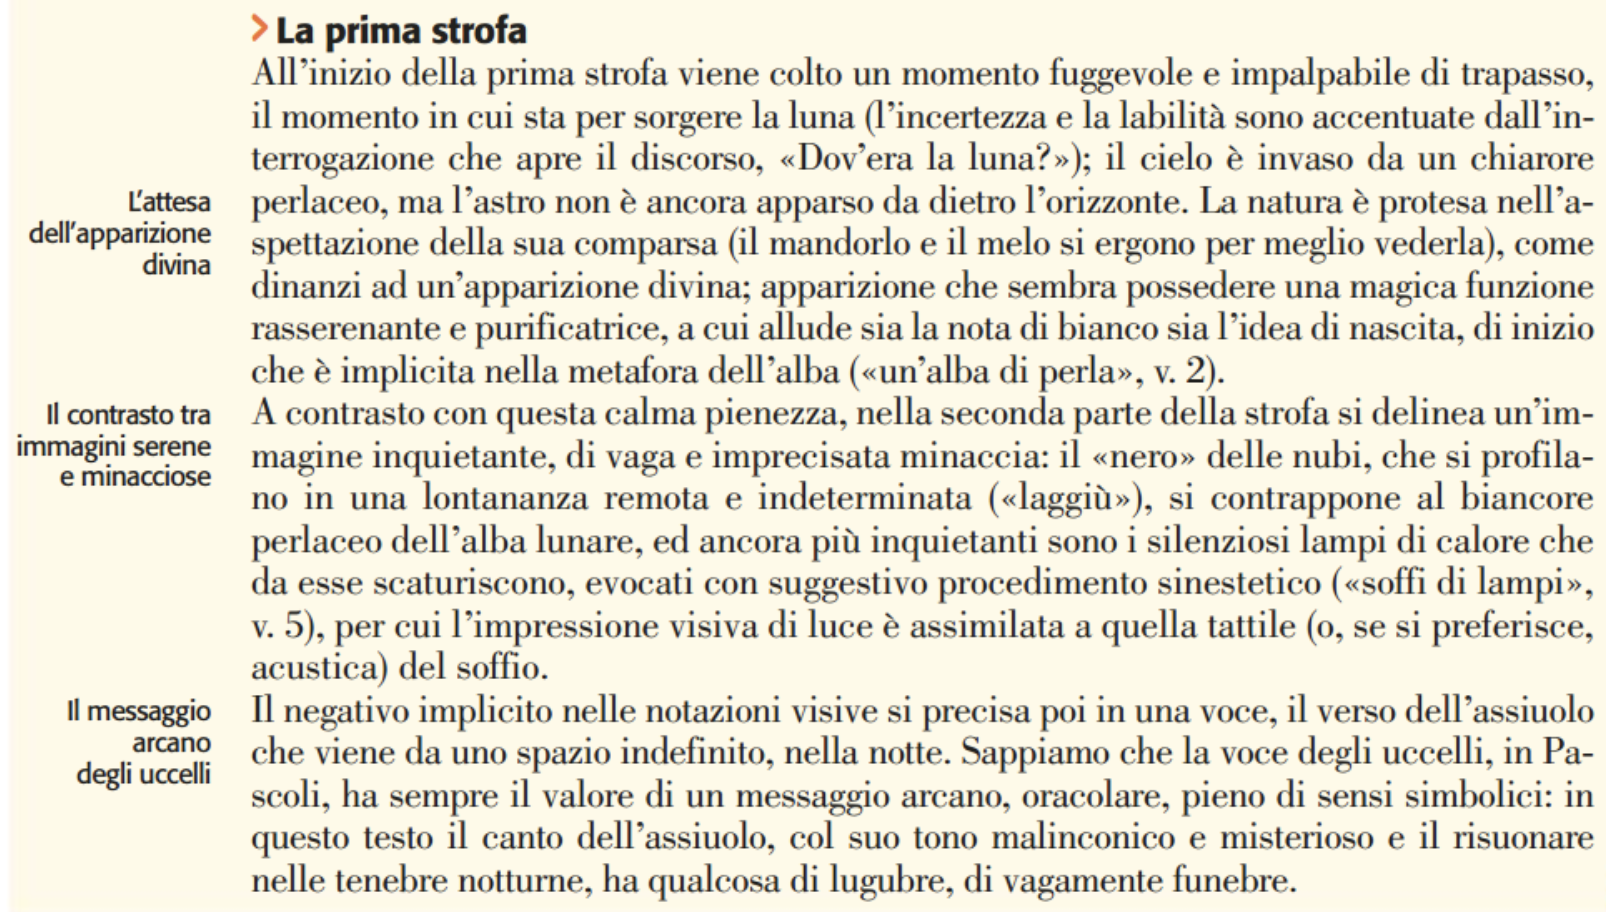
\includegraphics[width=\textwidth]{assiuolo2}
\end{center}
\vfill
\begin{center}
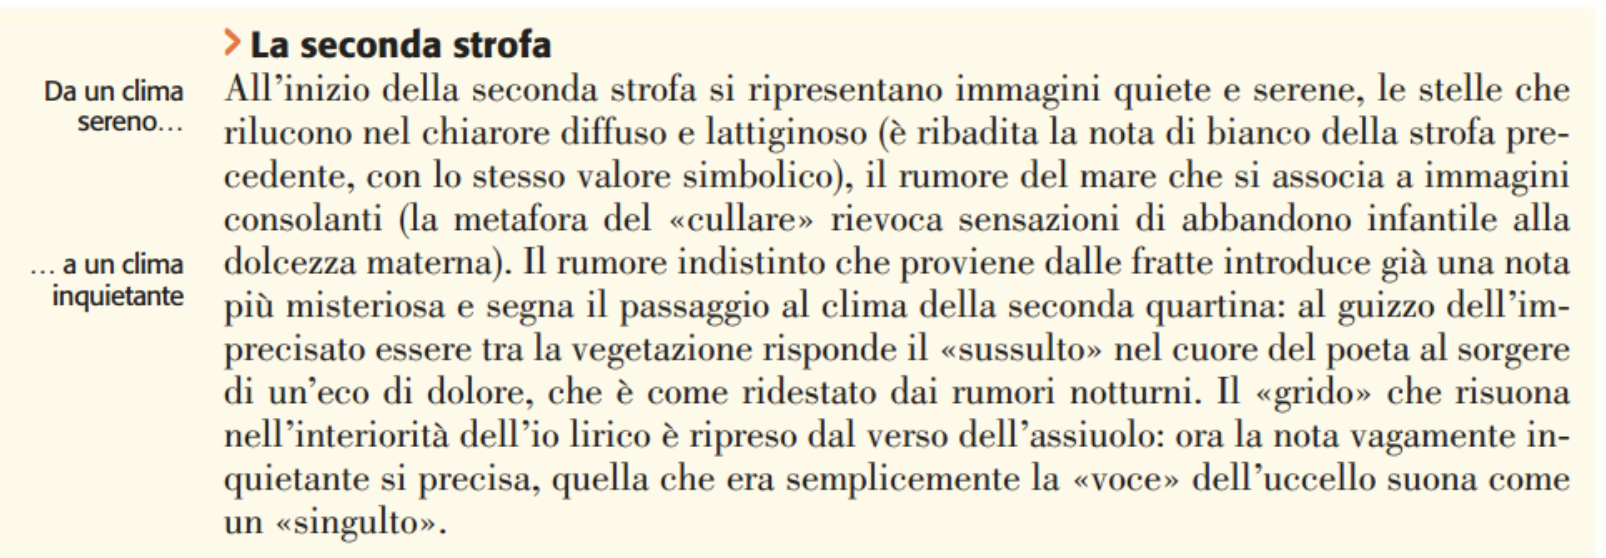
\includegraphics[width=\textwidth]{assiuolo3}
\end{center}

\begin{center}
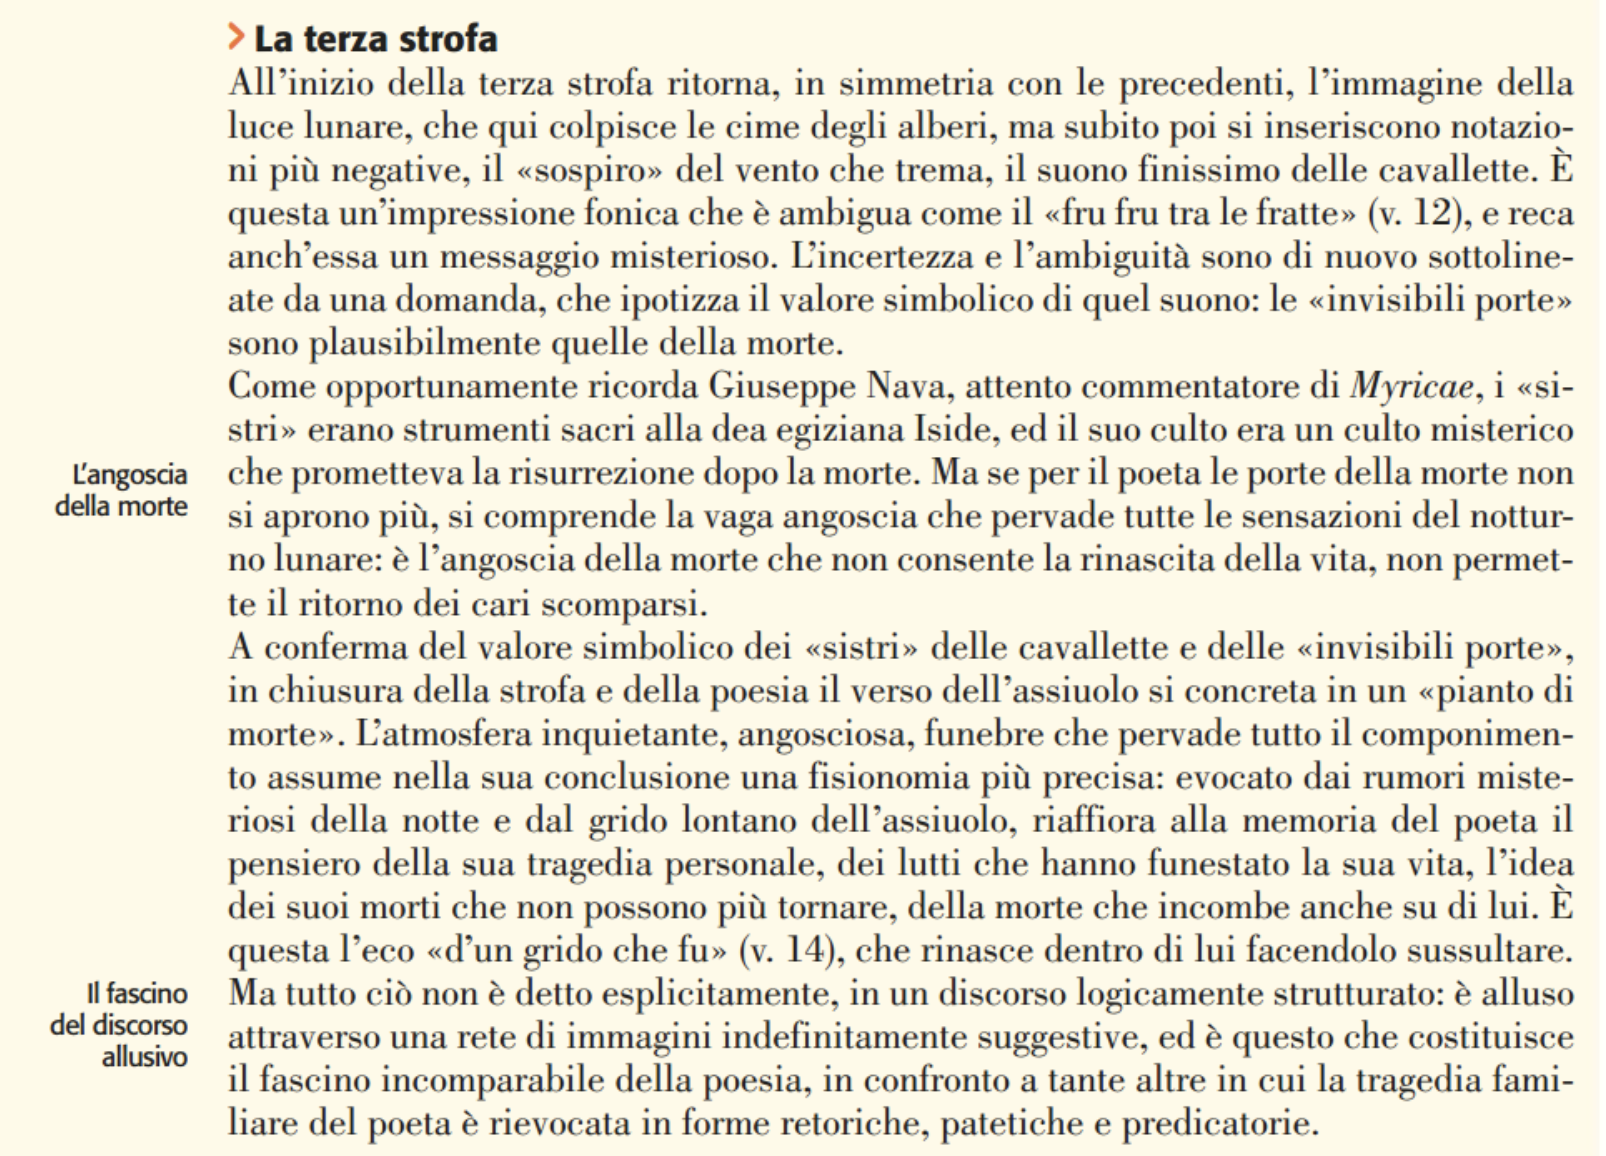
\includegraphics[width=\textwidth]{assiuolo4}
\end{center}

\begin{center}
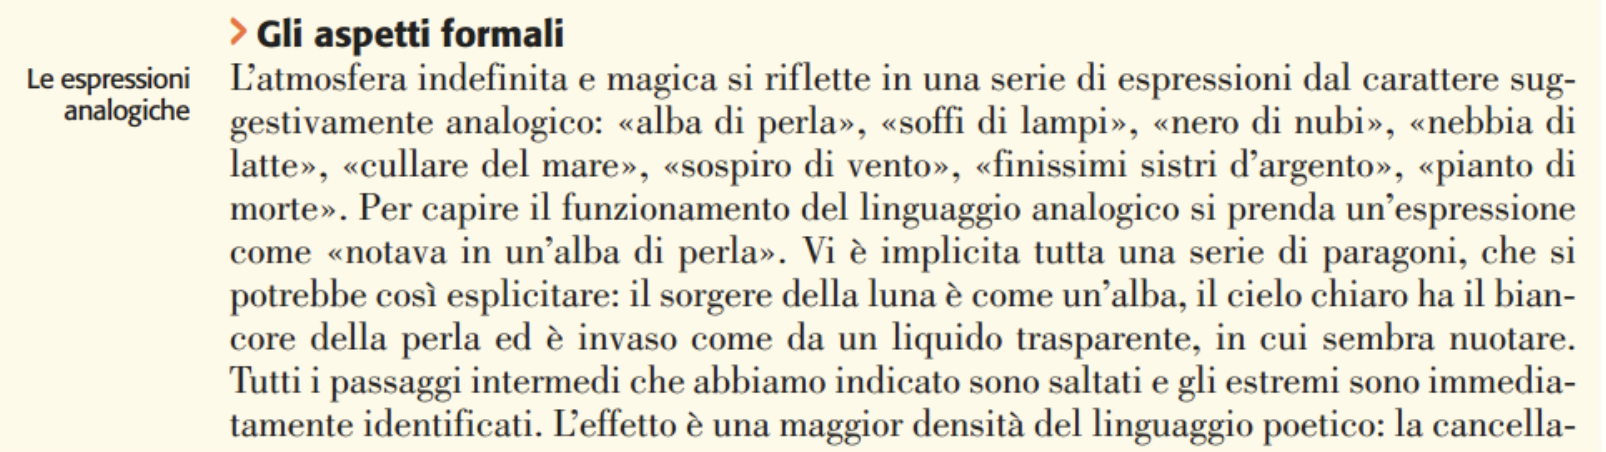
\includegraphics[width=\textwidth]{assiuolo5}
\end{center}
\vfill
\begin{center}
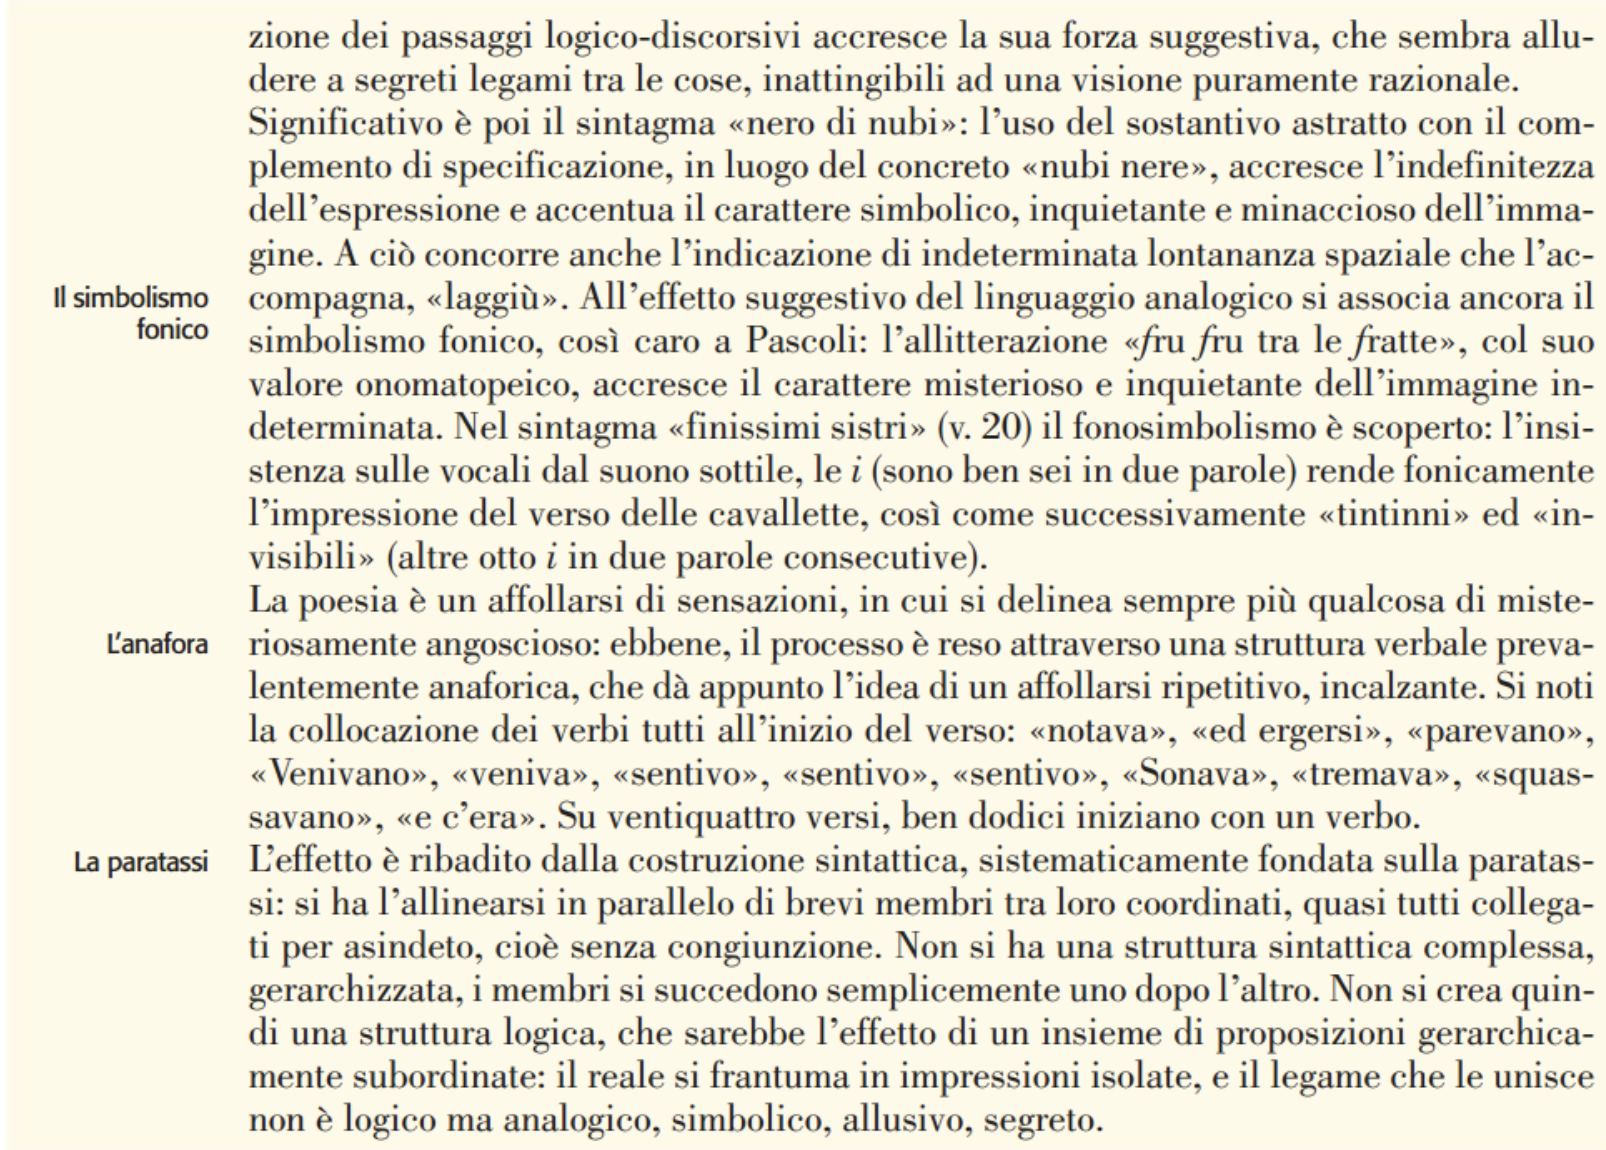
\includegraphics[width=\textwidth]{assiuolo6}
\end{center}

\section{T: \textit{Temporale}}

Non riusciamo a capire questa poesia se non guardando il titolo. Sono quasi ermetiche, fatte di suggestioni molto personali.

Il termine \textbf{impressionismo} viene utilizzato molto spesso nell'analizzare la poesia di Pascoli.

La poesia all'apparenza potrebbe sembrare un bozzetto impressionistico, con note di colore qua e là, ma in realtà non è così.
In letteratura l'esperienza del temporale ha sembra avuto valenza simbolica: da Boccaccio, per cui rappresenta un'insidia per la vita dell'uomo.
In Pascoli la tempesta ha un significato ancora più profondo: c'è un aspetto della sua biografica che è una sorta di punto fermo nella sua vita, un grande dolore che Pascoli ha vissuto da bambino: il temporale suscita paura.
Quello che ci vuole esprimere Pascoli non è tanto la funzione simbolica, lui ci vuole proprio far sentire la paura che si vive durante il temporale.

\setcounter{mar}{0}
\begin{verse}
Un bubbolìo lontano...\\!
Rosseggia l’orizzonte,\\
come affocato\mat{non si capisce se sia riferito a ``orizzonte'' o a ``mare''}, a mare:\\
nero di pece, a monte,\\
stracci di nubi chiare:\\
tra il nero un casolare:\\
un’ala di gabbiano\mat{per analogia è associato al casolare}.
\end{verse}

Si può notare la sintassi frantumata, sono tutti accostamenti, è difficile fare l'analisi del periodo: non c'è una sintassi compiuta. La sintassi frantumata allude a quella realtà che non ha più un ordine, che è frantumata per il soggetto, ma non solo: le esperienze personali del poeta diventano esperienze dell'umanità.

Guardando la poesia senza titolo potremmo anche non sapere quale sia il soggetto della poesia: questo aspetto sarà poi tipico della poesia ermetica, in cui il titolo diventa parte integrante del testo stesso, perché molto spesso noi non sapremmo neanche di cosa si stia parlando senza il titolo.

\elenco{\item \textbf{v.1}: \textit{bubbolio} è una onomatomea: è spesso usata in Pascoli; è una figura retorica che o riproduce il suono di qualcosa, oppure è un termine che riproduce nell'accostamento dei suoni il suono della cosa a cui si allude; \textit{bubbolio lontano} fa riferimento al rumore rombante di quando si avvicina il temporale
\item \textbf{v. 2}: \textit{rosseggia l'orizzonte}: note di colore; colori e suoni sono sempre molto presenti nelle poesie di Pascoli, perché sono queli elementi che trasmettono sensazioni: queste note di colore sono quelle che lo fanno definire "impressionista"
\item \textbf{v. 4}: \textit{nero di pece a monte}: molto spesso Pascoli utilizza queste espressioni: con questa scelta sembra di toccare più concretamente questo concetto: abbiamo spesso questo meccanismo: un sostantivo, il "di", e poi una cosa materiale
\item \textbf{v.5}: \textit{stracci di nubi chiare}: ecco un esempio di analogia; stracci fa allusione a qualcosa di stracciato, spezzato; stesso meccanismo di prima.
\item \textbf{v. 7}: il volo ha accezione positiva: associare la casa all'ala di gabbiano (conoscendo il valore della casa per Pascoli) gli da un valore consolatorio, quasi ottimistico.
}

\begin{center}
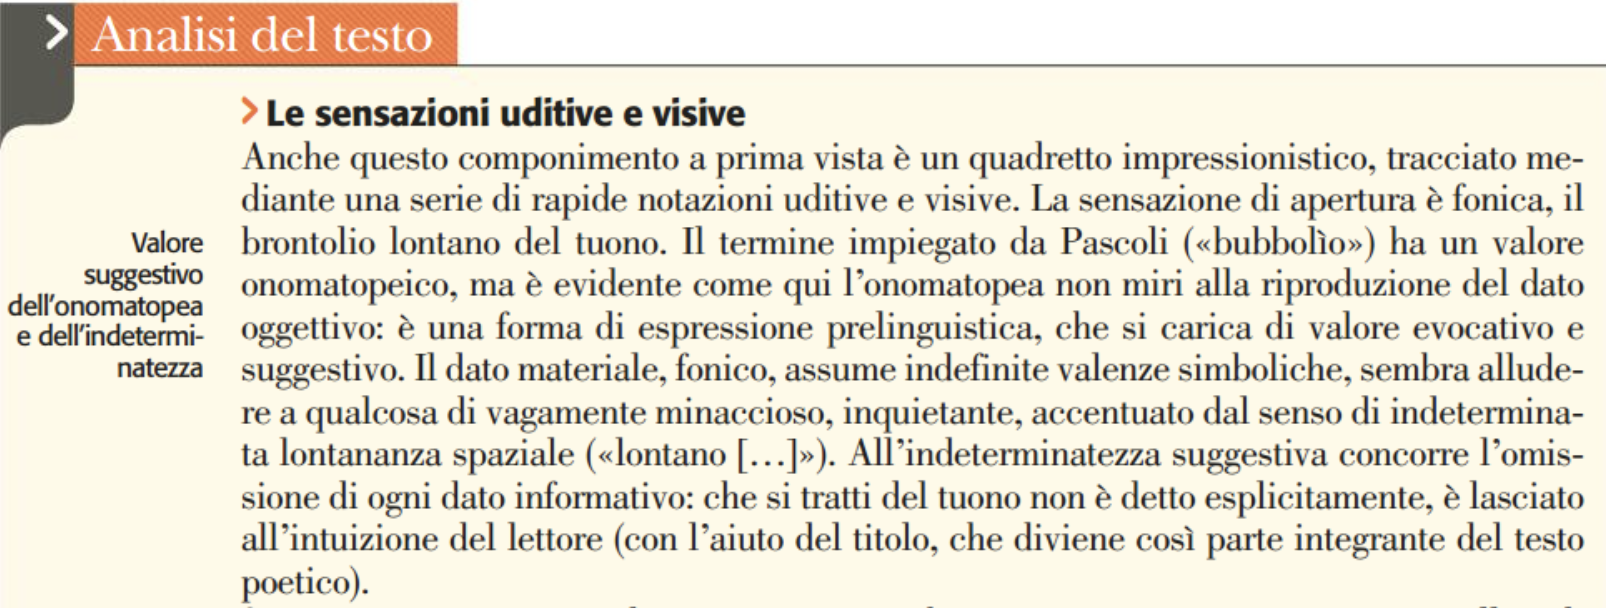
\includegraphics[width=\textwidth]{temporale1}
\end{center}

\begin{center}
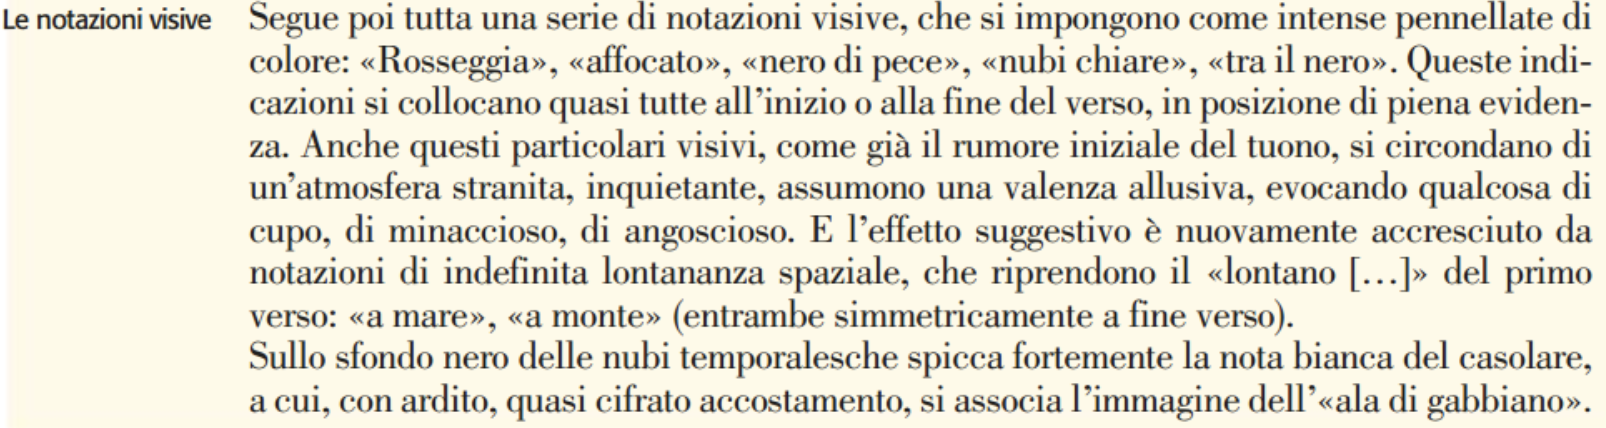
\includegraphics[width=\textwidth]{temporale2}
\end{center}
\vfill
\begin{center}
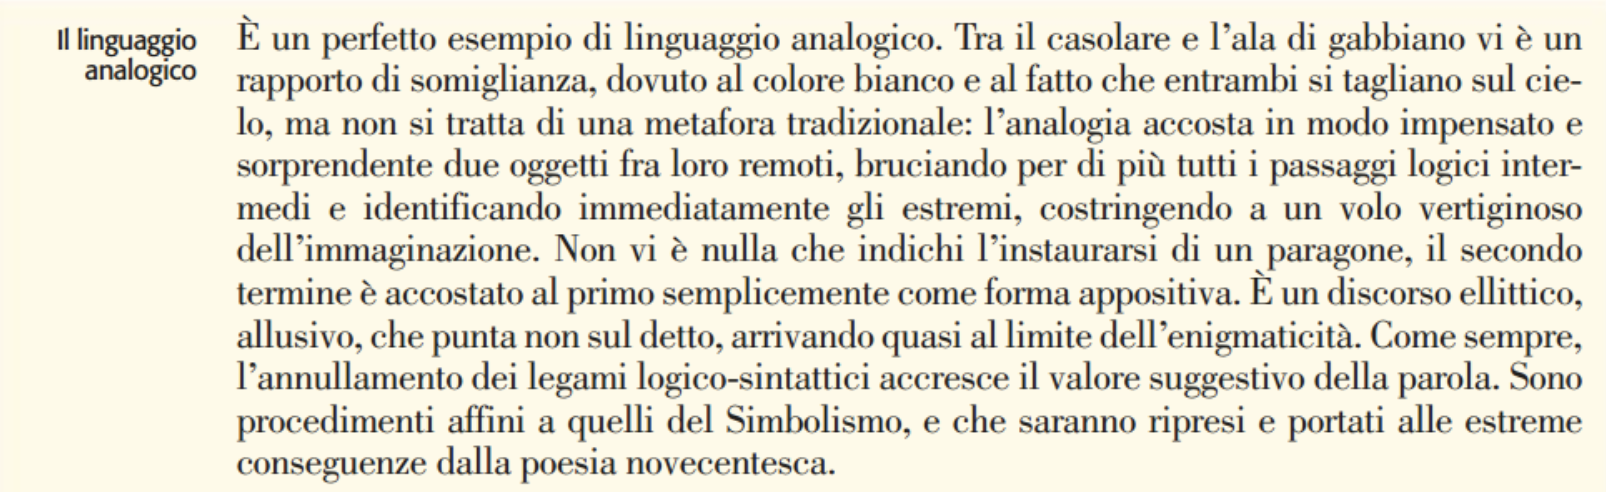
\includegraphics[width=\textwidth]{temporale3}
\end{center}

\begin{center}
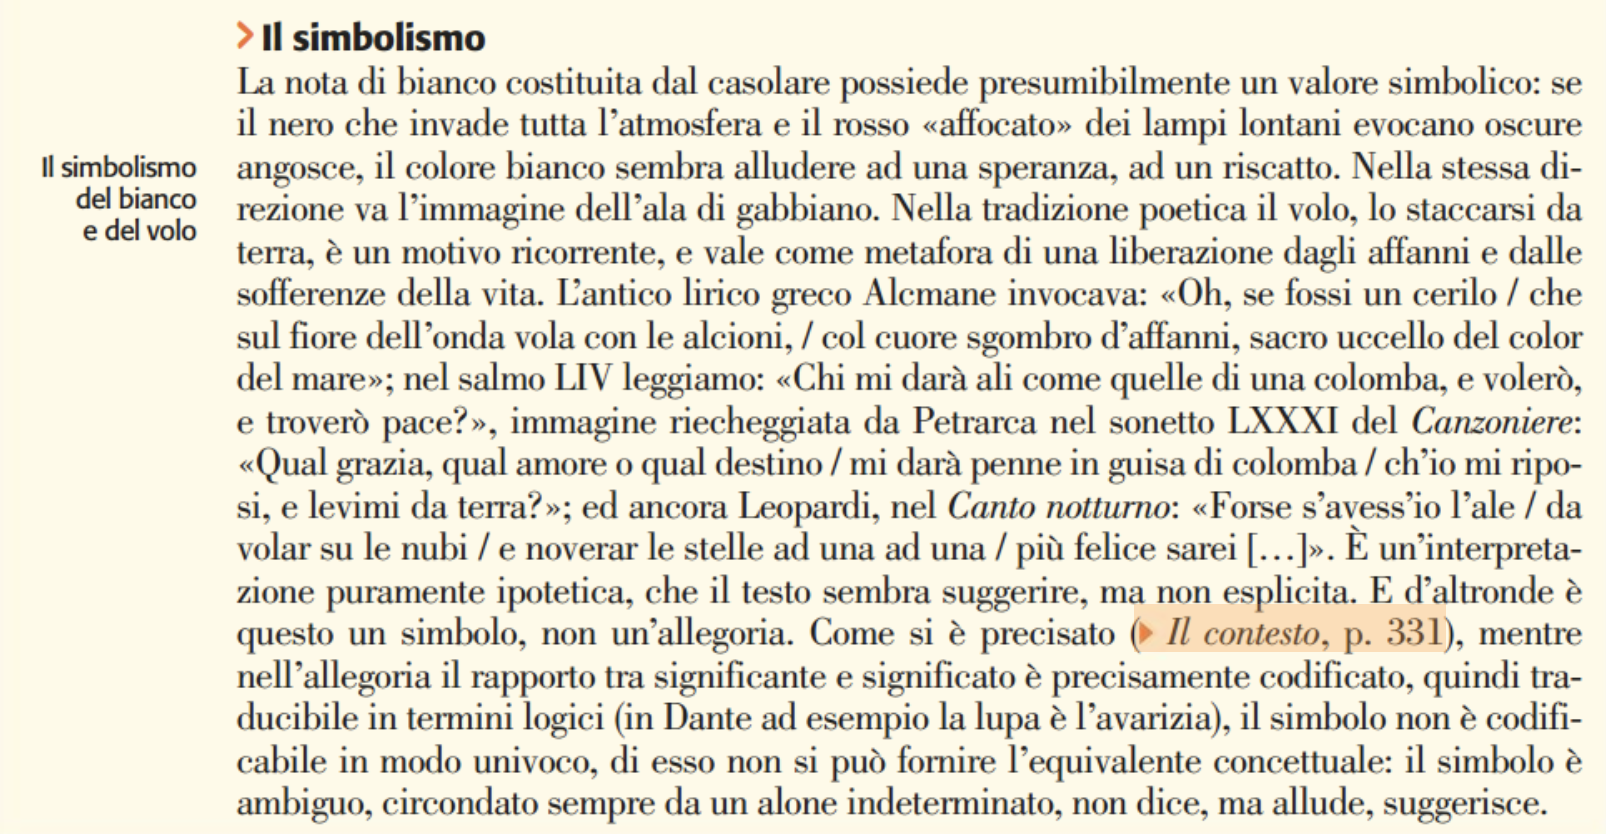
\includegraphics[width=\textwidth]{temporale4}
\end{center}

\section{T: \textit{Novembre}}

Questa lirica sarà molto apprezzata da Carducci.
Abbiamo una strofa saffica.
Pascoli usa una forma che si lega alla tradizione classica, a cui opera delle distorsioni e delle inarcature che rendono evidenti alcuni temi; sono scelte che stupiscono in questo tipo di struttura.

Nella prima strofa viene messa in moto l'illusione

\setcounter{mar}{0}
\begin{verse}
Gemmea\mat{aggettivo, ma molto forte} l’aria, il sole così chiaro\\
che tu ricerchi gli albicocchi in fiore,\\
e del prunalbo l’odorino amaro\mat{sinestesia}\\
\hspace{8em}senti nel cuore\mat{con l'immaginazione}...\\!
Ma secco è il pruno, e le stecchite piante\\
di nere trame segnano il sereno\mat{cielo},\\
e vuoto il cielo, e cavo al piè sonante\mat{riferito al passo}\\
\hspace{8em}sembra il terreno.\\!
Silenzio, intorno: solo, alle ventate,\\
odi lontano, da giardini ed orti,\\
di foglie un cader fragile\mat{ipallage e sinestesia, onomatopea con \texttt{f} e \texttt{r}}. È l’estate,\mat{enjambement molto forte}\\
\hspace{8em}fredda\mat{\textit{estate fredda}: ossimoro}, dei morti.\\!
\end{verse}

Solito bozzetto paesaggistico e impressionistico, che è simbolo di qualcosa. Novembre è simbolo di una stagione dell'anima.
In questa poesia abbiamo ben chiaro il sentimento di disillusione.

Novembre è uno dei mesi più bui e tristi: l'inverno sta iniziando ed è ancora molto lungo. Inoltre è la stagione dei morti.

Abbiamo una atmosfera ingannevole, in quanto l'atmosfera è gemmea, e ci sono segnali che ci fanno sembrare sia un giorno di primavera. Siamo disillusi al \textbf{verso 5}, con quel \textit{Ma secco}, quando il tema diventa quello dei morti.

È difficile dire di cosa parli la poesia: parla di sentimenti, sensazioni che durano qualche istante

Nell'ultima strofa vediamo molti segni di punteggiatura forti: Pascoli forza la grammatica per isolare e strappare determinati termini. La poesia è circolare per forte contrasto.

\begin{center}
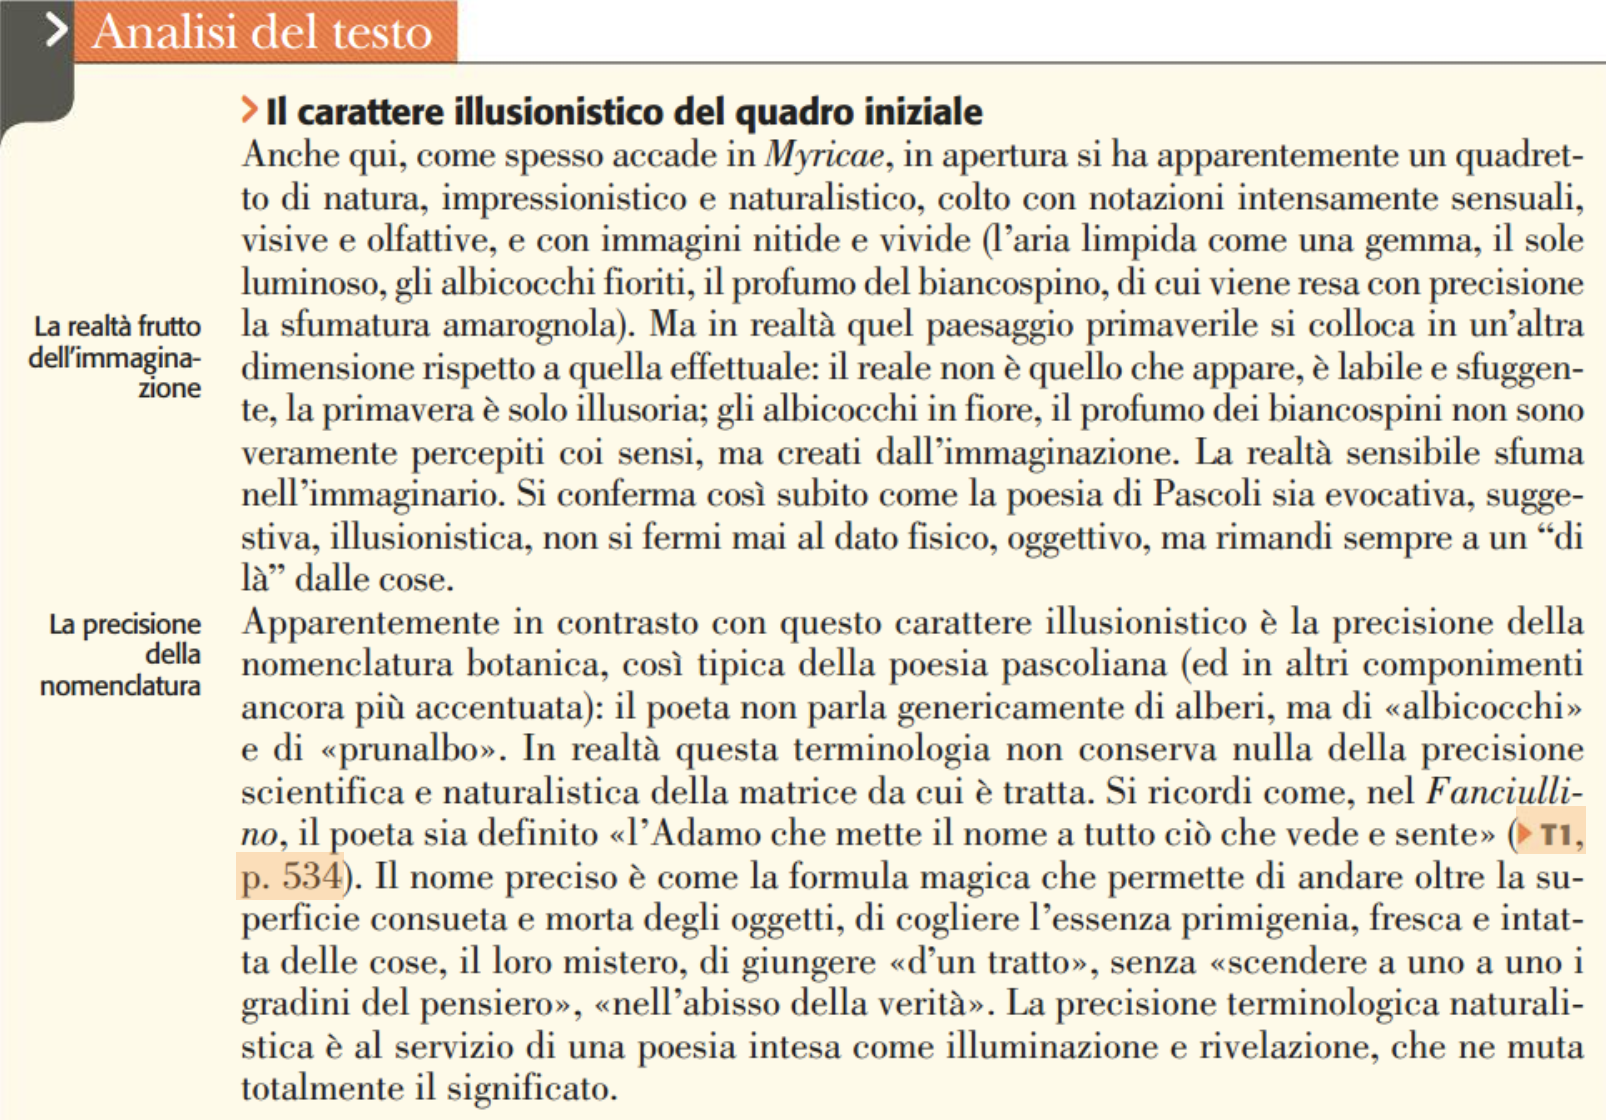
\includegraphics[width=\textwidth]{novembre1}
\end{center}
\vfill
\begin{center}
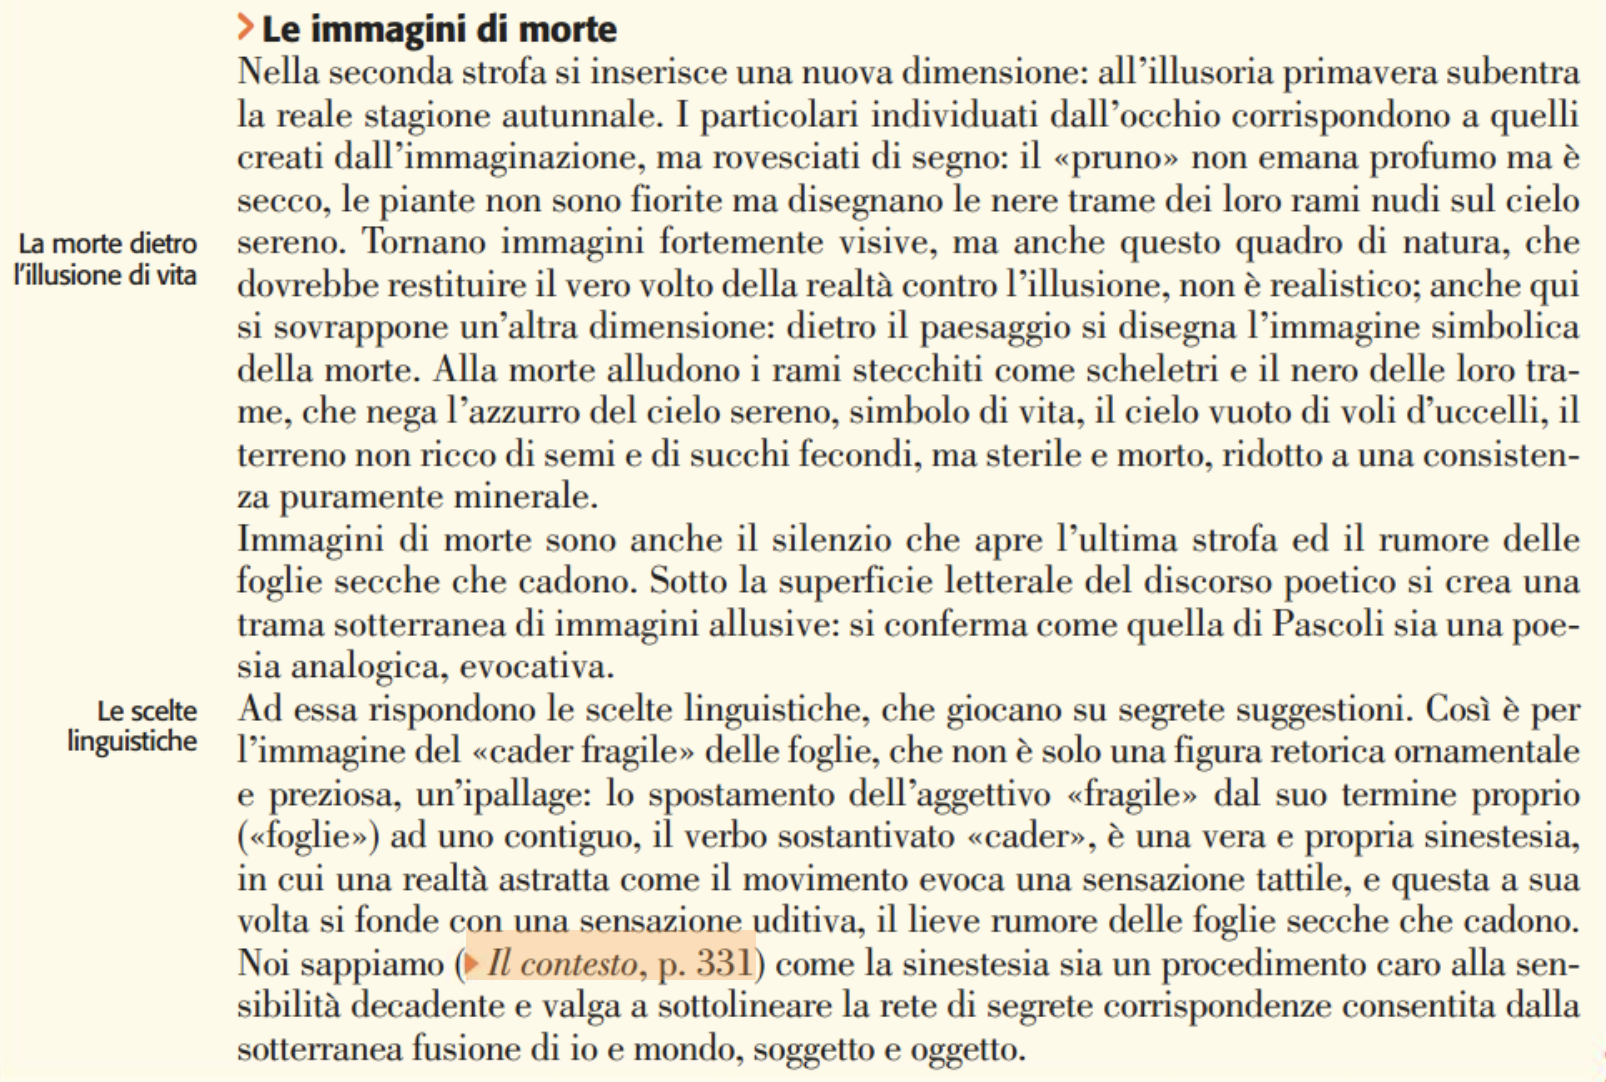
\includegraphics[width=\textwidth]{novembre2}
\end{center}

\begin{center}
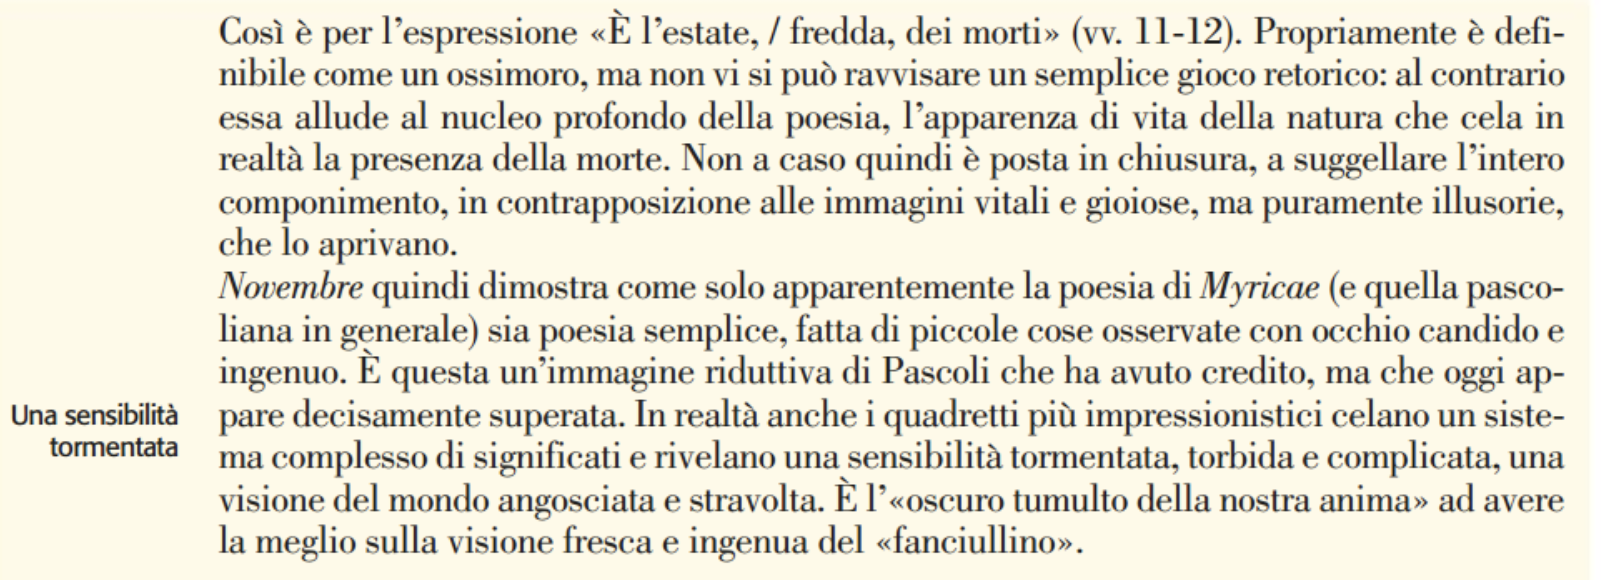
\includegraphics[width=\textwidth]{novembre3}
\end{center}

\begin{center}
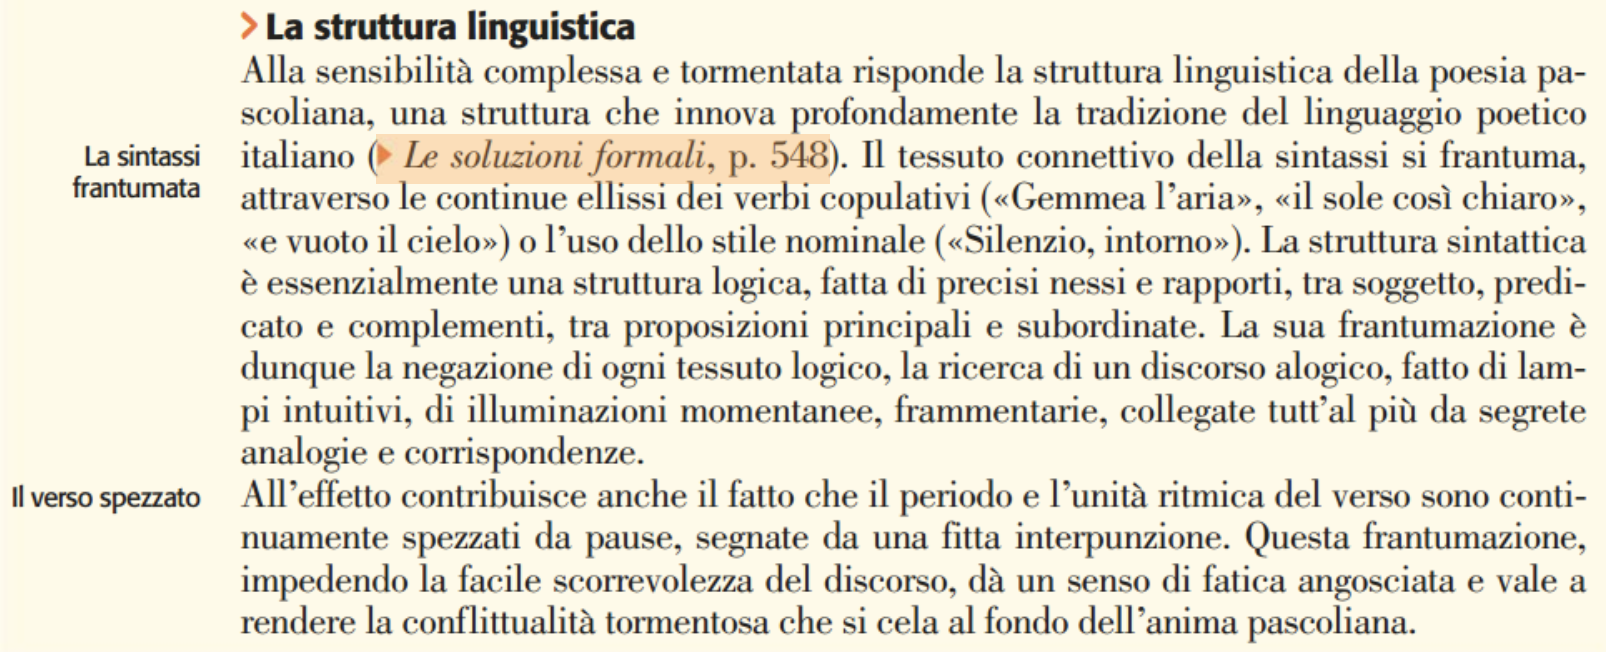
\includegraphics[width=\textwidth]{novembre4}
\end{center}

\section{T: \textit{Il lampo}}

Da una prefazione in edita la terza edizione di \textit{Myricae} apprendiamo che fu concepito come metafora degli ultimi momenti del padre morente: "i pensieri che tu, o padre mio benedetto, facesti in quel momento, in quel batter d'ala - Il momento fu rapido [...] ma i pensieri non furono brevi e pochi. Quale intensità di passione! Come un lampo in una notte buia: dura un attimo e ti rivela tutto un cielo pezzato, lastricato, squarciato, affannato, tragico". A questa tematica si lega l'immagine finale dell'occhio aperto e subito richiuso, che richiama l'ultimo sguardo di un moribondo.

Fa parte della trilogia: \textit{Il temporale}, \textit{Il lampo} e \textit{Il tuono}

\setcounter{mar}{0}
\begin{verse}
E cielo e terra\mat{polisindedo: senso di affanno} si mostrò qual era:\mat{nel momento in cui c'è il fulmine}\\!
la terra ansante, livida, in sussulto;\\
il cielo ingombro, tragico, disfatto:\\
bianca bianca\mat{simile all'``ala di gabbiano'' del Temporale, riferito ad ``una casa'', nel verso successivo} nel tacito tumulto\mat{espressione ossimorica}\\
una casa apparì sparì\mat{asindedo} d’un tratto;\\
come un occhio, che, largo, esterrefatto,\\
s’aprì si chiuse, nella notte nera.
\end{verse}

Ci trasmette una sensazione di paura, e nello spavento generale una visione: il lampo per un istante illumina a giorno la scena; la luce anziché confortare crea uno sgomento ancora maggiore, ed è lo stesso sgomento che avrebbe provato il padre sbarrando gli occhi prima di morire.

In questa poesia non si può più parlare di impressionismo di Pascoli, ma quasi di espressivismo: il poeta vuole esasperare determinati aspetti.

A differenza di altri componimenti di \textit{Myricae}, qui le impressioni visive non hanno neppure l'apparenza di oggettività impressionistica, sono immediatamente connotate da un valore simbolico e dotate di una forte carica espressionistica, portate ad un estremo di tensione deformante: si noti la terra che all'improvviso chiarore del lampo appare "ansante, livida, in sussulto" (\textbf{v. 2}), il cielo "ingombro, tragico, disfatto" (\textbf{v. 3}), la bianca casa paragonata all'occhio che si apre "largo, esterrefatto" per chiudersi subito dopo.


\chapter{I \textit{Poemetti}}

\elenco{\item \emph{p. 573}}

I \textit{Poemetti} vengono composti in diverse tappe, dal 1897 al 1909: con l'ultima edizione se ne aggiungono sempre di più rispetto alle precedenti.
Il tempo di composizione corrisponde a quello di \textit{Myricae}.
Le due opere sono profondamente diverse: i poemetti hanno una struttura prevalentemente narrativa, quindi anche se sono in versi sono composizioni molto più lunghe rispetto a quelle di \textit{Myricae}

Questa serie di poemetti va quasi a formulare un racconto; molti di essi sono collegati a due personaggi, Rigo e Rosa, collocati nel contesto campestre.
Infatti molti hanno riscontrato una forte analogia con le \textit{Georgiche} di Virgilio: l'ambientazione è la campagna, e nei vari poemetti sono descritti tutti i ritmi della natura e del lavoro in campagna. Oltre a questa lezione di Virgilio, è presente anche la lezione di Esiodo, con la sua opera \textit{Le opere e i giorni}.

L'opera viene intesa da molti come una sorta utopia regressiva, in quanto Pascoli riflette il suo ideale di vita della campagna (positivo, perché rappresenta una sorta di protezione nei confronti del mondo attuale, della politica e della violenza), però proiettato nel passato e non nel futuro. Pascoli non sembra cogliere tutti quegli aspetti negativi che erano invece presente in Verga.

\section{Posizioni politiche}

Non coglie la lotte di classe caratteristica di Verga: il suo atteggiamento è quello di una sorta di filantropia umanitaria, di tipo cristiano, che consiste in una sorta di benevolenza ed empatia nei confronti degli altri uomini; questo resta del suo socialismo.

Negli ultimi anni della sua vita Pascoli addirittura abbraccia posizioni nazionalistiche, e di favore nei confronti delle guerre per la fondazione di nuove colonie: nel 1911 appoggia con entusiasmo la guerra di Libia. In realtà c'è una spiegazione logica a questo atteggiamento, che si cala in un periodo estremamente negativo per il poeta: l'ultima parte della sua vita è rattristata e angustiata dalla malattia e da una serie di timori che serpeggiavano in europa e in Italia e che sfocieranno nella Prima Guerra Mondiale.

La sua approvazione nei confronti della guerra di Libia aveva all'origine una sorta di sentimento di Pietà, di empatia, di preoccupazione per tutti gli emigranti italiani come ad esempio Italy. Questa odissea dei migranti era vissuta con preoccupazione e tristezza che lo porta a vedere nella guerra Per le coloni una sorta di ricompensa è una sorta di soluzione. E come se questi migranti che sono stati sradicati dal nido avrebbero potuto ritrovare sostanzialmente una patria, un compenso, anche se a spese di altre popolazioni.

\section{T: \textit{Digitale purpurea}}

Come filo portante di tutti i puoi metti ce la vita di campagna, i lavori dei campi. La vicenda non è ricostruita, si può immaginare che ci sia qualcosa dietro questo scambio di battute tra due donne.
\textbf{Digitale purpurea} era il nome di un fiore: ricordiamo che i fiori avevano un grande fascino nella letteratura decadente, ed in particolare alcuni fiori simbolici; la digitale purpurea ha dei petali che possono sembrare delle dita, di un rosso molto intenso, abbinato alla passione amorosa. Pascoli quando parla dell'amore ne parla sempre attraverso immagini simboliche, quasi sempre tratte dal mondo della natura.

Sono rappresentate due donne che si incontrano e parlano di un avvenimento che risale ai tempi del collegio. La sorella di Pascoli, Maria, si è pronunciata a distanza di anni su questo poemetto: una delle due donne del poemetto si chiama proprio Maria, e rappresenta lei stessa, mentre non sa a chi alludesse il fratello con la figura delle altra donna, rachele.
Molti pensano che rachele rappresenti simbolicamente Ida, l'altra sorella di Pascoli, che si è sposata.
Rachele rappresenta sostanzialmente l'attrazione per l'eros, e quindi potrebbe fare riferimento a Ida, che a differenza di Pascoli e della sorella Maria avrebbe affrontato il grande passo di cercare di ricostruire un nuovo nido.

Il poemetto si apre con una sorta di flashback, un ricordo della loro fanciullezza.

\subsection*{I}

\begin{verse}
\poemlines{3}
Siedono. L’una guarda l’altra. L’una\\
esile e bionda, semplice di vesti\\
e di sguardi; ma l’altra, esile e bruna,\\!
l’altra... I due occhi semplici e modesti,\\
fissano gli altri due ch’ardono. “E mai,\\
non ci tornasti?„ “Mai„ “Non le vedesti\\!
più?„ “Non più, cara„ “Io si: ci ritornai;\\
e le rividi le mie bianche suore,\\
e li rivissi i dolci anni che sai;\\!
quei piccoli anni così dolci al cuore...„\\
L’altra sorrise “E di’: non lo ricordi\\
quell’orto chiuso? i rovi con le more?\\!
i ginepri tra cui zirlano i tordi?\\
i bussi amari? quel segreto canto\\
misterïoso, con quel fiore, fior di...?„\\!
“morte: sì, cara„ “Ed era vero? Tanto\\
io ci credeva che non mai, Rachele,\\
sarei passata al triste fiore accanto.\\!
Chè si diceva: il fiore ha come un miele\\
che inebria l’aria; un suo vapor che bagna\\
l’anima d’un oblìo dolce e crudele.\\!
Oh! quel convento in mezzo alla montagna\\
cerulea!„ Maria parla: una mano\\
posa su quella della sua compagna;\\!
e l’una e l’altra guardano lontano.
\end{verse}

\elenco{\item \textbf{verso 1-5}: ecco i due tipi di donna, la donna angelica e la \textit{femmé fatale}; per farci capire quanto queste due donne siano diverse, "\textit{l'altra...}" è spostata nel verso successivo; gli occhi ardenti della femme fatale alla fine di questa poesia vengono ripresi
\item \textbf{verso 10}: \textit{piccoli anni}: sono piccole loro, non gli anni
\item \textbf{versi 12-14}: la precisione con cui vengono nominate le piante è tipica di Pascoli; \textit{zirlano}: è il verso del tordo;
\item \textbf{verso 14}: \textit{quel segreto canto}: sta per cantuccio
\item \textbf{verso 15}: \textit{fior di...?}: enjambement, sostenuto dai punti di sospensione e dal punto interrogativo
\item \textbf{verso 15-16}: \textit{fior di morte}: fa riferimento proprio alla digitale purpurea: questo fiore rappresenta un divieto (le bambine del collegio avevano il divieto di avvicinarsi a questo fiore)
}
La poesia è piena di gesti, di immagini, sguardi, piuttosto inquietanti

\elenco{\item \textbf{versi 16-18}: Maria ha veramente paura di quello che si dice del fiore
}

\subsection*{II}

\begin{verse}
Vedono. Sorge nell’azzurro intenso\\
del ciel di maggio il loro monastero,\\
pieno di litanie, pieno d’incenso.\\!
Vedono; e si profuma il lor pensiero\\
d’odor di rose e di viole a ciocche,\\
di sentor d’innocenza e di mistero.\\!
E negli orecchi ronzano, alle bocche\\
salgono melodie, dimenticate,\\
là, da tastiere appena appena tocche...\\!
Oh! quale vi sorrise oggi, alle grate,\\
ospite caro? onde più rosse e liete\\
tornaste alle sonanti camerate\\!
oggi: ed oggi, più alto. Ave, ripete,\\
Ave Maria, la vostra voce in coro;\\
e poi d’un tratto (perchè mai?) piangete...\\!
Piangono, un poco, nel tramonto d’oro,\\
senza perchè. Quante fanciulle sono\\
nell’orto, bianco qua e là di loro!\\!
Bianco e ciarliero. Ad or ad or, col suono\\
di vele al vento, vengono. Rimane\\
qualcuna, e legge in un suo libro buono.\\!
In disparte da loro agili e sane,\\
una spiga di fiori, anzi di dita\\
spruzzolate di sangue, dita umane,\\!
l’alito ignoto spande di sua vita.
\end{verse}

Inizia l'immagine del passato.

Abbiamo una serie di espressioni, ricordi, immagini che si affollano nella mente delle due donne: sono ricordi estremamente lontani, e quindi riappaiono nella mente delle donne sottoforma di flash.

\elenco{\item \textbf{verso 4}: \textit{si profuma il lor pensiero}: la suggestione olfattiva va a sovrapporsi a quella visiva
\item \textbf{versi 10-11}: \textit{Oh! quale vi sorrise oggi, alle grate, ospite caro?}: questo verso ha dato origine a due interpretazioni:
  \elenco{\item alle grate le bambine magari possono ricevere degli ospiti
  \item potrebbe far riferimento a Cristo}
  Secondo Gioanola, l'ospite caro è Cristo, ricevuto nella comunione, che sorride della balaustra alle collegiali, le quali tornano al loro camerata in letizia infervorate dal sacramento ricevuto; secondo Baldi invece si tratta di qualche parente visto in parlatorio, magari un cuginetto, per cui le educande provano una segreta e inconsapevole attrazione; per questo tornano tutte eccitate nelle loro camerate. L'eros si traduce poi in un'intensificazione del misticismo (l'intonazione più alta con cui recita non l'ave maria), e l'eccitazione si trasforma in un pianto improvviso e immotivato.Pascoli rende qui in modo sottilmente allusivo i segreti i turbamenti della sensibilità adolescenziale. In particolare si inserisce nel clima impalpabilm
\item \textbf{verso 18}: il bianco è quello della divisa, ma è simbolo di purezza
\item \textbf{verso 22}: \textit{In disparte}: nel cantuccio di cui si faceva riferimento all'inizio.}

L'immagine simbolica dell'amore, il fiore, è accomunato dall'immagine della morte.

\subsection*{III}

\begin{verse}
“Maria!„ “Rachele!„ Un poco più le mani\\
si premono. In quell’ora hanno veduto\\
la fanciullezza, i cari anni lontani.\\!
Memorie (l’una sa dell’altra al muto\\
premere) dolci, come è tristo e pio\\
il lontanar d’un ultimo saluto!\\!
“Maria!„ “Rachele!„ Questa piange, “Addio!„\\
dice tra sè, poi volta la parola\\
grave a Maria, ma i neri occhi no: “Io,„\\!
mormora, “sì: sentii quel fiore. Sola\\
ero con le cetonie verdi. Il vento\\
portava odor di rose e di viole a\\!
ciocche. Nel cuore, il languido fermento\\
d’un sogno che notturno arse e che s’era\\
all’alba, nell’ignara anima, spento.\\!
Maria, ricordo quella greve sera.\\
L’aria soffiava luce di baleni\\
silenzïosi. M’inoltrai leggiera,\\!
cauta, su per i molli terrapieni\\
erbosi. I piedi mi tenea la folta\\
erba. Sorridi? E dirmi sentia, Vieni!\\!
Vieni! E fu molta la dolcezza! molta!\\
tanta, che, vedi... (l’altra lo stupore\\
alza degli occhi, e vede ora, ed ascolta\\!
con un suo lungo brivido...) si muore!„
\end{verse}

Si ritorna al presente: ci sono gesti un po' inquietanti: lo stringersi le mani le fa capire vicendevolmente, segno di un linguaggio loro, misterioso.

\elenco{\item \textbf{verso 5}: \textit{triste e pio}: citazione Dantesca, canto di Paolo e Francesca}

Ciò che Rachele ha comunicato con quella stretta di mano è che lei è venuta meno al divieto. Rachele non guarda negli occhi Maria.
Non spiega cosa è avvenuto, ma spiega lo stato d'animo in cui si trovava: la fanciulla sentiva ancora dentro di sé l'agitazione di un sogno fatto la notte; è tutto molto vago e indefinito, l'amore è vissuto da Pascoli come una sorta di tabù, come qualcosa di morboso e proibito.

\elenco{\item \textbf{versi 23-25}: vengono ripresi gli occhi ardenti descritti all'inizio; sono indizio della malattia che consuma Rachele: è allusivamente indicata com econseguenza della trasgressione}

\begin{center}
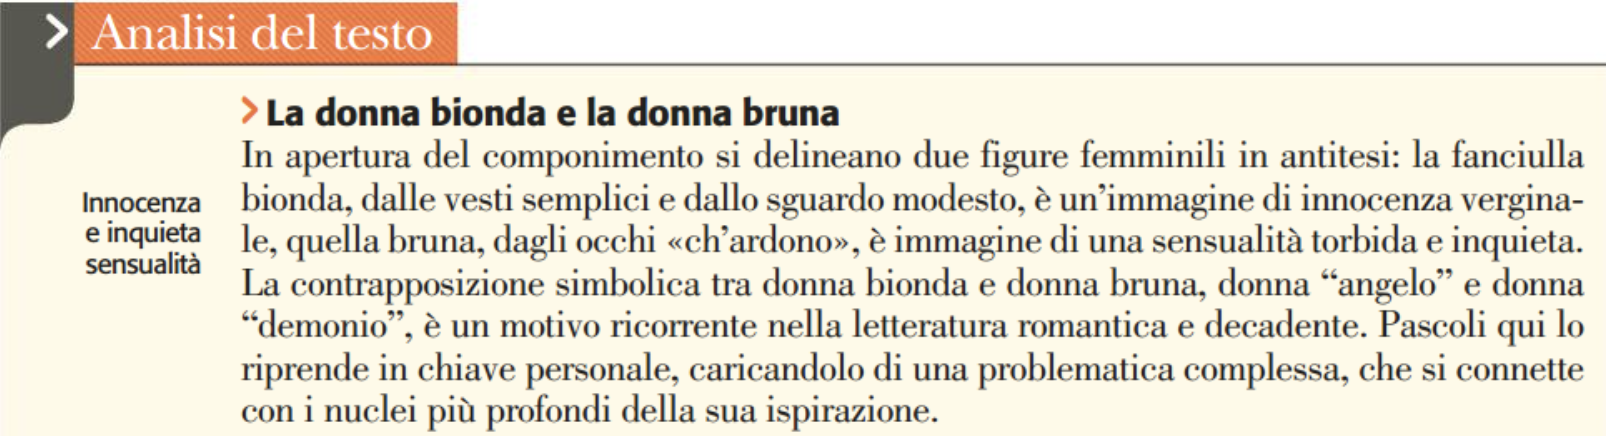
\includegraphics[width=\textwidth]{digitale1}
\end{center}

\begin{center}
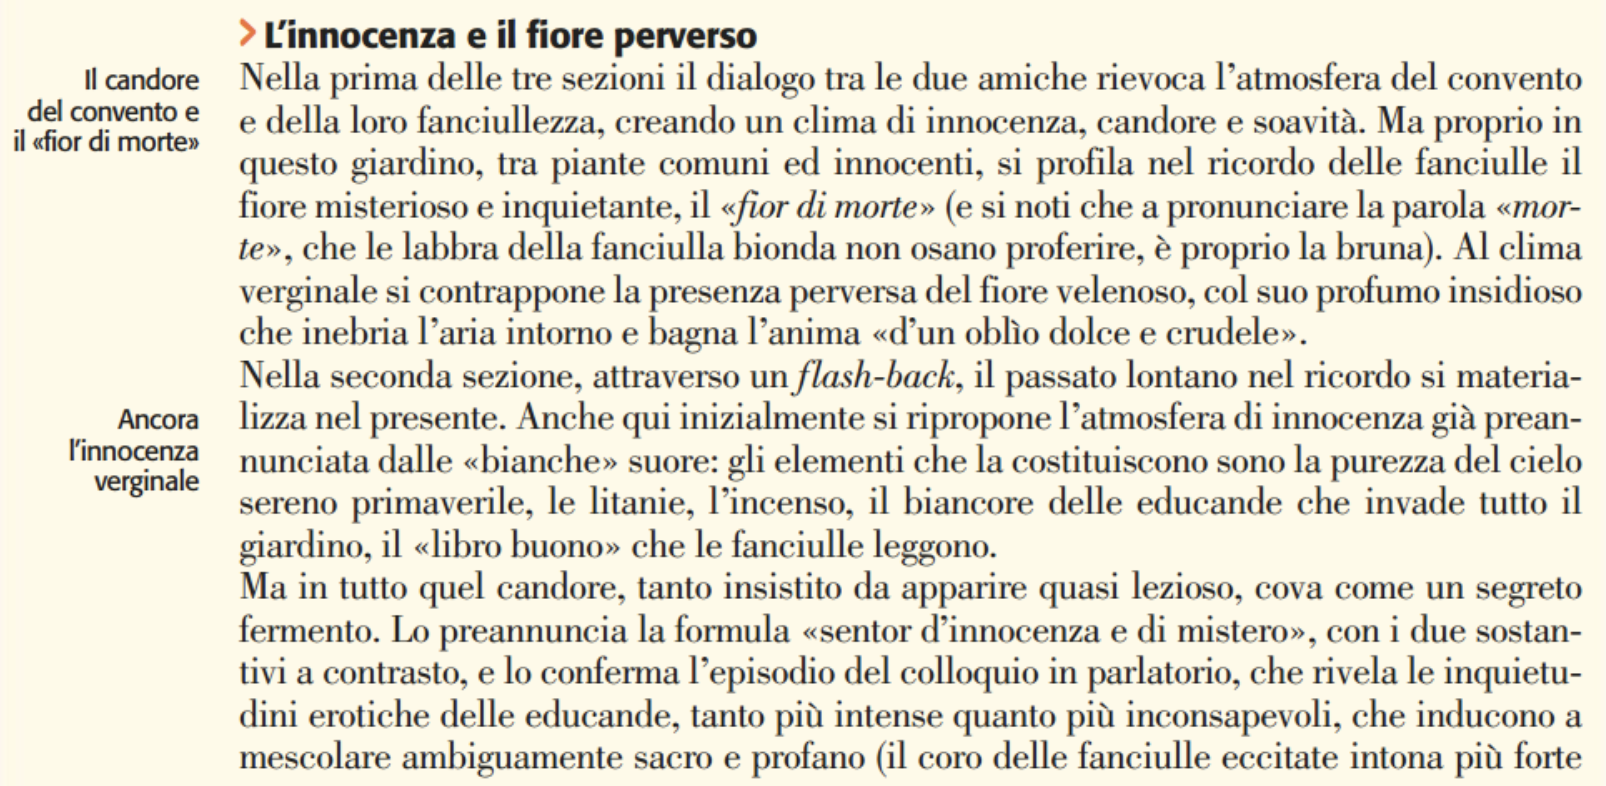
\includegraphics[width=\textwidth]{digitale2}
\end{center}

\begin{center}
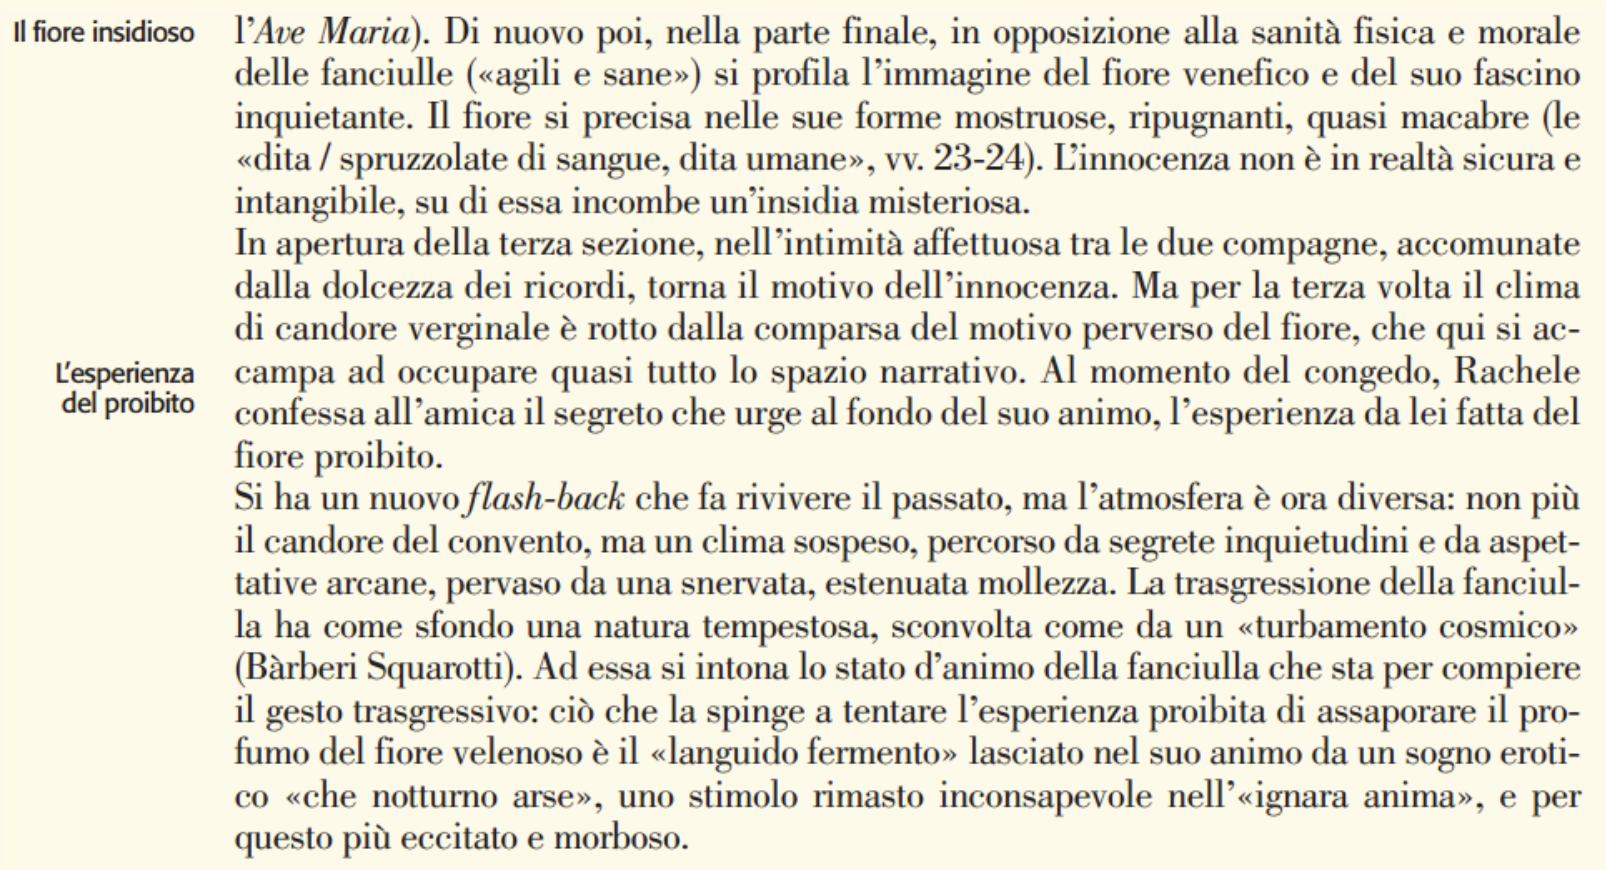
\includegraphics[width=\textwidth]{digitale3}
\end{center}
\vfill
\begin{center}
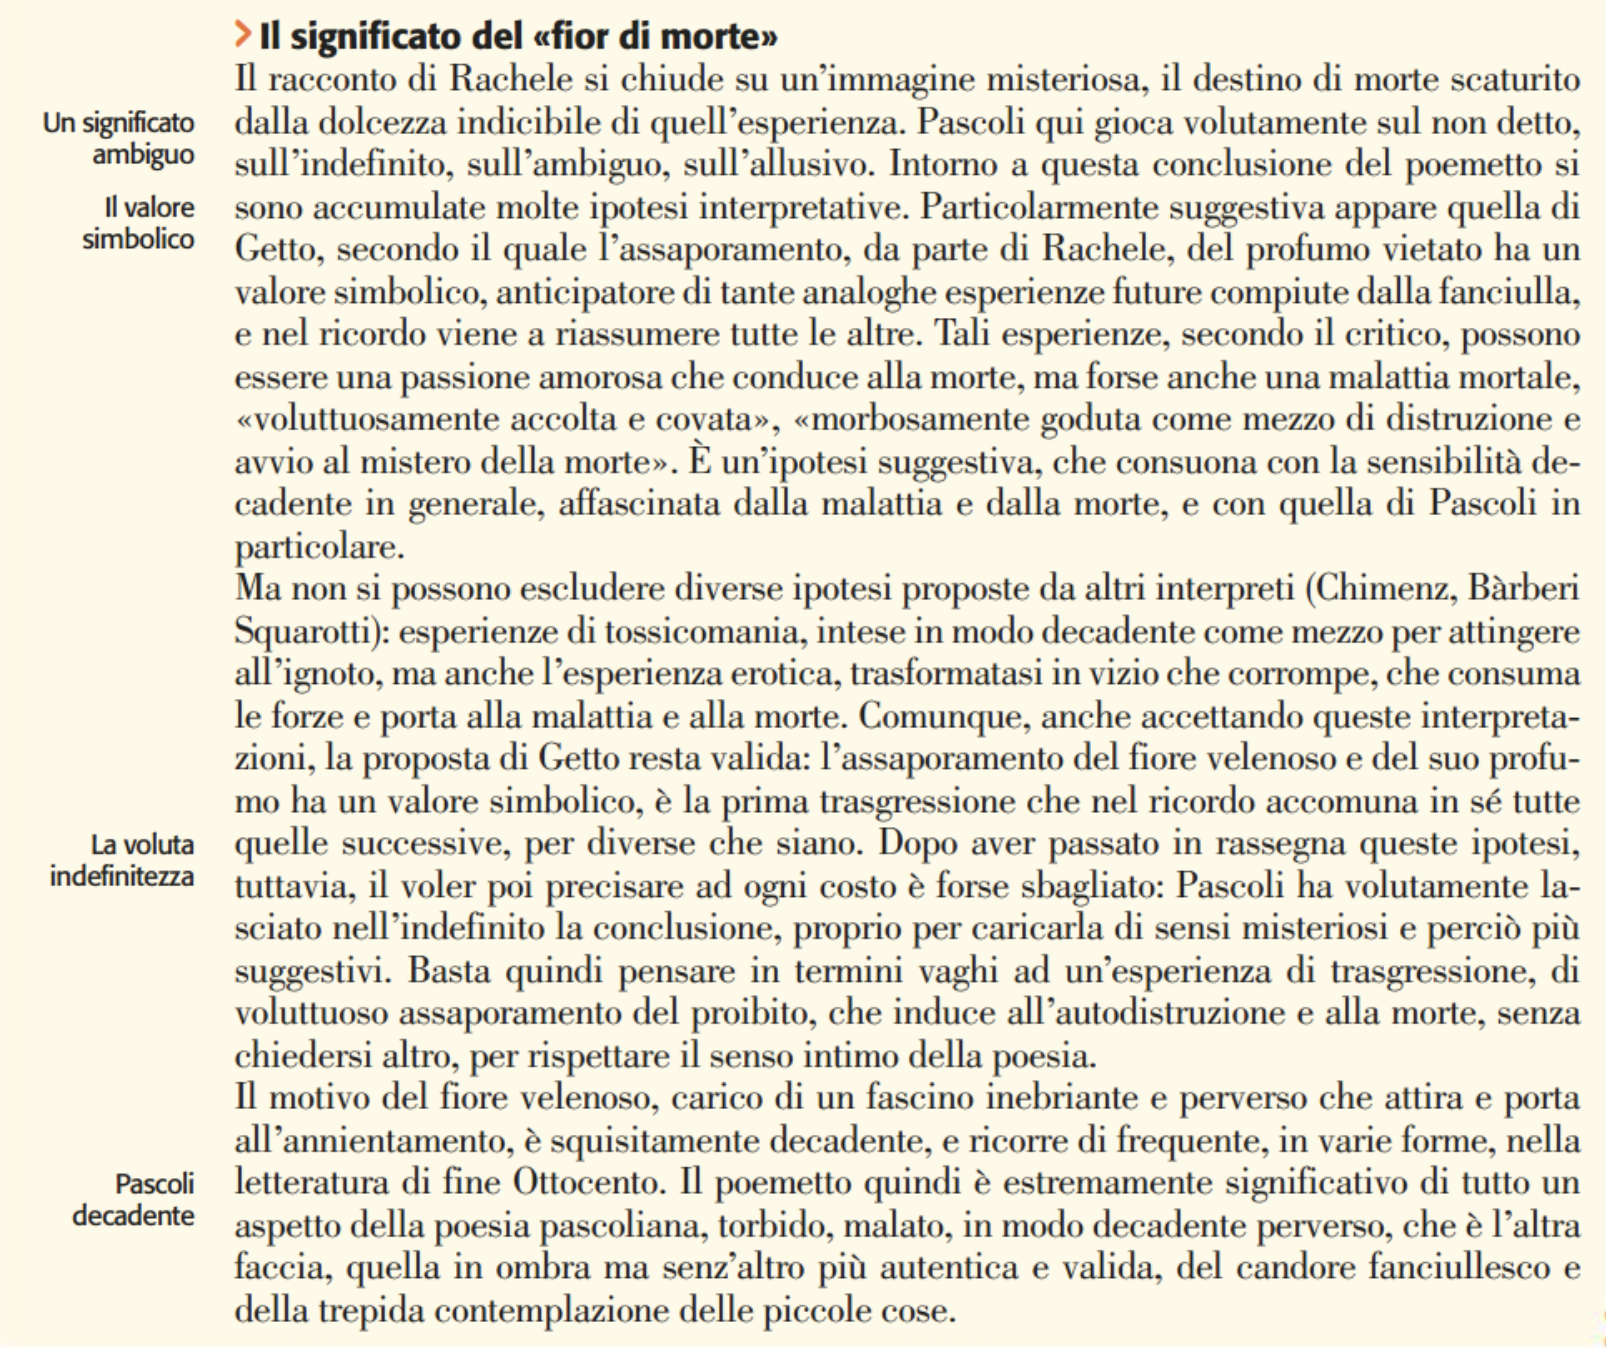
\includegraphics[width=\textwidth]{digitale4}
\end{center}

\begin{center}
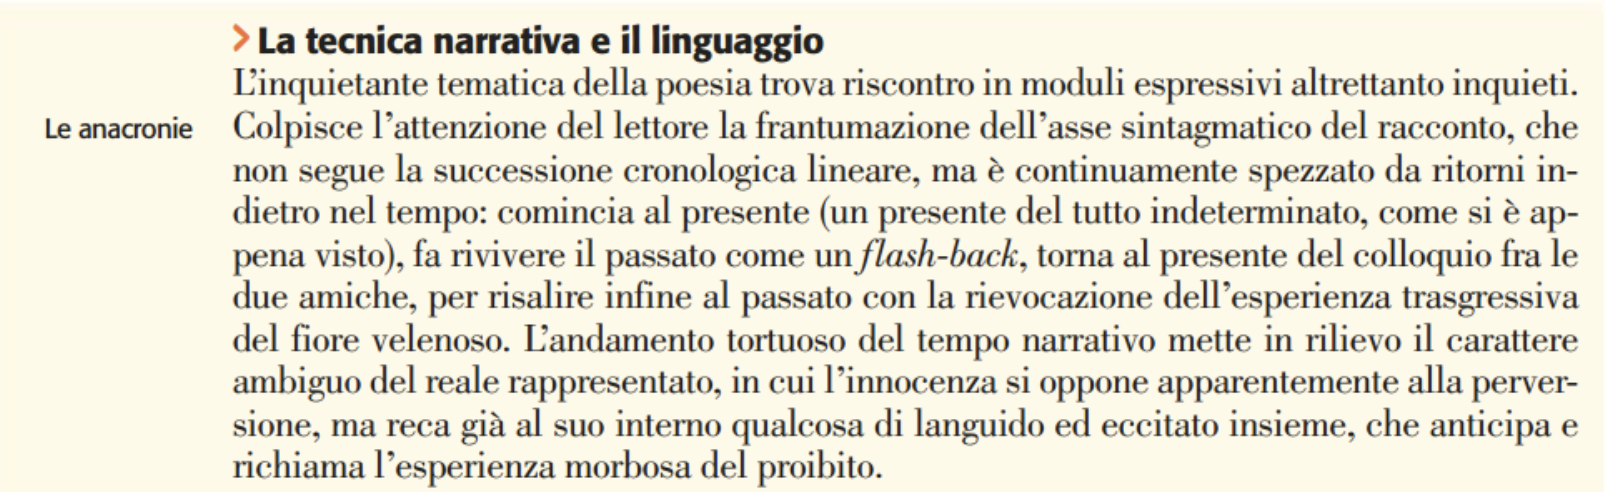
\includegraphics[width=\textwidth]{digitale5}
\end{center}

\begin{center}
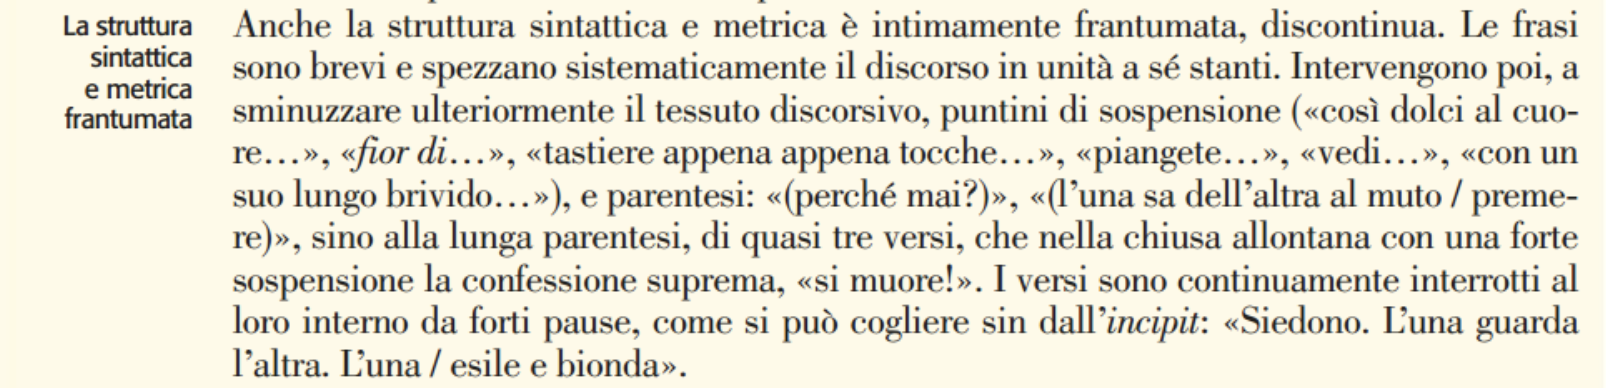
\includegraphics[width=\textwidth]{digitale6}
\end{center}
\vfill
\begin{center}
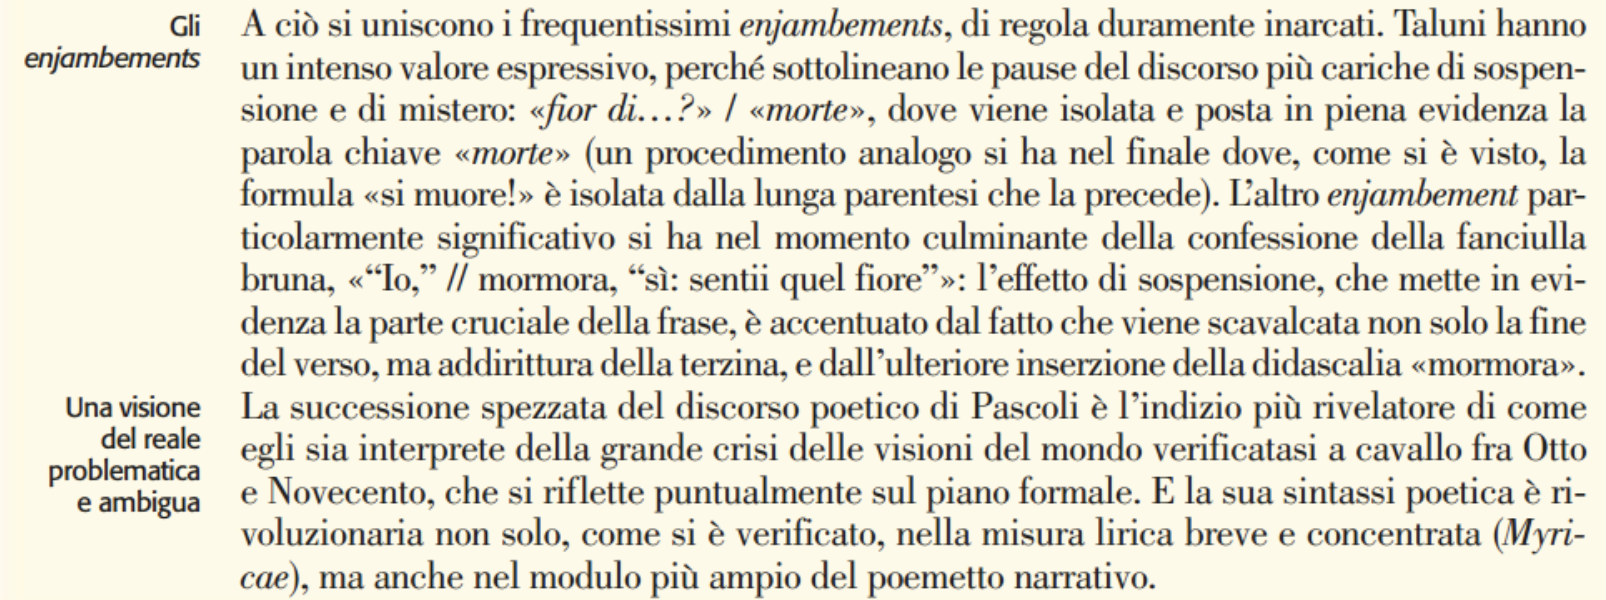
\includegraphics[width=\textwidth]{digitale7}
\end{center}

\chapter{T: \textit{Il gelsomino notturno}}

Fa parte della raccolta dei canti di Castelvecchio.
È un epitalamio, tipo di poesia scritta per le nozze.

\setcounter{mar}{0}
\begin{verse}
E\mat{allude ad una fase pre-festuale} s’aprono i fiori notturni,\\
nell’ora che penso ai miei cari.\mat{l'io lirico associa all'immagine serena il ricordo dei morti}\\
\vin Sono apparse in mezzo ai viburni\mat{termini botanici}\\
\vin le farfalle crepuscolari.\\!
Da un pezzo si tacquero i gridi\mat{sia i versi degli uccelli che le urla degli invitati}:\\
là sola una casa bisbiglia.\mat{ci mostra l'esclusione di Pascoli da questa gioia}\\
\vin Sotto l’ali dormono i nidi\mat{sostituzione con termini della natura},\\
\vin come gli occhi sotto le ciglia.\\!
Dai calici aperti si esala\\
l’odore di fragole rosse\mat{colore associato all'amore}.\\
\vin Splende un lume là nella sala\mat{visto da lontano}.\\
\vin Nasce l’erba sopra le fosse\mat{morti}.\\!
Un’ape tardiva sussurra\\
trovando già prese le celle.\mat{immagine significativa: l'ape trova la sua cella occupata, è esclusa come l'io lirico è escluso dall'amore}\\
\vin La Chioccetta\mat{Pleiadi} per l’aia azzurra\\
\vin va col suo pigolio di stelle.\\!
Per tutta la notte s’esala\\
l’odore che passa col vento.\\
\vin Passa il lume\mat{i due sposi} su per la scala;\\
\vin brilla al primo piano: s’è spento...\mat{arrivano nella camera da letto}\\!
È l’alba: si chiudono i petali\\
un poco gualciti; si cova,\\
\vin dentro l’urna molle e segreta,\\
\vin non so che felicità nuova.
\end{verse}

Nell'ultima strofa l'immagine del concepimento è sostituita

Il tema dell'amore è molto raro in Pascoli, e così anche nelle uniche poesie d'amore riesce ad essere presente anche la tematica della morte.
Soprattutto in ambito decadente, eros e Thanatos erano molto spesso accomunati. Sebbene Pascoli possa essere inserito in questo contesto culturale, la sua soluzione è assolutamente personale.

La critica psicanalitica si è scatenata, in primis per la presenza del tema della morte, e poi perché notiamo una certa reticenza di Pascoli nell'affrontare il tema della passione amorosa o il tema del concepimento; vediamo una certa difficoltà ad affrontare in altro modo il tema, se non attraverso un atteggiamento per cui l'atto amoroso è concepito come qualcosa da cui lui è escluso.
Il fatto che l'atto del concepimento è sempre sostituito nella poesia da un elemento della natura: negli ultimi versi, in cui si preannuncia la nascita di questo bambino, ecco che Pascoli sostituisce l'immagine del fiore.

Ci sono immagine allusive di un sentimento torbido, perché questo aspetto della vita viene vissuto in modo tormentato da Pascoli. Molti critici motivano questo atteggiamento con l'esperienza biografica: è come se il bambino Pascoli sia rimasto bloccato all'anno della morte del Padre, e che per tutta la vita, anziché cercare di costruire un proprio nido, lui abbia bloccato la sua crescita e cercato di ricostruire quel nido originario, impedendosi di creare un novo nido e una nuova vita.

È come se P. avesse sviluppato un senso di colpa, dettato da un giuramento di assoluta fedeltà nei confronti della famiglia originaria: per ciò il pensiero di una donna con cui creare una nuova famiglia lo fa sentire in colpa.

\begin{center}
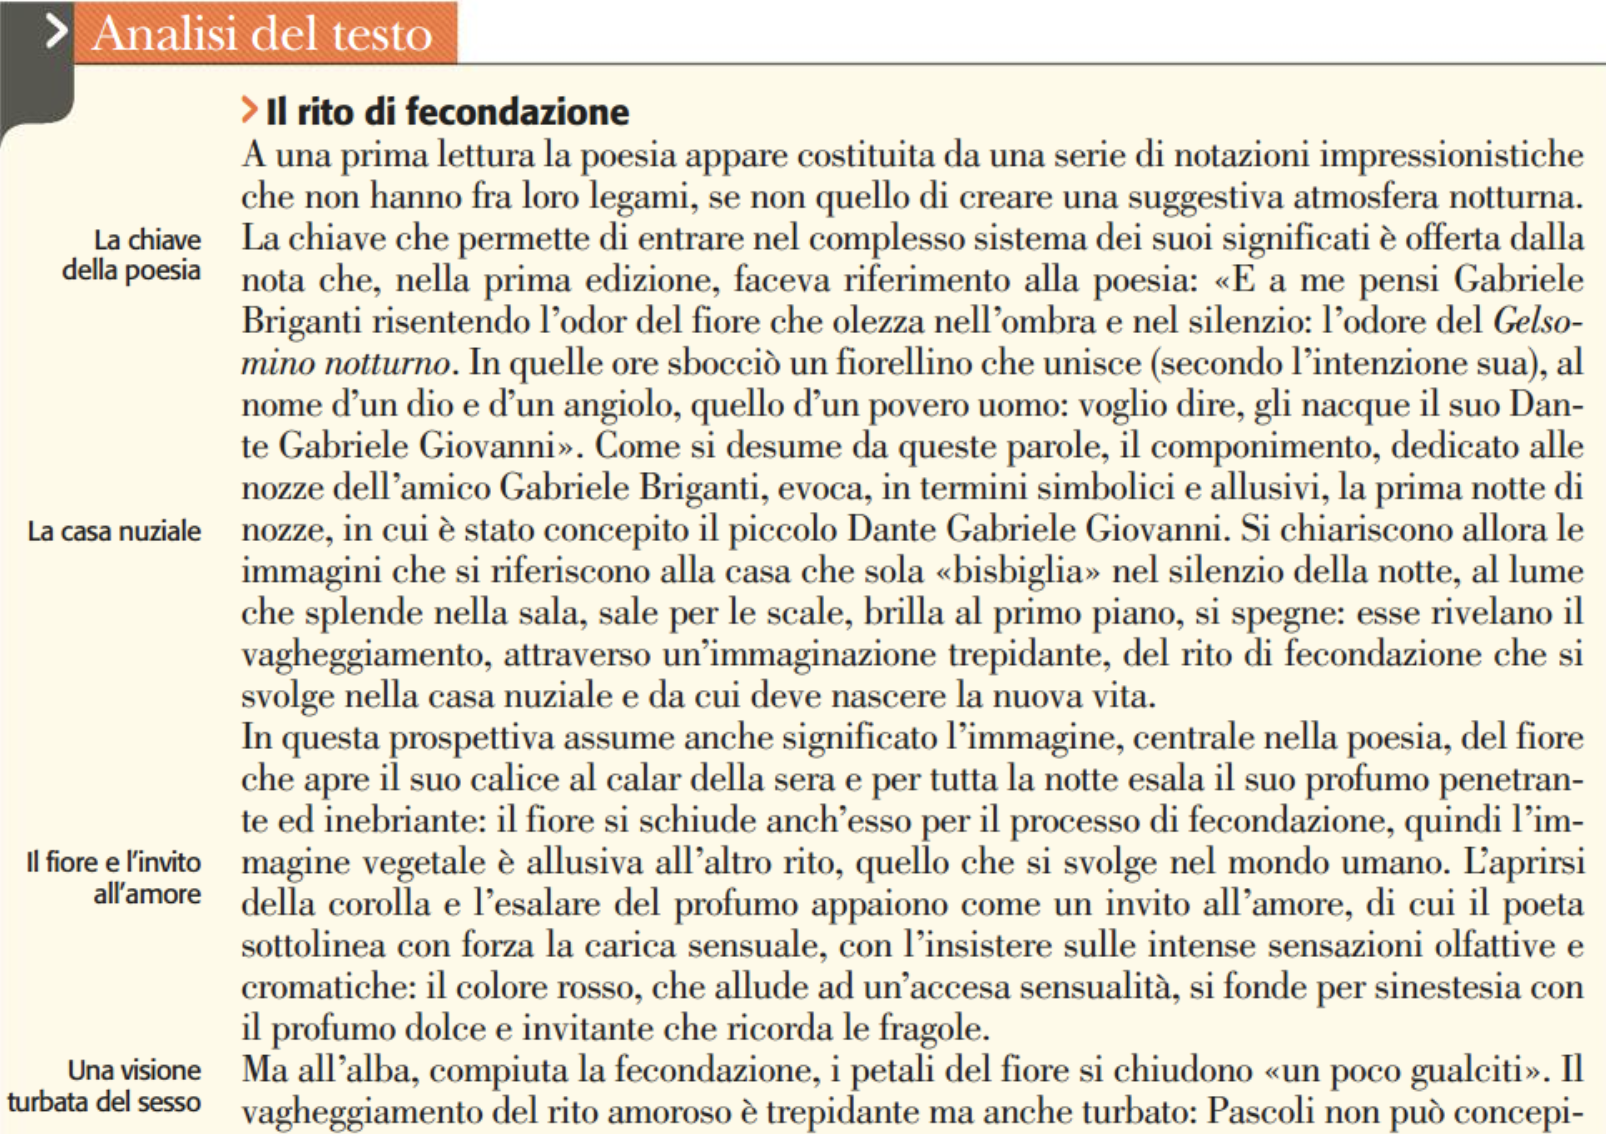
\includegraphics[width=\textwidth]{gelsomino1}
\end{center}
\vfill
\begin{center}
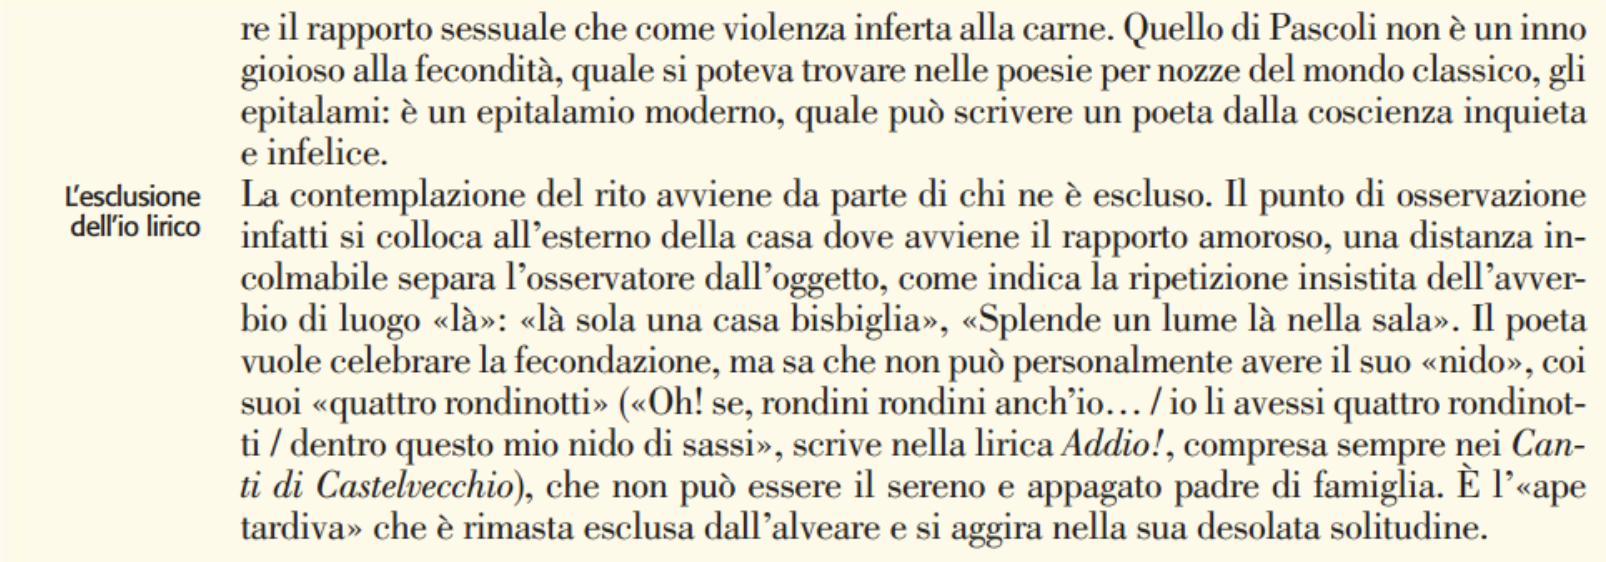
\includegraphics[width=\textwidth]{gelsomino2}
\end{center}

\begin{center}
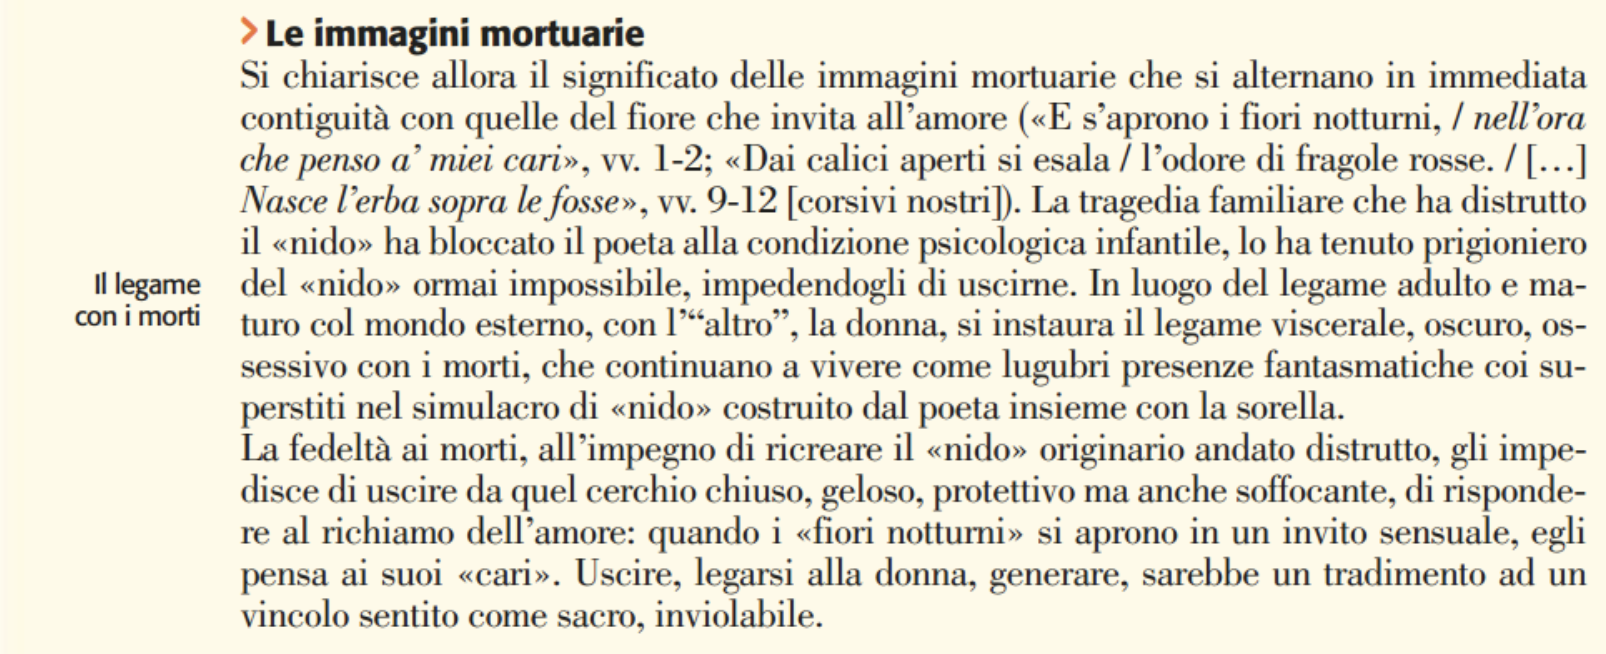
\includegraphics[width=\textwidth]{gelsomino3}
\end{center}

\begin{center}
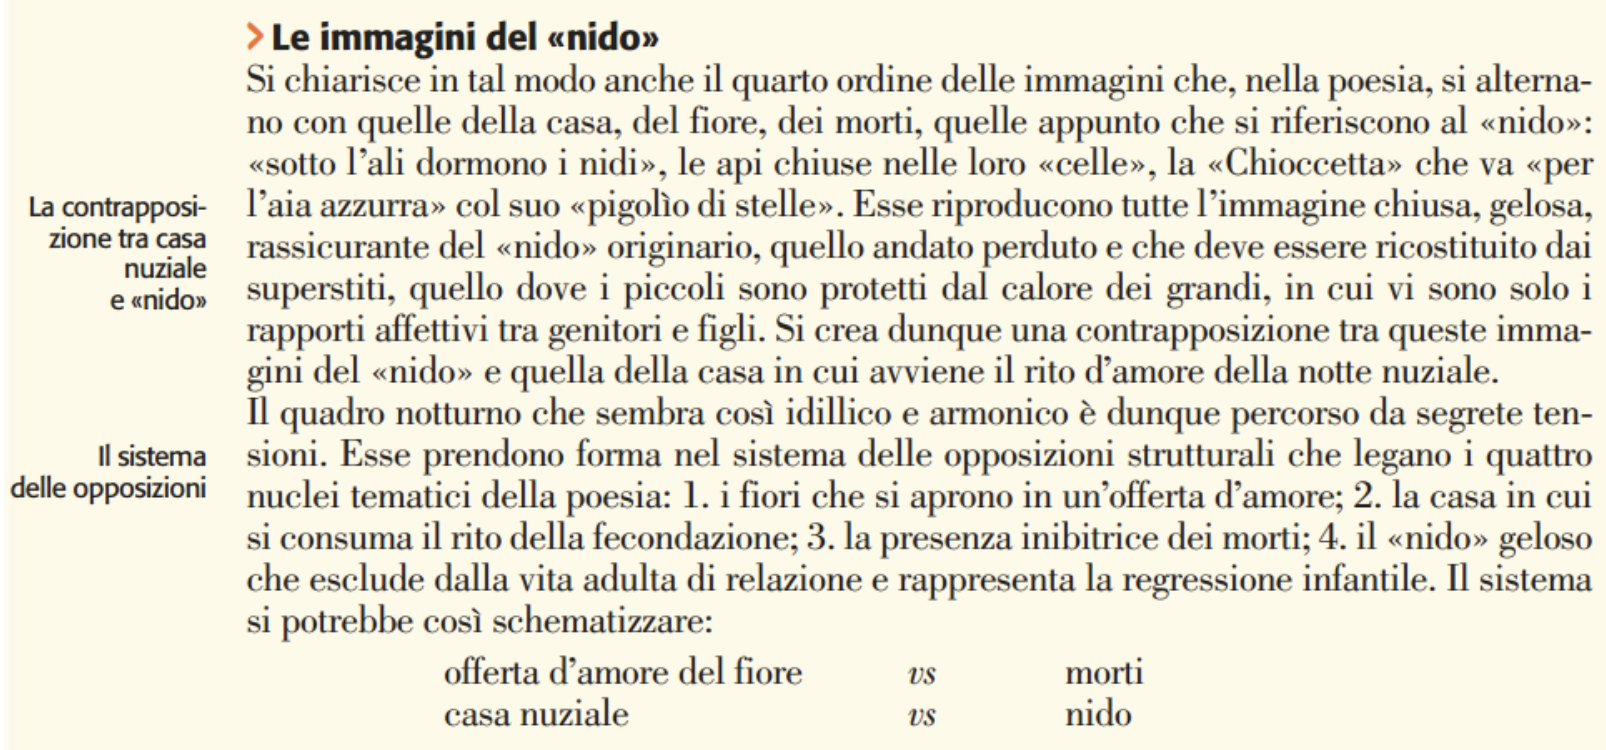
\includegraphics[width=\textwidth]{gelsomino4}
\end{center}

\begin{center}
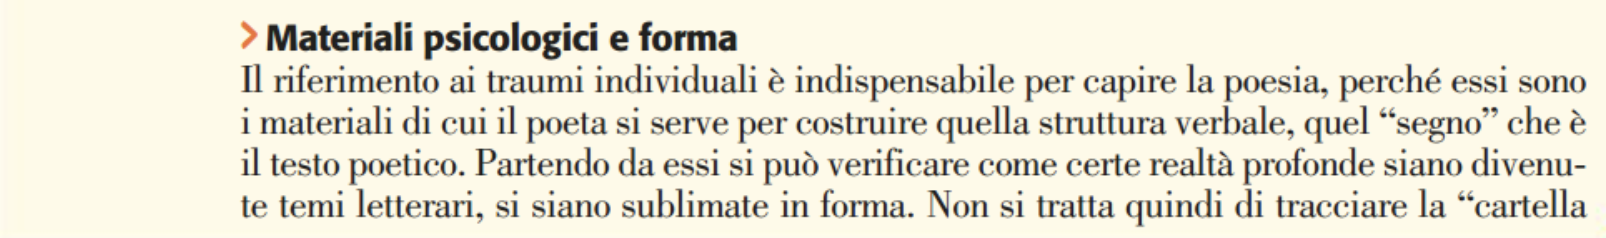
\includegraphics[width=\textwidth]{gelsomino5}
\end{center}
\vfill
\begin{center}
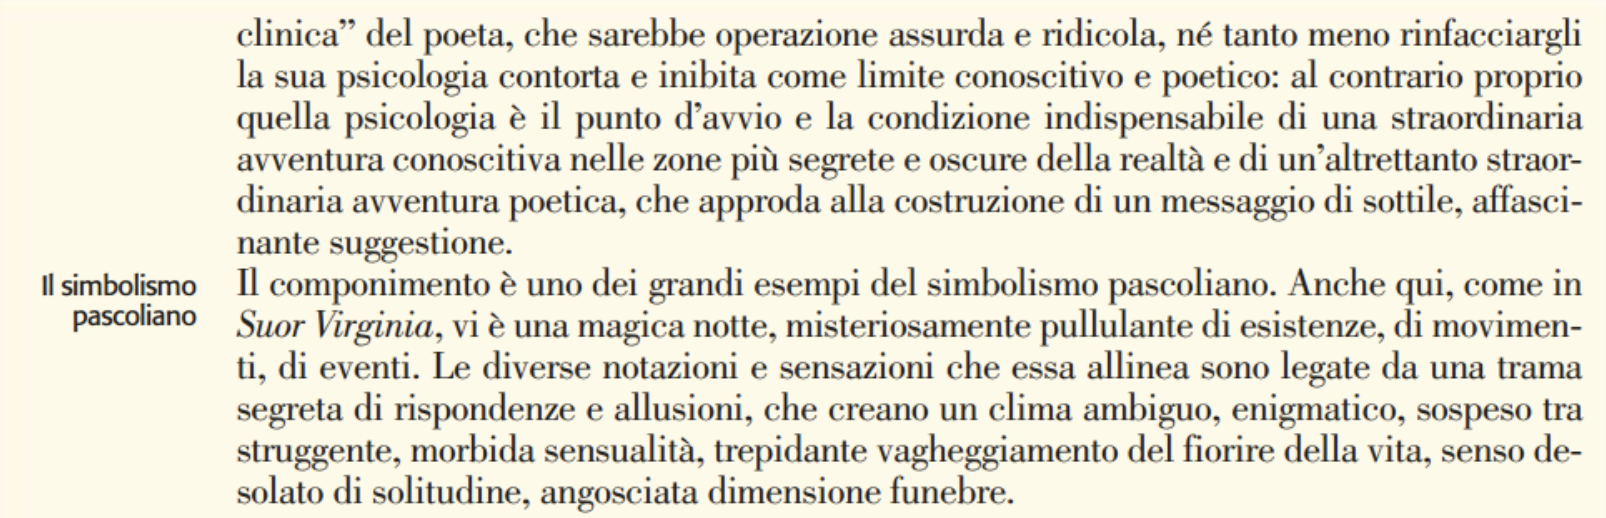
\includegraphics[width=\textwidth]{gelsomino6}
\end{center}

\part{Svevo}

\chapter{Introduzione e caratteri generali}

\elenco{\item \emph{p. 760}}

Nasce nel 1861, e la sua opera più importante (\textit{La coscienza di Zeno}) è del 1923.
Ha vissuto diverse esperienze significativo.

È un romanziere decisamente moderno. Insieme a Pirandello è il primo scrittore ad affrontare in modo sistematico il romanzo psicologico.

Ciò non significa che prima ci siano romanzi con uno scavo psicologico significativo, ma quando si parla di romanzo psicologico parliamo di un romanzo che si concentra sull'interiorità, in modo sistematico, e alla luce degli studi legati all'invenzione della psicoanalisi (sono anni di Freud). Anche dal punto di vista degli strumenti narrativi, si serve degli strumenti dati dalla psicoanalisi.

L'\textbf{inetto} è prima di tutto il disgregarsi dell'immagine maschile che corrisponde all'uomo forte, con certezze, all'eroe di tanti romanzi precedenti.
È un anti eroe, ovvero un personaggio che non ha alcuna certezze: è una forte allusione alla perdita di certezze dello scrittore e dell'intellettuale.
Non a caso i personaggi di Svevo sono spesso artisti mancati, o sono vicini al mondo artistico letterario.

L'inettitudine è un tipo di atteggiamento generale, che significa \textit{In aptus}, inadatto, incapace.
Questo concetto è molto ambiguo nella \textit{Coscienza di Zeno}, perché Zeno paradossalmente si rivelerà essere un uomo di grande successo.

\textit{La Coscienza di Zeno} è, nella finzione, la pubblicazione dello scritto-diario del protagonista, Zeno stesso.

Anche in passato, nella letteratura romantica, i personaggi sono finiti miseramente, con un suicidio. Tutti questi personaggi però avevano aspirazioni titaniche, e poi hanno fallito; l'inetto non prova nulla di tutto ciò

Per la prima volta ci troviamo di fronte ad un autore che non poggia la sua opera su basi riferite alla tradizione classica. La formazione di Zeno è \textit{sui generis}, in quanto fu avviato a degli studi tecnici dal padre.
A Trieste vi era una ricca e forte borghesia, e questa era la strada immaginata dal padre per Svevo.

Nel corso della sua vita, Svevo leggerà i classici italiani, però non c'è traccia di ciò nella sua opera. Alcuni critici ritengono che la lingua di Svevo sia imperfetta, in quanto Trieste era una città in cui si parlavano due lingue, il tedesco e l'italiano: Svevo molto probabilmente si forma maggiormente su scrittori Tedeschi, e studia l'italiano quasi come una lingua straniera; questo aspetto si ripercuote sulla lingua di Svevo, che molti ritengono imperfetta.
In realtà questa imperfezione è una scelta ben precisa

Il narratore qui è significativo: sostanzialmente il passaggio dal narratore che parla in terza persona ad un narratore che parla in prima persona. Essendo il romanzo psicologico lo studio dell'interiorità del personaggio, solo il personaggio stesso può descrivere la propria coscienza.

Il narratore però è inattendibile, perché soprattutto in Svevo egli cerca di ricomporre quegli aspetti legati alla sua coscienza che lo portano a contraddizioni, inganni. Nella \textit{Coscienza di Zeno} il dottor S ci dice proprio che Zeno è un bugiardo. Non abbiamo però punti di riferimento per capire quando il protagonista mente, etc etc etc. L'immagine che ne nasce è quella di un uomo che non ha più riferimenti nella realtà.

\section{Biografia}

La biografia dell'autore è molto importante: non succedono cose straordinarie, ma sono importanti perché ci permettono di capire il suo rapporto con la letteratura.

Abbiamo visto molti intellettuali che vivono un disagio perché non si riconoscono nei valori della società borghese. Qui l'autore, ad un certo punto della sua vita, incarna proprio la figura sociale del borghese arrivato economicamente; è come guardarsi dal di fuori, in quanto anche Svevo stesso vive il disagio dell'intellettuale.
Ad un certo punto Svevo dirà addio alla letteratura, per "risolvere il conflitto".

Svevo nasce nel 1861, da genitori ebrei, e appartiene ad una famiglia borghese. Il padre lo avvia agli studi tecnici, che gli permettano di entrare subito nel mondo del lavoro.
Nel giovane Svevo nasce subito una passione per la letteratura: per quanto non abbia fondato la sua formazione culturale sui classici, e attraverso studi canonici, egli si avvicinò autonomamente, soprattutto a scrittori tedeschi, iniziando a scrivere qualcosa.

Negli anni '80, quando Svevo aveva 18 anni, c'è il \textbf{fallimento del padre}: implica una serie di scelte, come quella di andare a lavorare in una banca, e soprattutto il \textit{declassamento sociale}, e di conseguenza economico; questo è un elemento fondamentale, che avrà delle conseguenze estremamente gravi.

Dopodiché, nel '92 Svevo scrive il suo primo romanzo: \textit{Una vita}.
Ci sono delle figure significative, in quanto il protagonista è un inetto.
Il romanzo non ha successo, e a posteriori possiamo dire che l'idea di Svevo di abbandonare la letteratura, nel 1902, sia data dal fallimento di tutte le sue opere.

Inizialmente l'attività in banca lo distoglie dagli interessi letterari: ci lavora circa 20 anni, di un lavoro arido, che egli vive con una certa indifferenza.
Nel '96 avviene il matrimonio con una lontana parente (si conoscono ad un funerale), che appartiene ad una famiglia estremamente facoltosa.
Il matrimonio è il momento della pienezza nella cultura borghese, oltrepiù significò anche poter riacquistare nella società un peso economico importante.

Grazie alla ditta dei suoceri, egli dovette viaggiare molto, e imparare l'inglese. Il suo maestro sarà proprio \textbf{James Joyce}, che diventerà suo amico e che farà conoscere il suo romanzo \textit{La coscienza di Zeno}.

Egli abbandonerà la scrittura nel 1902:
\citazione{Io, a quest'ora e definitivamente, ho eliminato dalla mia vita quella ridicola e dannosa cosa che si chiama letteratura}

Sicuramente l'insuccesso delle sue opere lo porterà lontano dalla letteratura per parecchio tempo.

Insieme alla conoscenza di Joyce, Svevo fece anche un'altra conoscenza, ovvero quella delle idee di Freud e delle sue opere.
In molti incontri in cui Svevo prese la parola, egli si espresse proprio nei confronti della psicoanalisi, che probabilmente conosceva bene.

In termini medici Svevo non era convinto dalla psicoanalisi, ma quello che Freud aveva offerto agli scrittori era ineguagliabile: la psicoanalisi per lui fu utilissima agli scrittori, perché forniva una serie di strumenti di indagine preziosissimi per scrivere romanzi psicologici.

Lo stesso Pirandello dice di non conoscere Freud, ma chiaramente le sue idee ebbero influenza su di lui.

Svevo sarà molto influenzato da alcuni pensatori, come Darwin, Nieztche, Schopenauer, Marx, spesso in antitesi tra di loro, ma prendendo da ciascuno di essi dei determinati aspetti utili alla sua letteratura.

Nel 1923 egli pubblicherà \textit{La Coscienza di Zeno}. Soprattutto in Italia ci fu una certa diffidenza nei confronti di Svevo. Fu poi Montale che scrisse una presentazione gratificante, nella rivista che dirigeva, che permise la conoscenza e l'apprezzamento di Svevo in Italia.

All'estero ebbe un grandissimo successo, soprattutto in Francia, dove l'opera fu presentata da Joyce.

Egli muore nel 1928: egli stava ritornando da una vacanza, ed ebbero un incidente di scarsa identità. Lui si ruppe in femore, e il giorno dopo morì per un enfisema polmonare, dovuto soprattutto alle sue 60 sigarette al giorno.

Egli in una nota definisce la sua vita come "non bella". Questo significa che Svevo biograficamente prende le distanze da quelli che sono stati gli interessi principali di D'Annunzio.
Egli non avrà alcun affanno nel costruire una immagine di sé, sarà distantissimo dal superuomo e dall'esteta, distantissimo da qualsiasi altro tipo di intellettuale precedenti, come la \textit{Bohemiene}. Questo si riflette sui personaggi, che sono individui assolutamente normali, alle prese con vicende normali.

Svevo era nato a \textbf{Trieste}: le sue posizioni in relazione alla posizione di Trieste furono quelle di irredentismo: all'epoca in cui Svevo visse a Trieste, questa era una città molto particolare: era multietnica, sotto il dominio austriaco, e vi era la presenza slava e italiana. Lo stesso "Italo Svevo" era uno pseudonimo per \textbf{Aron Hector Schmitz}, e ciò ci mostra la sua volontà di giungere ad una unione tra le sue due appartenenze italiana e tedesca

Si parla di cultura mittleeuropea, in quanto Trieste era di cultura molto aperta. Era stato inaugurato un porto che rappresentava per gli austriaci l'unico sbocco sul mare.

\section{Psicoanalisi}

\elenco{\item approfondimento \emph{p. 844}: Svevo e la psicoanalisi; leggere e confrontare con gli appunti}

È la scoperta dell’inconscio, qualcosa di ancora più nascosto dell’interiorità.
Quando si parla di letteratura fantastica, si dice che essa nasca quando l’uomo si rende conto che non tutto si può spiegare con la scienza. Si mettono in luce tutte quelle zone d’ombra della psiche.
Freud va a studiare queste cose con approccio scientifico, egli infatti era laureato in medicina.
L’inconscio è la parte interna dell’individuo che ha vita propria, che non può essere controllata da nessuno. Questo è destabilizzante, la crisi della personalità nasce da qui.
Il momento in cui la nostra ragione non riesce a controllare le nostre pulsioni è nel sonno.
I suoi studi parte dalla ricerca per la cura alla nevrosi. Si stabilisce un rapporto tra la malattia e la possibilità dell’individuo di descriverla e capirne le origini, la malattia diventa uno strumento conoscitivo:

\elenco{\item \textbf{Lapsus freudiano}
\item \textbf{Es}: impulsi, nel bambino e negli animali troviamo la completa espressione di questa parte di inconscio. Il bambino non se ne vergogna.
\item \textbf{Superio}: serie di norme comunemente accettate e non, come decenza, etica, morale, leggi, che vanno a controllare l’Es
\item \textbf{Io}: sta al centro tra i due, serve a bilanciarli. l’individuo è in salute ed equilibrato se l’io “fa bene il suo lavoro”, differentemente si va in nevrosi, ed è qui che entra in scena lo psicanalista.
}

La scoperta della psicoanalisi è un approccio di tipo scientifico per spiegare qualcosa che sembra sfuggire alla ragione. La psicoanalisi ha portato alla scoperta dell'inconscio, che va a creare una crisi di personalità dell'individuo, in quanto quando egli scopre che c'è una parte di sé su cui non ha alcun controllo emerge un aspetto inquietante.

L'intervento della psicoanalisi serve a riportare alla luce alcuni elementi che possono essere definiti parte dell'inconscio, come desideri e traumi, che sono stati messi a tacere.

Insieme a questo tentativo di portare in equilibrio l'individuo, definito nevrotico se l'\textit{es} e il \textit{superio} non è equilibrato correttamente dall'\textit{io}: a questo punto ha bisogno della psicoanalisi

Svevo non aveva fiducia nella psicoanalisi come terapia medica, ma proprio dalla psicoanalisi egli riesce ad ottenere gli strumenti di indagine che gli permettono di scavare nei suoi personaggi.

Nella terapia psicoanalitica un elemento fondamentale è il sogno è quel momento in cui non c'è nessun controllo della ragione, per cui una sua eventuale analisi ci permette di scoprire qualcosa dell'inconscio.

Ci sono molti altri elementi, come i lapsus, gli atti mancati, la gestualità del corpo, in cui l'inconscio prende il sopravvento.

Un esempio di atto mancato ne \textit{La Coscienza di Zeno} è quando lui si dimentica di andare al funerale del cognato.
L'atto mancato è un qualcosa che viene meno rispetto la volontà dell'individuo. Nel caso di questo episodio Zeno si dimentica di andare al funerale del cognato. Per Freud questo è un chiaro atto mancato, che va spiegato in questi termini: l'inizio del rapporto tra Zeno e Guido è conflittuale, in quanto quest'ultimo è un protagonista forte e vitale, che tende a contrapporsi all'inetto; poi diventano soci in affari e grandi amici, però probabilmente nell'inconscio di Zeno questa antipatia e questa avversione per Guido resta, tanto che quando quest'ultimo muore Zeno si dimentica di andare al funerale.

Svevo dice
\citazione{Grande uomo quel nostro Freud, ma più per i romanzieri che per gli ammalati. \textit{Letterariamente} certo Freud è più interessante. Magari avessi fatto io una cura con lui. Il mio romanzo sarebbe risultato più intero. E perché voler curare la nostra ? Davvero dobbiamo togliere all'umanità quello ch'essa ha di meglio? Io credo sinceramente che il vero successo che mi ha dato la pace è consistito in questa convinzione.}

Svevo inizia ad avvicinarsi alla psicoanalisi nel 1908, che è abbastanza presto per l'epoca. Insieme ad un suo nipote egli cerca di tradurre i primi scritti di Freud sul sogno.
Egli aveva avuto rapporti con un collaboratore di Freud, nel 1910-11.

Il cognato di Svevo, molto più giovane di lui, era un giovane omosessuale tossicodipendente, che i genitori avevano affidato alle cure di Freud. Ci sono delle lettere in cui Svevo racconta questa esperienza, con l'assoluta mancanza di riscontro della terapia, in quanto il cognato venne distrutto alla fine della terapia.

Nel linguaggio di Freud, l'esperienza di Svevo è una sorta di resistenza: la resistenza del paziente a volte avviene: il paziente a volte è intenzionato a difendere la propria malattia.
Questo problema non è neanche così distante da Zeno, nei confronti del fumo, che fino alla fine continuerà a fumare.
Questo vizio attanglierà anche l'autore stesso

Il fumo, all'interno del romanzo, viene talvolta interpretato come una sorta di autoinganno: lui è un inetto, e considerando che inizia la sua terapia con il tentativo di smettere di fumare, è probabile che egli si senta un inetto a causa della malattia del fumo: se poi, guarito da questa malattia, egli avesse scoperto di essere ancora un inetto, non avrebbe più potuto giustificare la sua inettitudine; di conseguenza, sembra quasi che Zeno \textit{voglia} continuare a fumare.

Svevo dice:
\citazione{E perché voler curare la nostra malattia? Davvero dobbiamo togliere all'umanità quello che essa ha di meglio?}

La presa di coscienza rispetto alla malattia è uno strumento conoscitivo.

\subsection{Malattia}

Nell’800 fa la sua comparsa in letteratura, non che prima fosse bandita, ne è un’esempio la peste che si sentì la prima volta nell’Illiade, quando la peste va a colpire l’esercito dei Greci, poi la peste di Atene, e quella del Boccaccio.

Dall’800 però arriva una malattia che fece tantissimi morti, la tubercolosi, come nella signora delle camelie, ma anche tanti autori ne furono colpiti.
Divenrta così importante perché poco  apoco divenne metafora del malessere iteriore. La malattia fisica porta con sé molte immagini evocative, come il pallore della donna ammalata che ci riporta al pallore delle donne cantate partendo dalla lirica provenzale, la tisi porta anche altri colori come quello del sangue, il rosso ha grande valore figurativo in letteratura.

Lo troviamo anche nella scapigliatura, come la Fosca, ma anche nel naturalismo e nei personaggi di Zola. Altra malattia è l’alcolismo che miete parecchie vittime, compisce le eroine come anche i poeti poveri, vedi i bohemian.
Col decadentismo la malattia diventa l’espressione del “cupio (desidero) dissolvio (distruzione)”, è quindi il desiderio dell’autodistruzione.
La malattia di Zeno è il disadattamento, ci sono anche riscontri fisici, la malattia dell’anima diventa malattia fisica. Questo è il filo portante della coscienza di Zeno

\subsubsection*{\href{https://www.corriere.it/cultura/eventi/2013/scala/notizie/malattia-destino-ineluttabile-cosi-tisi-consumo-l-ottocento-42b66182-5e85-11e3-aee7-1683485977a2.shtml}{Approfondimento}\footnote{https://www.corriere.it/cultura/eventi/2013/scala/notizie/malattia-destino-ineluttabile-cosi-tisi-consumo-l-ottocento-42b66182-5e85-11e3-aee7-1683485977a2.shtml}}

«La contessina Bice spegnevasi lentamente. Di malattia di languore, dicevano gli uni. Di mal sottile, dicevano gli altri», scrive Giovanni Verga nella novella Dramma intimo, tracciando (involontariamente) una breve storia ragionata della tubercolosi: per tutto l’Ottocento e per buona parte del Novecento, ha colpito ricchi e poveri, cancellando molte linee di confine tra le classi sociali ma, mentre i meno abbienti esibivano il pallore con rassegnazione secolare, i borghesi dissimulavano. Nascondevano. Seppellivano.

Perché la tisi era la malattia dei poveri, delle prostitute (un contrappunto all’altrettanto temutissima «malattia romantica», la sifilide). Ed è stata la patologia letteraria che maggiormente ha sfinito le peccatrici, come, appunto, Violetta de «La traviata» o, per restare nella lirica, Mimì de «La Bohème». Contrappasso (narrativo) che ha del sottile: il rosso del peccato da una parte e il rosso del sangue come punizione. Su pelle bianchissima, come quella esangue di Lisbeth, ossia la «cugina Bette» dell’omonimo romanzo di Honoré de Balzac, la quale verrà colpita dalla tubercolosi in un mondo che, se possibile, è ancora più marcio della malattia: rancori, erotomani, parenti vendicatori, veleni familiari. Sì, perché il romanzo realista ottocentesco ha spesso incastonato la tisi in un universo di per sé vizioso, come se questa fosse l’apoteosi della perdizione, lo sguardo sull’abisso dei pittori romantici, l’ultimo atto di un mondo estremo e stremato.

Soffrono di tisi i personaggi stremati à la Émile Zola, che nei suoi assommoir riversa le viscere febbricitanti di una periferia parigina malsana, malata, in definitiva: condannata. Condannata a essere sfruttata in miniera, a oliare la macchina del progresso, a preparare la strada del secolo breve (alla peccaminosa Nanà, però, Zola assegnerà una morte simbolica: il vaiolo le sfigurerà il viso gonfio di vizi). Si consumano le donne e gli uomini che Maupassant incrociava nelle sue passeggiate in quel di Cannes.

\begin{figure}
\centering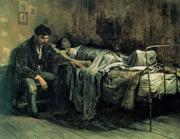
\includegraphics[width=4cm]{3}
\caption{«La miseria» (1886), olio dello spagnolo Cristóbal Rosas}
\end{figure}

Si consumano le borghesi di Tolstoj, come la signora tisica che nella novella Tre morti intraprende un ultimo viaggio verso climi più miti. Si consumano gli stessi artisti, come Cechov, che nel giardinaggio trovava riposo e cercava di curarsi; come Chopin, tisico dichiarato, che ebbe non pochi problemi nell’affrontare viaggi all’estero; come Kafka, che si macerava nel corpo e nello spirito, mangiato da una malattia che minava la sua esistenza e il suo alfabeto amoroso; come Emily Brontë, che se n’è andata giovane; come Keats, e Pergolesi, e Orwell e Gozzano. Guido Gozzano, sì, quello che ci ha regalato una delle pagine più struggenti sul mal sottile: «Mi picchiano in vario lor metro spiando non so quali segni,/ m’auscultano con li ordegni il petto davanti e di dietro./ E senton chi sa quali tarli i vecchi saputi... A che scopo? /Sorriderei quasi, se dopo non bisognasse pagarli...».

Epperò, inseguendo una specie di attrazione fatale che nell’Ottocento lega la donna alla morte (si legga, a questo proposito, La morte ci fa belle, di Francesca Serra, edito da Bollati Boringhieri) la tubercolosi donava alle donne un pallore quasi lunare, un’evanescenza che era pressoché un riscatto dei piaceri carnali nei quali avevano diluito la giovinezza. Tremavano di una bellezza non dicibile, languivano. E anche Leopardi, con la sua Silvia, contribuisce a far conoscere il «chiuso morbo».

Nell’introduzione al volume Il morbo lento. La tisi nell’Italia dell’Ottocento (Franco Angeli) di Eugenia Tognotti, Giorgio Cosmacini riporta una frase del medico condotto di Sondalo (in provincia di Sondrio) Ausonio Zubiani: «Vi sono due tisi, quella dei ricchi che qualche volta guarisce e quella dei poveri che non guarisce mai». Come a voler delineare, stavolta, una demarcazione netta tra quelli che pagano colpe proprie (il peccato) e quelli che scontano un destino scritto.

Infine, nel Novecento, la tisi si manifesterà in simboli molto diversi. In Thomas Mann, la tubercolosi (e anche altre malattie) non sarà più viste tanto come un destino dell’uomo, bensì come una condizione esistenziale. La modernità è anche un riconoscere la propria parte malata, uno scavo nel corpo che somatizza in un moto dello spirito. Nel sanatorio di Davos, la clinica Berghof (nome di fantasia), Mann ambienta La montagna incantata, sintesi dell’uomo novecentesco, stretto in un perimetro claustrale, quasi costretto a guardarsi dentro, a sezionare le proprie ferite. Va detto che nel 1920 erano 80mila i reduci tedeschi ammalati di tubercolosi il romanzo è stato pubblicato nel 1924.

Del 1981 è invece \titolo{La diceria dell’untore}, romanzo d’esordio di Gesualdo Bufalino, dove Marta, una giovane ammalata di tisi, perde quella carica quasi erotica dei personaggi di Mann per diventare emblema di un mondo in dissoluzione. Anche la malattia ha un suo percorso, dunque, e la letteratura lo segue fino in fondo.


\chapter{\textit{Una vita}}
\elenco{\item \emph{p. 770-773}}

È la storia di un giovane, Alfonso Nitti, che abbandona il paese e la madre per venire a lavorare a Trieste, dopo che la morte del padre, medico condotto, ha lasciato la famiglia in ristrettezze. Si impiega presso la banca Maller, ma il lavoro gli appare arido e mortificante. Il giovane, imbevuto di letteratura, orgoglioso della sua cultura umanistica, evade costruendosi «sogni da megalomane» e vagheggiando la gloria letteraria.
L'occasione per un riscatto dalla sua vita vuota e solitaria, riempita solo dalle avide letture presso la biblioteca comunale, gli è offerta da un invito a casa del padrone della banca, Maller. Alfonso conosce così Macario, un giovane brillante e sicuro di sé, e stringe con lui una forma di amicizia. In Macario l'eroe, nella sua provinciale goffaggine e timidezza, trova una sorta di appoggio e di modello. La figlia di Maller, Annetta, ha anch'essa ambizioni letterarie e sceglie Alfonso come collaboratore nella stesura di un romanzo. Alfonso, pur senza amare Annetta, la seduce e la possiede. A questo punto l'eroe avrebbe la possibilità di trasformare radicalmente la propria vita, sposando la ricca ereditiera. A tale soluzione è spinto insistentemente dalla signorina Francesca, istitutrice in casa di Maller e sua amante, che aspira anch'essa al salto di classe attraverso il matrimonio con il padrone. Alfonso invece, preso da un'inspiegabile paura, fugge da Annetta e da Trieste, adducendo come pretesto una malattia della madre.

Tornato al paese, trova effettivamente la madre gravemente ammalata. Dopo la sua morte ritorna di nuovo a Trieste, deciso a rinunciare alla crudele «lotta per la vita che domina nell'ambiente in cui vive, credendo di aver scoperto nella rinuncia e nella contemplazione la sua vera natura (si rivela in questo l'influenza di Schopenhauer, il filosofo amato da Svevo, \textit{I maestri di pensiero: Schopenhauer, Nietzsche, Darwin}, \emph{p. 766}). Ma la realtà smentisce le belle teorie e i nobili programmi. Alfonso credeva di aver interamente superato le passioni, invece, all'apprendere che Annetta, sdegnata con lui, si è fidanzata con Macario, è invaso da una dolorosa gelosia; riteneva di non curarsi più del giudizio degli altri, ed invece si sente ferito dal disprezzo e dall'odio che lo circonda nella banca.

Trasferito ad un compito di minore importanza, affronta indignato il signor Maller, ma nell'emozione si lascia sfuggire frasi che vengono interpretate come ricatti. Da questo momento commette errori irreparabili: scrive ad Annetta per chiederle che cessing le persecuzioni nei suoi confronti, ma di nuovo il suo gesto è avvertito dai Maller come ricattatorio. All'appuntamento che egli ha chiesto alla ragazza, per una definitiva spie gazione, si presenta il fratello, che lo sfida a duello, Alfonso, sentendosi «incapace alla vita», decide di cercare nella morte una via di scampo, il mezzo per divenire «superiore ai sospetti e agli odi», distruggendo la fonte della sua infelicità, il suo organismo «che non conosceva la pace».

\section{T: \textit{Le ali del gabbiano}}
\elenco{\item \emph{p. 773}}

\setcounter{mar}{0}
\begin{quotation}
La sua compagnia doveva piacere a Macario. La cercava di spesso; qualche sera gli usò anche la gentilezza di andarlo a prendere all’ufficio.

Ad Alfonso non sfuggì la causa di quest’affetto improvviso. Lo doveva alla sua docilità e, pensò, anche alla sua piccolezza. Era tanto piccolo e insignificante, che accanto a lui Macario si trovava bene. Non si compiacque meno di tale amicizia. Le cortesie, anche se comperate a caro prezzo, piacciono. Non disistimava Macario. Per certe qualità ammirava quel giovine tanto elegante, artista inconscio, intelligente anche quando parlava di cose che non sapeva.

Macario possedeva un piccolo cutter e frequentemente invitò Alfonso a gite mattutine nel golfo. Nella sua vita triste, quelle gite furono per Alfonso vere feste. In barca gli era anche più facile di dare il suo assenso alle asserzioni di Macario e in gran parte non le udiva. Si trovava ancora sempre alla conquista della solida salute che gli occorreva, riteneva, per sopportare la dura vita di lavoro a cui faceva proponimento di sottoporsi, e gli effluvi marini dovevano aiutarlo a trovarla.

Una mattina soffiava un vento impetuoso e alla punta del molo, ove si trovavano per attendere la barca che doveva venirli a prendere, Alfonso propose a Macario di tralasciare per quella mattina la gita che gli sembrava pericolosa. Macario si mise a deriderlo e non ne volle sapere.

Il cutter si avvicinava. Piegato dalle vele bianche gonfiate dal vento, sembrava ad ogni istante di dover capovolgersi e di raddrizzarsi all’ultimo estremo sfuggendo al pericolo imminente. Alfonso da terra era colto da quei tremiti nervosi che si hanno al vedere delle persone in pericolo di cadere e fu solo per la paura delle ironie di Macario che non seppe lasciarlo partir solo.

Ferdinando, un facchino ch’era stato marinaio, dirigeva la barca. Lasciò il posto al timone a Macario il quale sedette dopo toltasi la giubba quasi per prepararsi a grandi fatiche:

— Ora fuoco alla macchina, — gridò a Ferdinando.

Ferdinando scese a terra e trascinò il cutter per l’albero di prora da un angolo del molo all’altro; poi, un piede puntellato a terra, l’altro sul cutter, lo spinse al largo.

Alfonso lo guardò tremando; temeva di vederlo piombare in acqua\mat{paura per sé e per gli altri} e, per quanto piccolo, l’imminenza di un pericolo lo faceva sussultare.

— Che agile! — disse a Ferdinando.

Gli pareva d’essere in mano sua e aveva il desiderio quasi inconscio d’amicarselo. Ferdinando alzò il capo, giovanile ad onta del grigio nella barba e della calvizie abbastanza inoltrata, e ringraziò. Non essendo suo il mestiere, ci teneva molto ad apparire abile. Comprese però male lo scopo della raccomandazione. Trasse con forza a sé la vela e la fissò, aiutando poscia a tenderla con tutto il peso del suo corpo. Immediatamente il vento che pareva sorgesse allora la gonfiò e la barca si piegò con veemenza proprio dalla parte ove sedeva Alfonso.

S’era proposto di far mostra di grande sangue freddo, ma i propositi non bastarono all’improvviso spavento.\mat{l'inetto non è capace, vorrebbe mostrare sangue freddo ma non riesce, tanto che suscita una reazione ironica da parte dell'antagonista } Poté trattenersi dal gridare ma balzò in piedi e si gettò dall’altra parte sperando di raddrizzare la barca con il suo peso. Si tranquillò alquanto sentendosi più lontano dall’acqua e sedette afferrandosi con le mani alla banchina.

Macario lo guardò con un leggero sorriso. Si sentiva bene nella sua calma accanto ad Alfonso e per rendere più evidente il distacco tenne il cutter sotto la piena azione del vento.\mat{fa dei tentativi, non riusciti} Alfonso vide il sorriso e volle prendere l’aspetto di persona calma. Segnalò a Macario all’orizzonte delle punte bianche di montagne di cui non si vedevano le basi.

Passando accanto al faro poté misurare la rapidità con la quale tagliavano l’acqua; diede un balzo sembrandogli che la barca andasse a sfracellarsi sui sassi che la contornavano.

— Sa nuotare? — gli chiese Macario con tranquillità. — Alla peggio ritorneremo a casa a nuoto. Ma — e finse grande preoccupazione — anche se si sentisse andare a fondo non si aggrappi a me perché saremmo perduti in due. Penseremo a lei io e Nando. Nevvero, Nando?

Ridendo sgangheratamente, costui lo promise.

Coi suoi modi da pensatore, Macario si dilungò in considerazioni sugli effetti della paura. Ogni dieci parole alzava la mano aristocratica, l’arrotondava e tutti i sottintesi che quel gesto segnava, cui nel vuoto della mano creava il posto, Alfonso lo sapeva, dovevano andare a colpire lui e la sua paura.

— Muore maggior numero di persone per paura che per coraggio. Per esempio in acqua, se vi cadono, muoiono tutti coloro che hanno l’abitudine di afferrarsi a tutto quello che loro è vicino, — e fece una strizzatina d’occhio verso le mani di Alfonso che si chiudevano nervosamente sulla banchina.

E passarono accanto al verde Sant’Andrea senza che Alfonso potesse padroneggiarsi. Guardava, ma non godeva.

La città, quando al ritorno la rivide, gli parve triste.\mat{malattia} Sentiva un grande malessere, una stanchezza come se molto tempo prima avesse fatto tanta via e che poi non lo si fosse lasciato riposare mai più. Doveva essere mal di mare e provocò l’ilarità di Macario dicendoglielo.

— Con questo mare!

Infatti il mare sferzato dal vento di terra non aveva onde. Vi erano larghe strisce increspate, altre incavate, liscie liscie precisamente perché battute dal vento che sembrava averci tolto via la superficie. Nella diga c’era un romoreggiare allegro come quello prodotto da innumerevoli lavandaie che avessero mosso i loro panni in acqua corrente.

Alfonso era tanto pallido che Macario se ne impietosì e ordinò a Ferdinando di accorciare le vele.

Si era in porto, ma per giungere al punto di partenza si dovette passarci dinanzi due volte.

Si udivano i piccoli gridi dei gabbiani. Macario per distrarlo volle che Alfonso osservasse il volo di quegli uccelli, così calmo e regolare come la salita su una via costruita, e quelle cadute rapide come di oggetti di piombo. Si vedevano solitarii, ognuno volando per proprio conto, le grandi ali bianche tese, il corpicciuolo sproporzionatamente piccolo coperto da piume leggiere.

— Fatti proprio per pescare e per mangiare, — filosofeggiò Macario. — Quanto poco cervello occorre per pigliare pesce! Il corpo è piccolo. Che cosa sarà la testa e che cosa sarà poi il cervello? Quantità da negligersi! Quello ch’è la sventura del pesce che finisce in bocca del gabbiano sono quelle ali, quegli occhi, e lo stomaco, l’appetito formidabile per soddisfare il quale non è nulla quella caduta così dall’alto. Ma il cervello! Che cosa ci ha da fare il cervello col pigliar pesci? E lei che studia, che passa ore intere a tavolino a nutrire un essere inutile! Chi non ha le ali necessarie quando nasce non gli crescono mai più. Chi non sa per natura piombare a tempo debito sulla preda non lo imparerà giammai e inutilmente starà a guardare come fanno gli altri, non li saprà imitare. Si muore precisamente nello stato in cui si nasce, le mani organi per afferrare o anche inabili a tenere.

Alfonso fu impressionato da questo discorso. Si sentiva molto misero nell’agitazione che lo aveva colto per cosa di sì piccola importanza.

— Ed io ho le ali? — chiese abbozzando un sorriso.

— Per fare dei voli poetici sì! — rispose Macario, e arrotondò la mano quantunque nella sua frase non ci fosse alcun sottinteso che abbisognasse di quel cenno per venir compreso.
\end{quotation}

Da questo brano evinciamo con estrema chiarezza il carattere dell'inetto, che poi vedremo con delle varianti nei romanzi successivi.

Questo aspetto, cioè da una parte il suo volere e dall'altra non riuscire ad attendere questa volontà, è significativo del fatto che alla base ci sia la teoria Darwiniana e di Schopenauer

Macario, dinnanzi all'atteggiamento di Alfonso, gli spiega teoricamente qual è il problema. Svevo prende spunto da molti filosofi, tra cui Darwin e Schopenauer.

Svevo ama molto la filosofia, studia i filosofi tedeschi e non solo: ne fa un uso particolare, in quanto i filosofi sono spesso in contrasto tra di loro. Talvolta sembra difficile trovare un contatto tra alcuni di essi, perché l'atteggiamento di Svevo è "strumentale": egli trae molto spesso dai filosofi degli strumenti di analisi che gli servono per costruire i suoi personaggi.
Per esempio, per quel che riguarda Marx, a Svevo interessa non il pensiero, quanto la scoperta della lotta tra le classi, ripresa in Svevo, e che gli serve per dare una connotazione ai suoi personaggi.
Svevo stesso è andato "avanti e indietro" tra le classi sociali.

Da Schopenauer, che spesso è visto in parallelo a Leopardi, Svevo prende la teoria sugli istinti inconsci dell'essere umano, che secondo Schopenauer devono essere soppressi; gli suggeriscono il modo di tratteggiare i suoi personaggi, che sono spesso dei bugiardi: nella \textit{Coscienza di Zeno} è il dottor S che dice proprio che Zeno è un bugiardo. Il protagonista quindi è \textbf{inattendibile}. Solo il narratore, in un romanzo, può smascherare gli inganni del protagonista, sempre che questi non coincidano. Ne \textit{La Coscienza di Zeno}, coincidendo queste due figure, non è possibile smascherare le bugie. Il lettore è senza parametri per poter capire le finzioni di Zeno, per cui non si hanno più certezze. Sia in \textit{Una Vita} che in \textit{Senilità} il narratore è esterno.

In questo brano, Macario spiega la sua filosofia ad Alfonso: gli dice che uno è vincente o perdente per natura, e la lotta per la vita fa sì che i più forti vincano e i più deboli perdano. Si usa la metafora con il gabbiano, vincente per natura. Ci sono continui riferimenti al cervello, chiamato \textit{essere inutile}: dietro agli inetti di Svevo ci sono sempre intellettuali, e questo è significativo del modo in cui Svevo denuncia il malessere dell'intellettuale (situazione che vive anche sulla sua persona, in quanto egli abbandona la letteratura). Viene irriso il protagonista, in quanto pur studiando è incapace.
Si tratta di capire se c'è possibilità di attuare la volontà: no, in quanto è una \textbf{legge naturale}.
\citazione{Chi non sa per natura piombare a tempo debito sulla preda non lo imparerà giammai e inutilmente starà a guardare come fanno gli altri, non li saprà imitare. Si muore precisamente nello stato in cui si nasce, le mani organi per afferrare o anche inabili a tenere.}

L'ultima battuta è un attacco alla passione di Alfonso per la poesia.

Ancora anni più tardi in una lettera del 1927, Pirandello ribadirà, citando Schopenauer, che il contemplatore è un prodotto della natura, finito quanto il lottatore (cioè il contemplatore non è a uno stadio imperfetto della formazione umana, ma un prodotto di natura già perfettamente compiuto come lo è il lottatore). Quindi è probabile che sia d'accordo sul fatto che l'inettitudine di Alfonso sia un dato di natura

Le teorie di Macario sono giuste, in quanto Alfonso alla fine si suicida: è probabile che l'idea di Svevo sia uguale a quella di Macario.
Non si capisce perché egli affidi a Macario, personaggio negativo, la sua stessa idea.

\begin{center}
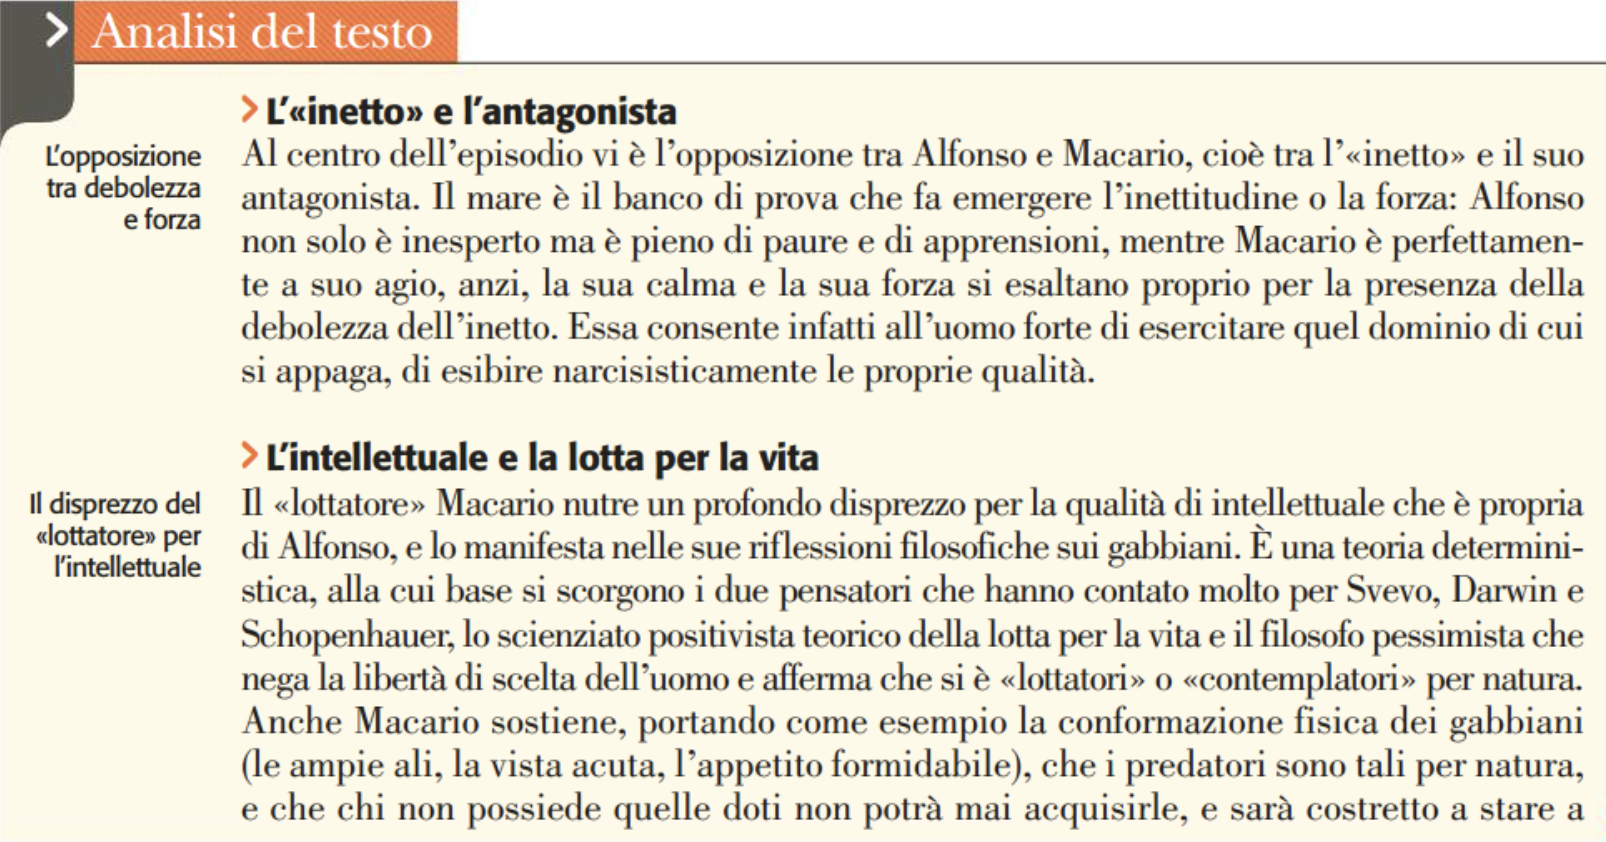
\includegraphics[width=\textwidth]{ali1}
\end{center}
\vfill
\begin{center}
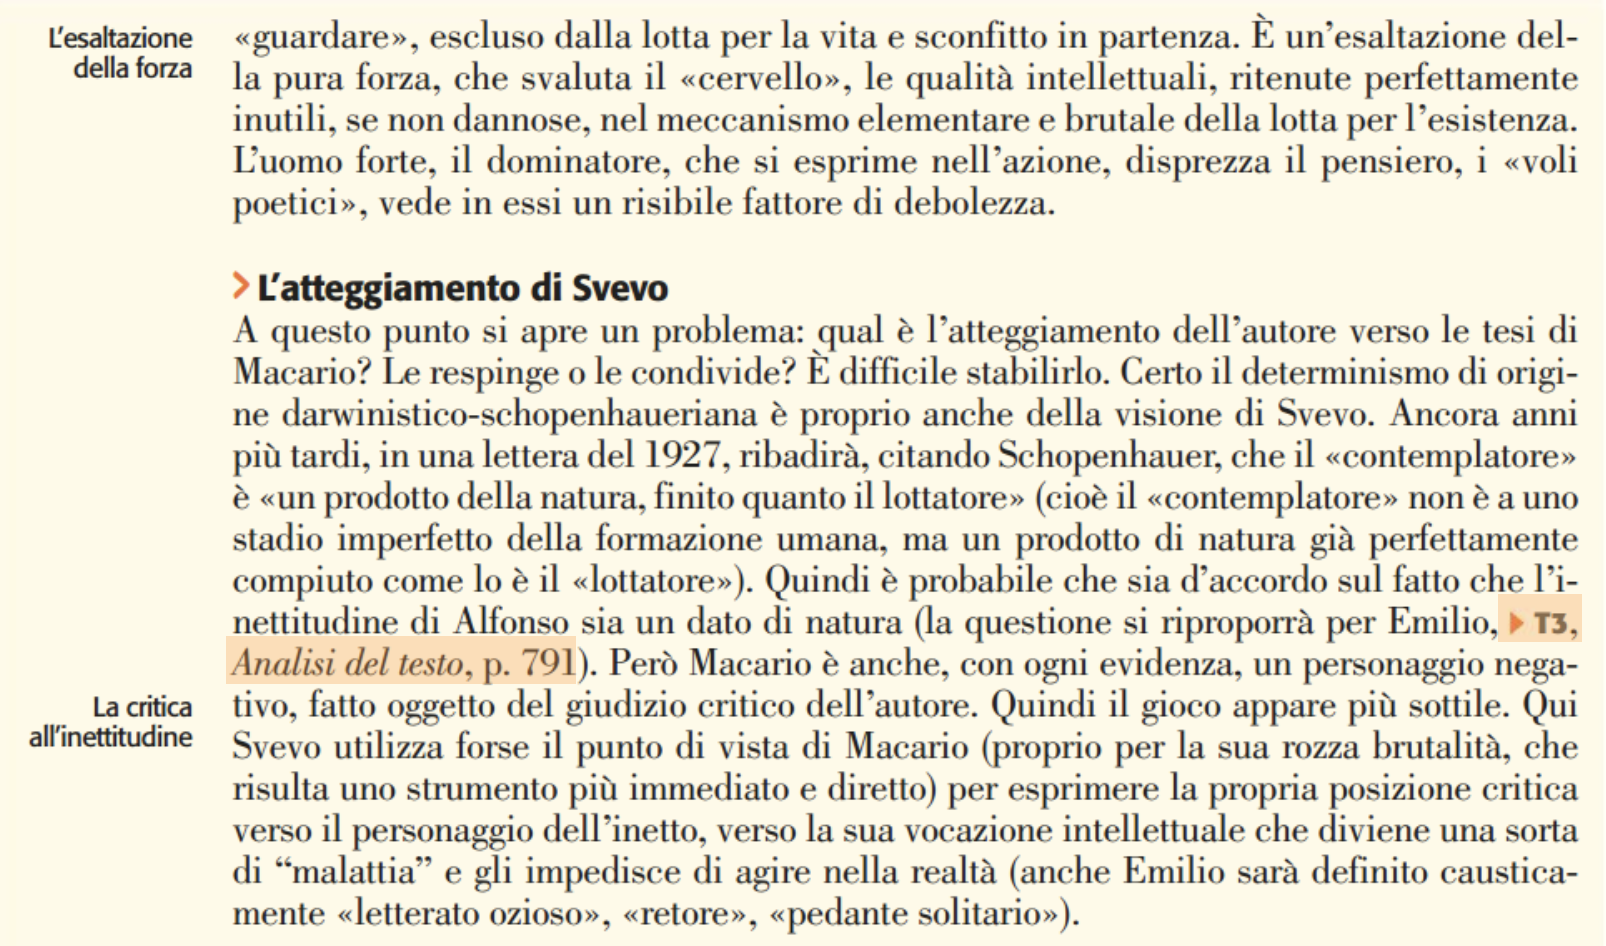
\includegraphics[width=\textwidth]{ali2}
\end{center}

\chapter{\textit{Senilità}}

\section{Trama}
Il protagonista, Emilio Brentani, trentacinquenne, vive di un modesto impiego presso una società di assicurazioni triestina e gode di una certa reputazione in ambito cittadino per un romanzo pubblicato anni prima, dopo il quale però non ha scritto più nulla. Egli ha attraversato la vita con prudenza, evitando i pericoli ma anche i piaceri, appoggiandosi alla sorella Amalia, con cui vive e che lo accudisce «come una madre dimentica di se stessa», e all'amico Stefano Balli (personaggio ispirato al pittore Umberto Veruda, amico di Svevo), scultore, uomo dalla personalità forte, che compensa l'insuccesso artistico con un'eccezionale fortuna con le donne, e che rappresenta per il debole Emilio una sorta di figura paterna. L'insoddisfazione per la propria esistenza vuota e mediocre spinge però Emilio a cercare il godimento nell'avventura, che egli crede «facile e breve», con una ragazza del popolo, Angiolina, conosciuta casualmente. Emilio si propone semplicemente di divertirsi senza impegnarsi, imitando il dongiovannismo dell'amico Balli. In realtà si innamora perdutamente della ragazza, idealizzandola e trasformandola nella sua fantasia in una creatura angelica.

La scoperta della vera natura di Angiolina, che ha numerosi amanti e si rivela cinica e mentitrice, scatena la sua gelosia, che assume veri e propri caratteri ossessivi. Ma egli non riesce a staccarsi dalla ragazza: un tentativo di separazione lo getta in uno stato di prostrazione profonda, privandolo di quella energia vitale che aveva trovato nel rapporto, e che egli definisce «gioventù». Di conseguenza riallaccia la relazione, ma il possesso fisico, a cui finalmente arriva (in verità per iniziativa di Angiolina) lo delude e lo lascia insoddisfatto, perché ha avuto non la figura ideale che ama, ma la donna reale, di carne, che disprezza. È sempre più disgustato da Angiolina che, oltre a mentirgli sistematicamente, si rivela rozza e volgare. L'amico Balli si interessa anch'egli ad Angiolina, prendendola come modella per una sua statua; e la ragazza si innamora puntualmente di lui. La gelosia patologica di Emilio si concentra allora tutta sull'amico.

Nel frattempo la sorella Amalia vive un'avventura parallela e analoga alla sua: la grigia zitella, che non ha mai conosciuto la vita e il godimento, si innamora di Stefano Balli, l'affascinante artista bohémien, e, non osando rivelare i suoi sentimenti, trova appagamento solo nei sogni. Emilio, accortosene, allontana l'amico da casa sua, ma in tal modo distrugge la vita della sorella. Amalia cerca l'oblio nell'etere, minando così il suo fisico già debole, che soccombe alla polmonite. Emilio lascia il capezzale di Amalia morente, per recarsi all'appuntamento con Angiolina, deciso ad abbandonarla definitivamente e a dedicarsi tutto alla sorella. Ma l'addio non avviene con la dolcezza e la dignità sognate: Emilio, scoprendo un ennesimo tradimento di Angiolina, si lascia trasportare dall'ira e la insulta violentemente. Dopo la morte di Amalia, Emilio torna a rinchiudersi nel guscio della sua «senilità», guardando alla sua avventura come un «vecchio» alla sua «gioventù». E nei suoi sogni fonde insieme le due fondamentali figure femminili della sua vita, Amalia ed Angiolina, in un'unica figura, pensosa e intellettuale, che diviene anche il simbolo della sua utopia socialista.

\section{Analisi}
Siamo alle prese con un inetto, pauroso, che si è costruito un nucleo famigliare piuttosto rassicurante, non ha rapporti con il mondo esterno, ha rapporti di amicizia con un pittore, che è l'esatto contrario di lui. Secondo alcuni, l'artista presente nel romanzo sarebbe Umberto Veruda. Questo personaggio è un po' ambiguo.

\begin{figure}
\begin{center}
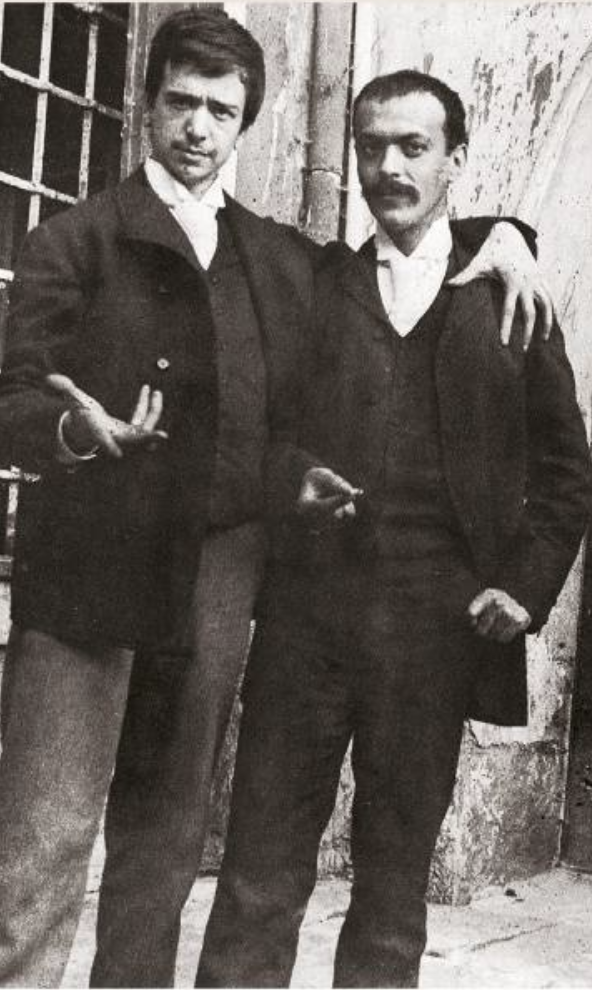
\includegraphics[width=6cm]{veruda}
\end{center}
\caption{Italo Svevo insieme a Umberto Veruda (a sinistra), pittore e amico fraterno, 1890}
\end{figure}

Ad un certo punto il protagonista sente la necessità di vivere la vita, perché quella che lui vive è una sorta di malattia.
Entra in gioco la seconda protagonista femminile, Angiolina, che rappresenta la vita e la salute.
Il protagonista è attratto da questa vita, ma succede che anche il suo rapporto con la donna è fallimentare, perché Angelina non è un personaggio positivo in toto: è giovane, opportunista, ha altri amanti, e il protagonista si innamora di lei, e siccome la donna non corrisponde nella realtà alla fanciulla che ama, ne costruisce un'altra ideale, completamente differente da Angiolina: si costruisce una sorta di donna angelica strutturata secondo il motivo della lirica antica.

Emilio è un inetto che cerca tutta una serie di scusanti, autoinganni, rispetto al suo modo di agire, e anche qui abbiamo un narratore esterno che svela al lettore tutti questi autoinganni del protagonista. Il protagonista mente, e non si capisce se lo fa apposta o se è un modo di autodifendersi e di trovare delle scusanti.

Il narratore è esterno, e la focalizzazione per la maggior parte è quella del protagonista, però a volte il narratore fa come il narratore di \textit{Una Vita}, mettendo a nudo gli autoinganni del protagonista. Non sempre lo fa, e a volte non succede che il narratore intervenga, però il lettore riesce lo stesso a capire che la posizione dell'autore è di distanza rispetto al protagonista: abbiamo l'\textbf{ironia oggettiva} o \textbf{implicita}: il narratore non dice niente, ma il protagonista è smentito dai fatti.
La verità viene svelata dal linguaggio utilizzato dal protagonista, stereotipato, che gli fa perdere credibilità.

\section{T: \textit{Il ritratto dell'inetto}}

In questo brano si evincono quali sono le funzioni e le intenzioni del narratore: è esterno, parla in terza persona. La focalizzazione è quasi sempre quella del protagonista, ma il narratore interviene a chiarire e a smascherare gli autoinganni del protagonista. Ora il narratore interviene con termini che vanno in qualche modo a limitare l'idea di carriera.

Il narratore è onnisciente, cin quanto interviene senza correggere quello che ha detto il protagonista. Il narratore interviene sul non detto, ironizzando sul fatto che la famiglia sia una sorella \textit{non ingombrante}.

Narratore e protagonista fino ad ora hanno parlato di carriera.
Emerge dalla pagina iniziale in senso della “senilità”: Emilio ha paura di affrontare la vita che gli appare piena di pericoli e perciò rinuncia a vivere. Emilio si crea quindi una maschera superomistica, non ha la lucidità di vedersi nella sua effettiva mediocrità di romanziere fallito e sterile.

L’idea di Emilio (inetto) è che questa fase piuttosto grigia sia solamente un periodo di preparazione quando in realtà non è così.
Della psicoanalisi Svevo rifiuta l’aspetto medico e accetta tutti quegli strumenti di analisi che gli sono utili per descrivere i suoi personaggi. Angiolina non è un inetto, è una ragazza povera ma non così tanto da dover soffrire la fame. La salute caratterizza il personaggio di Angelina che non è inetto. A fare contrappeso alla figura dell’inetto abbiamo sempre una figura “illuminata”.

La narrazione è \textbf{eterodiegetica} ma il narratore non si eclissa. Il narratore rappresenta l’alternativa di una prospettiva superiore, più lucida e consapevole e si pone come proposito quello di smascherare impietosamente i suoi autoinganni.
Angelina è la possibilità intravista dal protagonista di creare un diversivo nella sua vita. Il protagonista non parla di carriera, ma di un impieguccio in banca, o di una carriera letteraria.
Questo ci riporta alla distinzione che abbiamo fatto tra Darwin e Shopenhauer, quando nella gita in barca di Alfonso si è parlato della differenza tra colui che vive la vita da spettatore e al lottatore, che invece si fa largo nella vita, questo \textbf{per natura}.
L’idea invece di Emilio, che è inetto, è che questa fase piuttosto grigia sia solo un periodo di preparazione, ma non è così, infatti anche questo personaggio finirà male.
Qui ci sta un  confronto con l’inetto della coscienza di Zeno, è un uomo che ha successo nella vita, è possibile che svevo abbia rivalutato la figura dell’inetto?  Oppure che ne abbia colto qualcosa di positivo?

La salute caratterizza il personaggio che non è inetto, a fare da contrappeso alla figura dell’inetto in ogni romanzo c’è sempre una figura “illuminata”, nella coscienza di Zeno è la moglie.

Quando finalmente Emilio riesce a conquistarla e possederla, non gli piace cosa vede, ha anti amanti, un’arrivista, da lui scaturisce una gelosia che avrà conseguenze nel suo comportamento. Lui quindi ne crea un’altra, più confacente alle sue aspettative, fedele, rappresentazione della donna angelo.

\setcounter{mar}{0}
\begin{quotation}
Subito, con le prime parole che le rivolse, volle avvisarla che non intendeva compromettersi in una relazione troppo seria. Parlò cioé a un dipresso così: - T’amo molto e per il tuo bene desidero ci si metta d’accordo di andare molto cauti. - La parola era tanto prudente ch’era difficile di crederla detta per amore altrui, e un po’ più franca avrebbe dovuto suonare così: - Mi piaci molto, ma nella mia vita non potrai essere giammai più importante di un giocattolo. Ho altri doveri io, la mia carriera, la mia famiglia.

La sua famiglia? Una sola sorella non ingombrante né fisicamente né moralmente, piccola e pallida, di qualche anno più giovane di lui, ma più vecchia per carattere o forse per destino. Dei due, era lui l’egoista, il giovane; ella viveva per lui come una madre dimentica di se stessa, ma ciò non impediva a lui di parlarne come di un altro destino importante legato al suo e che pesava sul suo, e così, sentendosi le spalle gravate di tanta responsabilità, egli traversava la vita cauto, lasciando da parte tutti i pericoli ma anche il godimento, la felicità. A trentacinque anni si ritrovava nell’anima la brama insoddisfatta di piaceri e di amore, e già l’amarezza di non averne goduto, e nel cervello una grande paura di se stesso e della debolezza del proprio carattere, invero piuttosto sospettata che saputa per esperienza.

La carriera di Emilio Brentani era più complicata perché intanto si componeva di due occupazioni e due scopi ben distinti. Da un impieguccio di poca importanza presso una società di assicurazioni, egli traeva giusto il denaro di cui la famigliuola abbisognava. L’altra carriera era letteraria e, all’infuori di una riputazioncella, - soddisfazione di vanità più che d’ambizione - non gli rendeva nulla, ma lo affaticava ancor meno. Da molti anni, dopo di aver pubblicato un romanzo lodatissimo dalla stampa cittadina, egli non aveva fatto nulla, per inerzia non per sfiducia. Il romanzo, stampato su carta cattiva, era ingiallito nei magazzini del libraio, ma mentre alla sua pubblicazione Emilio era stato detto soltanto una grande speranza per l’avvenire, ora veniva considerato come una specie di rispettabilità letteraria che contava nel piccolo bilancio artistico della città. La prima sentenza non era stata riformata, s’era evoluta.

Per la chiarissima coscienza ch’egli aveva della nullità della propria opera, egli non si gloriava del passato, però, come nella vita così anche nell’arte, egli credeva di trovarsi ancora sempre nel periodo di preparazione, riguardandosi nel suo più segreto interno come una potente macchina geniale in costruzione, non ancora in attività. Viveva sempre in un’aspettativa non paziente, di qualche cosa che doveva venirgli dal cervello, l’arte, di qualche cosa che doveva venirgli di fuori, la fortuna, il successo, come se l’età delle belle energie per lui non fosse tramontata.

Angiolina, una bionda dagli occhi azzurri grandi, alta e forte, ma snella e flessuosa, il volto illuminato dalla vita, un color giallo di ambra soffuso di rosa da una bella salute\mat{Descrive il personaggio femminile, ragazza povera ma non troppo, si chiama Angiolina}, camminava accanto a lui, la testa china da un lato come piegata dal peso del tanto oro che la fasciava, guardando il suolo ch’ella ad ogni passo toccava con l’elegante ombrellino come se avesse voluto farne scaturire un commento alle parole che udiva. Quando credette di aver compreso disse: - Strano - timidamente guardandolo sottecchi. - Nessuno mi ha mai parlato così. - Non aveva compreso e si sentiva lusingata al vederlo assumere un ufficio che a lui non spettava, di allontanare da lei il pericolo. L’affetto ch’egli le offriva ne ebbe l’aspetto di fraternamente dolce.

Fatte quelle premesse, l’altro si sentì tranquillo e ripigliò un tono più adatto alla circostanza. Fece piovere sulla bionda testa le dichiarazioni liriche che nei lunghi anni il suo desiderio aveva maturate e affinate, ma, facendole, egli stesso le sentiva rinnovellare e ringiovanire come se fossero nate in quell’istante, al calore dell’occhio azzurro di Angiolina. Ebbe il sentimento che da tanti anni non aveva provato, di comporre, di trarre dal proprio intimo idee e parole: un sollievo che dava a quel momento della sua vita non lieta, un aspetto strano, indimenticabile, di pausa, di pace. La donna vi entrava! Raggiante di gioventù e bellezza ella doveva illuminarla tutta facendogli dimenticare il triste passato di desiderio e di solitudine e promettendogli la gioia per l’avvenire ch’ella, certo, non avrebbe compromesso.

Egli s’era avvicinato a lei con l’idea di trovare un’avventura facile e breve, di quelle che egli aveva sentito descrivere tanto spesso e che a lui non erano toccate mai o mai degne di essere ricordate. Questa s’era annunziata proprio facile e breve. L’ombrellino era caduto in tempo per fornirgli un pretesto di avvicinarsi ed anzi - sembrava malizia! - impigliatosi nella vita trinata della fanciulla, non se n’era voluto staccare che dopo spinte visibilissime. Ma poi, dinanzi a quel profilo sorprendentemente puro, a quella bella salute - ai rétori corruzione e salute sembrano inconciliabili - aveva allentato il suo slancio, timoroso di sbagliare e infine s’incantò ad ammirare una faccia misteriosa dalle linee precise e dolci, già soddisfatto, già felice.

Ella gli aveva raccontato poco di sé e per quella volta, tutto compreso del proprio sentimento, egli non udì neppure quel poco. Doveva essere povera, molto povera, ma per il momento - lo aveva dichiarato con una certa quale superbia - non aveva bisogno di lavorare per vivere. Ciò rendeva l’avventura anche più gradevole, perché la vicinanza della fame turba là dove ci si vuol divertire. Le indagini di Emilio non furono dunque molto profonde ma egli credette che le sue conclusioni logiche, anche poggiate su tali basi, dovessero bastare a rassicurarlo. Se la fanciulla, come si sarebbe dovuto credere dal suo occhio limpido, era onesta, certo non sarebbe stato lui che si sarebbe esposto al pericolo di depravarla; se invece il profilo e l’occhio mentivano, tanto meglio. C’era da divertirsi in ambedue i casi, da pericolare in nessuno dei due.

Angiolina aveva capito poco delle premesse, ma, visibilmente, non le occorrevano commenti per comprendere il resto; anche le parole più difficili avevano un suono di carattere non ambiguo. I colori della vita risaltarono sulla bella faccia e la mano di forma pura, quantunque grande, non si sottrasse a un bacio castissimo d’Emilio.

Si fermarono a lungo sul terrazzo di S. Andrea e guardarono verso il mare calmo e colorito nella notte stellata, chiara ma senza luna. Nel viale di sotto passò un carro e, nel grande silenzio che li circondava, il rumore delle ruote sul terreno ineguale continuò a giungere fino a loro per lunghissimo tempo. Si divertirono a seguirlo sempre più tenue finché proprio si fuse nel silenzio universale, e furono lieti che per tutt’e due fosse scomparso nello stesso istante. - Le nostre orecchie vanno molto d’accordo, - disse Emilio sorridendo.

Egli aveva detto tutto e non sentiva più alcun bisogno di parlare. Interruppe un lungo silenzio per dire: - Chissà se quest’incontro ci porterà fortuna! - Era sincero. Aveva sentito il bisogno di dubitare della propria felicità ad alta voce.

- Chissà? - replicò essa con un tentativo di rendere nella propria voce la commozione che aveva sentita nella sua. Emilio sorrise di nuovo ma di un sorriso che credette di dover celare. Date le premesse da lui fatte, che razza di fortuna poteva risultare ad Angiolina dall’averlo conosciuto?

Poi si lasciarono. Ella non volle ch’egli l’accompagnasse in città ed egli la seguì a qualche distanza non sapendo ancora staccarsene del tutto. Oh, la gentile figura! Ella camminava con la calma del suo forte organismo, sicura sul selciato coperto da una fanghiglia sdrucciolevole; quanta forza e quanta grazia unite in quelle movenze sicure come quelle di un felino.
\end{quotation}
\vfill
\begin{center}
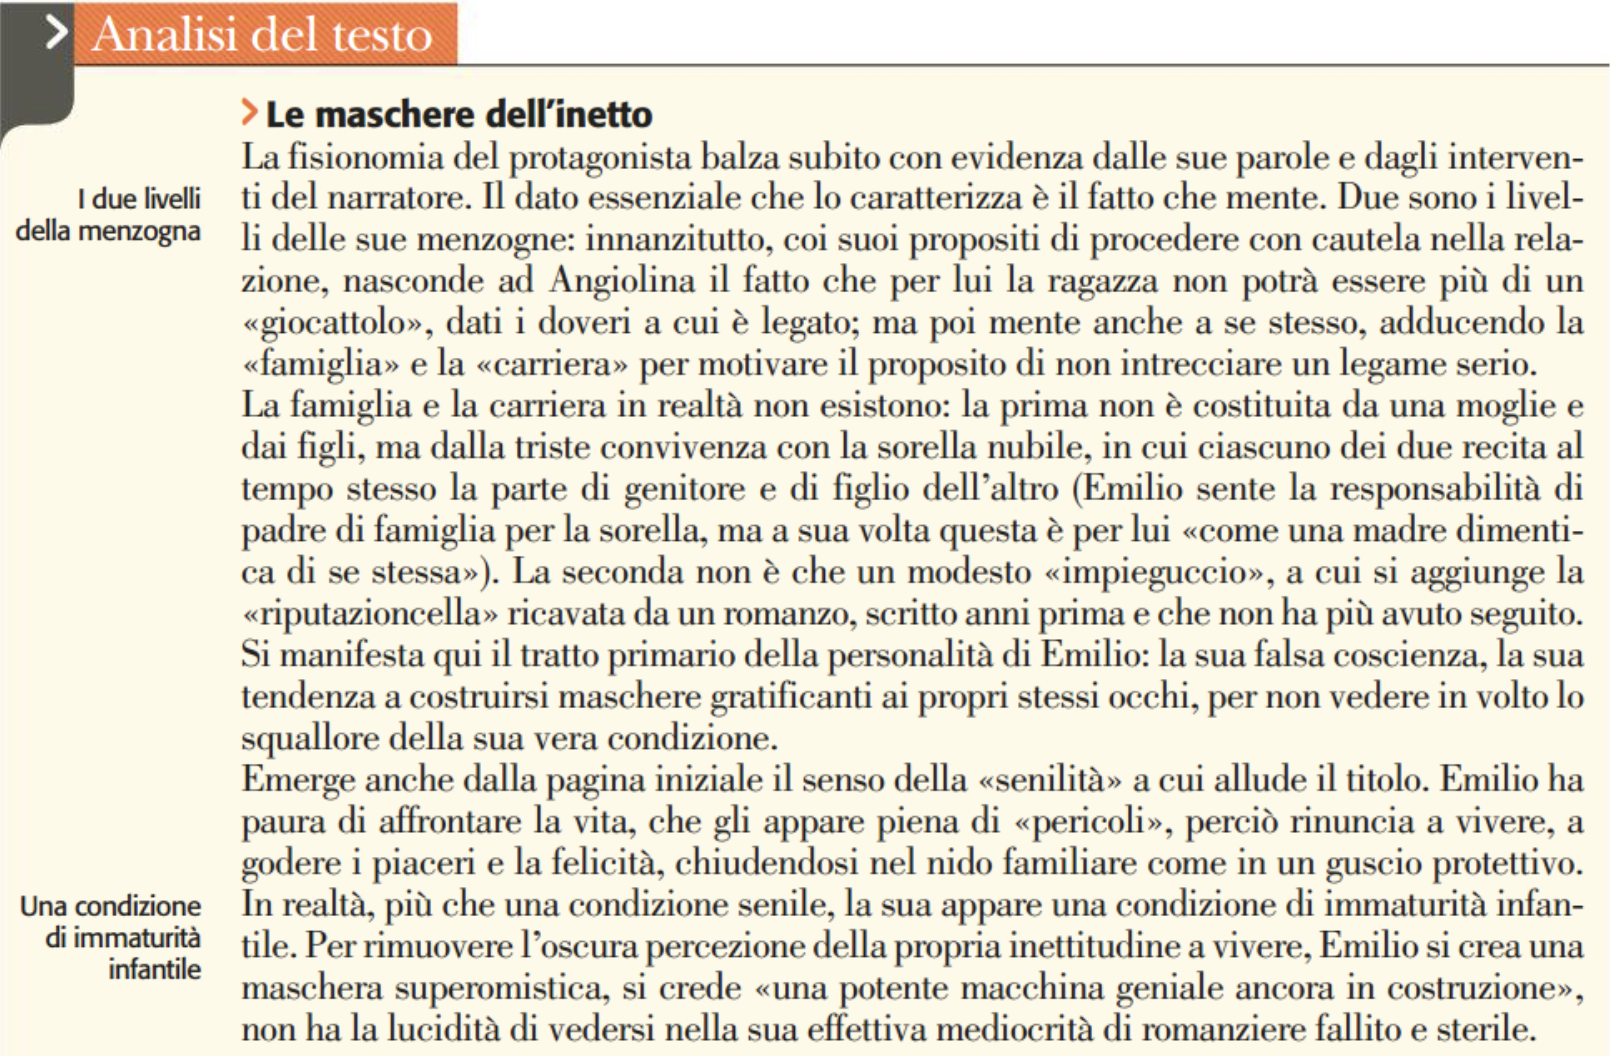
\includegraphics[width=\textwidth]{inetto1}
\end{center}

\begin{center}
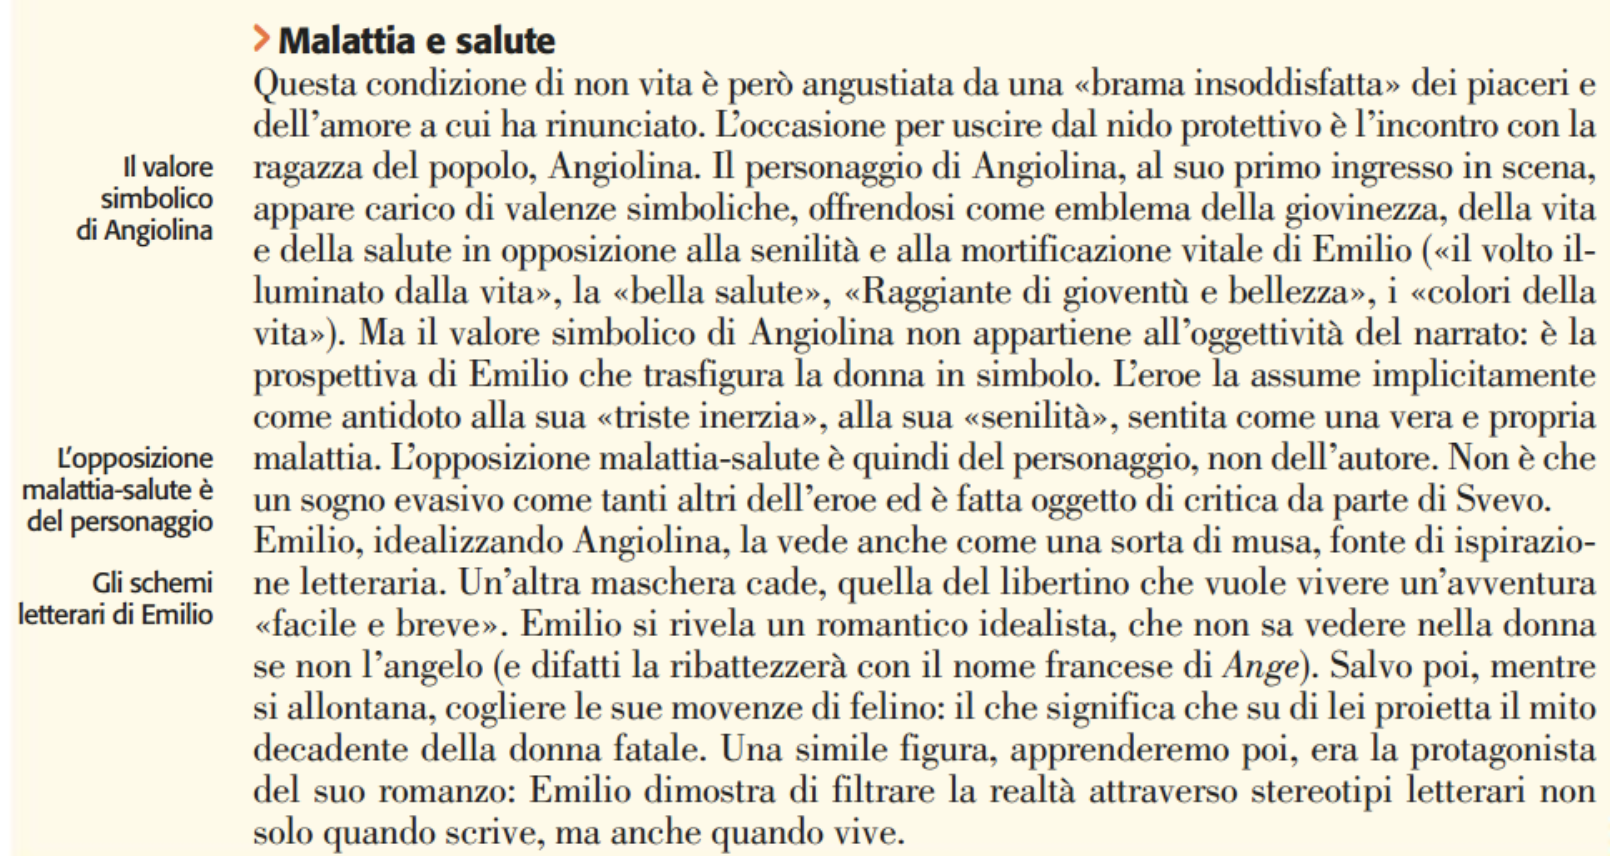
\includegraphics[width=\textwidth]{inetto2}
\end{center}

\begin{center}
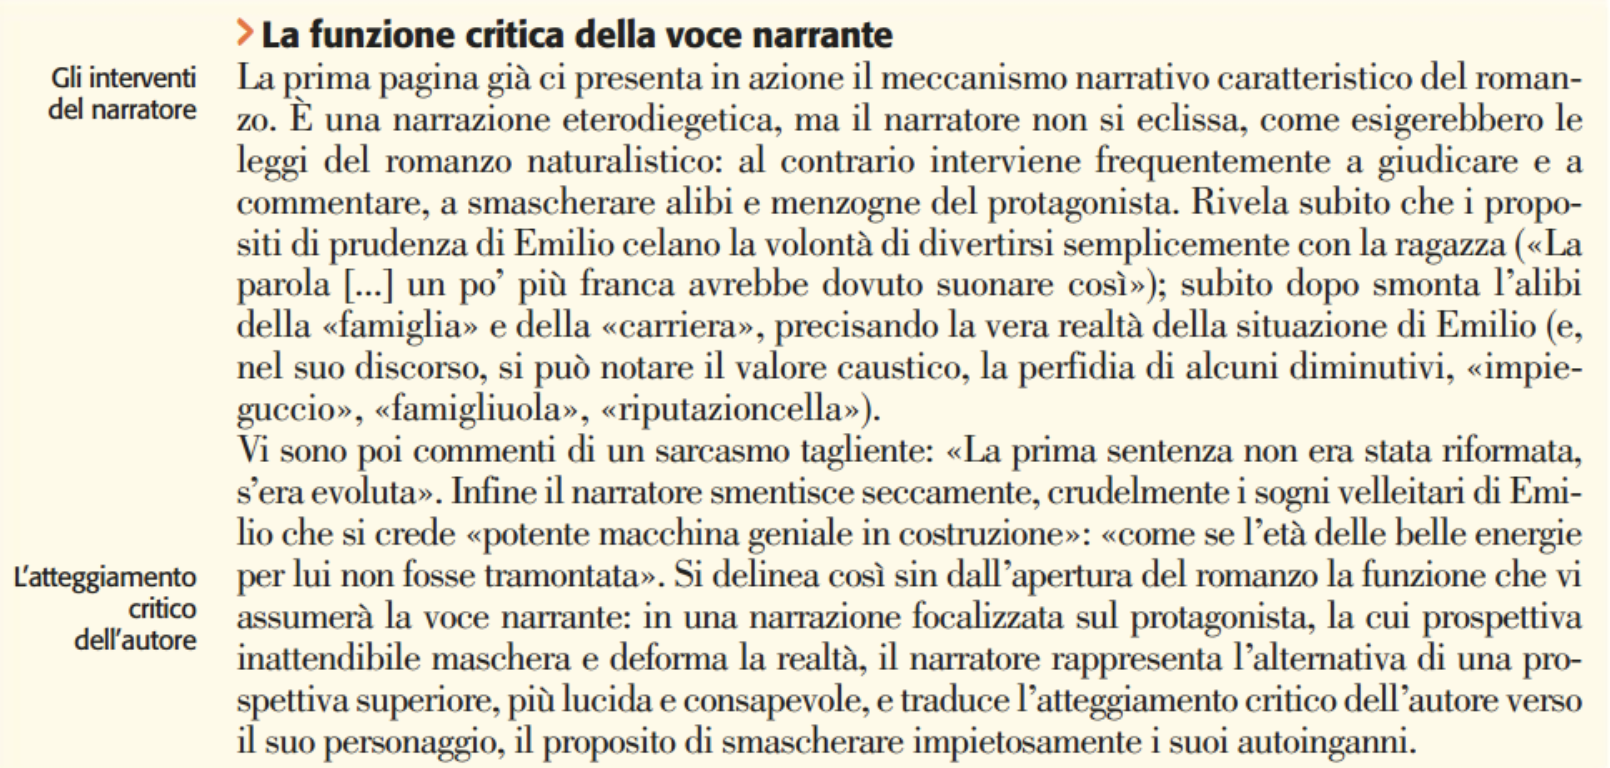
\includegraphics[width=\textwidth]{inetto3}
\end{center}


\chapter{\textit{Coscienza di Zeno}}

Qui a differenza del testo precedente non abbiamo più un narratore interno, è onnisciente perché è il protagonista che parla di se stesso, ma non sa tutto degli altri protagonisti, oltre che essere inattendibile, bugiardo
La malattia di Zeno è il disadattamento, ci sono anche riscontri fisici, la malattia dell’anima diventa malattia fisica. Questo è il filo portante della coscienza di Zeno

È pubblicata nel 1923, e moltissimi anni lo separano dall'ultimo libro pubblicato.
La prospettiva dell'autore cambia, in quanto è passata una guerra mondiale dal precedente...

Questo romanzo probabilmente non avrebbe avuto successo se non fosse che Joyce e Montale ci credettero molto, e gli garantirono un certo successo, nonostante qualche resistenza in Italia: infatti, in Italia alcuni considerano strana e brutta la lingua di Svevo. Alcuni esempi sono
\citazione{"Ero riuscito di fare accettare"\\
"Cosa ha da fare"}

\section{Giacomo Debenedetti: \textit{Una scrittura che morde le cose}}
Si è molto parlato, a proposito di Svevo, del suo presunto "scrivere male". Svevo scrive male se si assume come modello la scrittura di D'Annunzio o comunque la scrittura letteraria della nostra più alta tradizione classicista (da Alfieri a Foscolo a Leopardi). Ma non scrive male se si guarda alla funzionalità delle idee che intende comunicare. Il linguaggio sveviano è uno strumento che, per quanto inelegante, funziona in modo efficace. È questa la tesi del critio letterario e saggista \textbf{Giacomo Debenedetti} (1901-67).

La scrittura sveviana è bruttissima senza dubbio, quando venga messa a confronto con le inflessioni più naturali e mature, a cui i secoli hanno avvezzato la prosa italiana. Ma che, dopo esserne stati sconcertati, si comincia a sentire pronta, precisa a suo modo e ricca di risorse, per finire forse con l'amarla, come si ama l'accento sia pir vizioso di persona che ci tenga incatenati con la sola consistenza del discorso e il calore della comunicativa. Si prova anzi uno specifico e raro piacere a constatare come l'elocuzione e la sintassi di Svevo, malgrado tutti gli arbitrii e le cacofonie esterne e interne, arrivino ad attaccare e mordere le cose; e come da quelle disuguaglianze e incertezze formali balzi l'evidenza di un ritratto, la netta figura di una situazione o di un movimento. Ed è, direi, il piacere di assistere al funzionamento di un utensile efficace, per quanto inelegante

Probabilmente alcune scelte formali erano estremamente adatte a tratteggiare il personaggio dell'inetto.

\section{T: \textit{Prefazione}}

\begin{quotation}
Io sono il dottore di cui in questa novella si parla talvolta con parole poco lusinghiere. Chi di psico-analisi s’intende, sa dove piazzare l’antipatia che il paziente mi dedica.

Di psico-analisi non parlerò perché qui entro se ne parla già a sufficienza. Debbo scusarmi di aver indotto il mio paziente a scrivere la sua autobiografia; gli studiosi di psico-analisi arricceranno il naso a tanta novità. Ma egli era vecchio ed io sperai che in tale rievocazione il suo passato si rinverdisse, che l’autobiografia fosse un buon preludio alla psico-analisi. Oggi ancora la mia idea mi pare buona perché mi ha dato dei risultati insperati, che sarebbero stati maggiori se il malato sul più bello non si fosse sottratto alla cura truffandomi del frutto della mia lunga paziente analisi di queste memorie.

Le pubblico per vendetta e spero gli dispiaccia. Sappia però ch'io sono pronto di dividere con lui i lauti onorari che ricaverò da questa pubblicazione a patto egli riprenda la cura. Sembrava tanto curioso di se stesso! Se sapesse quante sorprese potrebbero risultargli dal commento delle tante verità e bugie ch'egli ha qui accumulate!...

Dottor S.
\end{quotation}

È il dottor S che parla
Abbiamo parlato di una certa resistenza di Svevo alla psicoanalisi, ma questo non significa che Svevo rifiutasse completamente l'analisi: in alcuni brani Svevo accenna ad un'auto analisi, a cui crede molto: è un sistema "casalingo" di Svevo, e possiamo immaginare che questo romanzo, con forti riferimenti autobiografici, sia una sorta di autoanalisi da parte dell'autore, casalinga, bonaria, e anche un po' ironica.

Quest'opera nasce dal rifiuto di Zeno di continuare la cura del dottor S, che per vendicarsi pubblica tutto ciò che il paziente ha scritto fino a quel momento.
Ci mette in guardia della sua inaffidabilità.

Il motivo del manoscritto ritrovato è un topos letterario utilizzato per introdurre il romanzo. Qui è qualcosa di molto simile.
Se negli altri casi il ritrovamento del manoscritto serviva a dare veridicità alla vicenda, qui succede che il dottor S ci mette in guardia rispetto alle tante bugie dette dall'autore.

Il narratore è interno, che parla in prima persona (è lo stesso Zeno), ed è inattendibile: entrano in gioco gli autoinganni e tutte quelle costruzioni che il protagonista fa per giustificarsi, e noi non abbiamo più nessun parametro per capire se si tratta di verità oppure no. È il relativismo più assoluto.

È come se Svevo ci dicesse che non ci sono più riferimenti oggettivi, ed è la maniera in cui Svevo ci mette di fronte alla fine di quell'atteggiamento di fiducia tipico del positivismo nella ragione e nei dati oggettivi.

Ci sono una serie di elementi estremamente significativi in questo senso: esempio è l'uso del tempo: non c'è un tempo oggettivo, e l'opera non si svolge in senso diacronico, ma abbiamo un tempo misto, ovvero una sovrapposizione di piani temporali che avviene nello stesso brano e nello stesso momento; è un tentativo di riprodurre i momenti veloci della nostra mente, così come lo è il flusso di coscienza: è una tecnica narrativa che serve a riprodurre il lavorio della nostra mente e del nostro inconscio.

Zeno giustifica la sua menzogna nello scrivere
\citazione{Con ogni nostra parola toscana noi mentiamo! Se egli sapesse come raccontiamo con predilezione tutte le cose per le quali abbiamo pronta la frase e come evitiamo quelle che ci obbligherebbero di ricorrere al vocabolario! È proprio così che scegliamo dalla nostra vita gli episodi da notarsi. Si capisce come la nostra vita avrebbe tutt'altro aspetto se fosse detta nel nostro dialetto.}

\section{T: \textit{Il fumo}}

Una novità rispetto al romanzo tradizionale è che non si proceda più attraverso una narrazione diacronica: ci sono delle sovrapposizione temporali, che vengono definite tempo misto;
i capitoli sono raggruppati in ordine tematico, non cronologico; alla fine del romanzo si può ricostruire una sorta di fabula, che non è la cosa più importante.

Forse Zeno non voleva effettivamente guarire, perché il fumo gli serviva a giustificare la sua inettitudine

\subsection*{Righe 1-6}

\begin{quotation}
Il dottore al quale ne parlai mi disse d’iniziare il mio lavoro con un’analisi storica della mia propensione al fumo:

- Scriva! Scriva! Vedrà come arriverà a vedersi intero.

Credo che del fumo posso scrivere qui al mio tavolo senz’andar a sognare su quella poltrona. Non so come cominciare e invoco l’assistenza delle sigarette tutte tanto somiglianti a quella che ho in mano.
\end{quotation}

Qui siamo al presente, ovvero il momento in cui Zeno sta scrivendo. La narrazione inizia con un momento X, che è quello dello Zeno anziano che scrive

\subsection*{Righe 7-9}

\begin{quotation}
Oggi scopro subito qualche cosa che piú non ricordavo. Le prime sigarette ch’io fumai non esistono piú in commercio. Intorno al ’70 se ne avevano in Austria di quelle che venivano vendute in scatoline di cartone munite del marchio dell’aquila bicipite.
\end{quotation}

Se identifichiamo Zeno con Svevo, negli anni '70 Zeno era molto giovane. In ogni caso anche Zeno, da quello che si dice dopo, era giovane a quell'epoca.

Senza nessuna analessi siamo passati al passato. Ciò che rende plausibile questi passaggi è il fatto che egli stia scrivendo in base ai suoi ricordi, in modo naturale, come se affiorassero i ricordi.

Qui abbiamo il passato, che si va a sovrapporre al tempo presente in cui scrive.

\subsection*{Righe 9-13}

\begin{quotation}
Ecco: attorno a una di quelle scatole s’aggruppano subito varie persone con qualche loro tratto, sufficiente per suggerirmene il nome, non bastevole però a commovermi per l’impensato incontro. Tento di ottenere di piú e vado alla poltrona: le persone sbiadiscono e al loro posto si mettono dei buffoni che mi deridono. Ritorno sconfortato al tavolo.
\end{quotation}

Il ricordo nasce intorno alle sigarette, gli riaffiorano alla mente i ricordi dei volti delle persone che lo avevano accompagnato nelle sue prime scorribande.

\subsection*{Righe 14-18}

\begin{quotation}
Una delle figure, dalla voce un po’ roca, era Giuseppe, un giovinetto della stessa mia età, e l’altra, mio fratello, di un anno di me piú giovine e morto tanti anni or sono. Pare che Giuseppe ricevesse molto denaro dal padre suo e ci regalasse di quelle sigarette. Ma sono certo che ne offriva di piú a mio fratello che a me. Donde la necessità in cui mi trovai di procurarmene da me delle altre. Cosí avvenne che rubai. D’estate mio padre abbandonava su una sedia nel tinello il suo panciotto nel cui taschino si trovavano sempre degli spiccioli: mi procuravo i dieci soldi occorrenti per acquistare la preziosa scatoletta e fumavo una dopo l’altra le dieci sigarette che conteneva, per non conservare a lungo il compromettente frutto del furto.
\end{quotation}

L'episodio raccontato dopo è quando ruba le sigarette al padre, che lo scopre: mentirà al padre. Da quel momento non ruberà mai più

\subsection*{Righe 23-25}

\begin{quotation}
Tutto ciò giaceva nella mia coscienza a portata di mano. Risorge solo ora perché non sapevo prima che potesse avere importanza. Ecco che ho registrata l’origine della sozza abitudine e (chissà?) forse ne sono già guarito.
\end{quotation}

Ricordiamo che la psicoanalisi serve a recuperare il rimosso, e in qualche modo mette l'individuo in relazione con la sua malattia e con la capacità di riuscire a darne una spiegazione: nel tentativo di ricordare quando ha iniziato a fumare, Zeno si mette in relazione con la possibilità di spiegare l'origine di quella abitudine.

\subsection*{Righe 45-47}

\begin{quotation}
 La dolcezza che in quell’età s’accompagna al riposo dopo una grande stanchezza, m’è evidente come un’immagine a sé, tanto evidente come se fossi adesso là accanto a quel caro corpo che piú non esiste.
\end{quotation}

È rievocato un episodio, sempre legato al fumo, di quando Zeno, un giorno, ancora bambino, tornato da una gita è sul divano, e fa finta di dormire per sentire cosa dicono i grandi.

Mentre è nel dormiveglia egli sente dal padre che si lamenta con la madre di non trovare più i suoi mozziconi (Zeno glieli rubava). La madre, quando sta per parlare, gli fa cenno di parlare sottovoce, perché Zeno stava dormendo.

Zeno è contento che il padre sia stato redarguito dalla madre in rispetto di lui che sta dormendo

\subsection*{Righe 70-77}

\begin{quotation}
Io apersi a mezzo gli occhi e guardai mia madre. Essa s’era rimessa al suo lavoro, ma continuava a sorridere. Certo non pensava che mio padre stesse per ammattire per sorridere cosí delle sue paure. Quel sorriso mi rimase tanto impresso che lo ricordai subito ritrovandolo un giorno sulle labbra di mia moglie.
\end{quotation}

Non è una prolessi, ma abbiamo il futuro che si stende naturalmente così, sul passato e sul presente.

\begin{center}
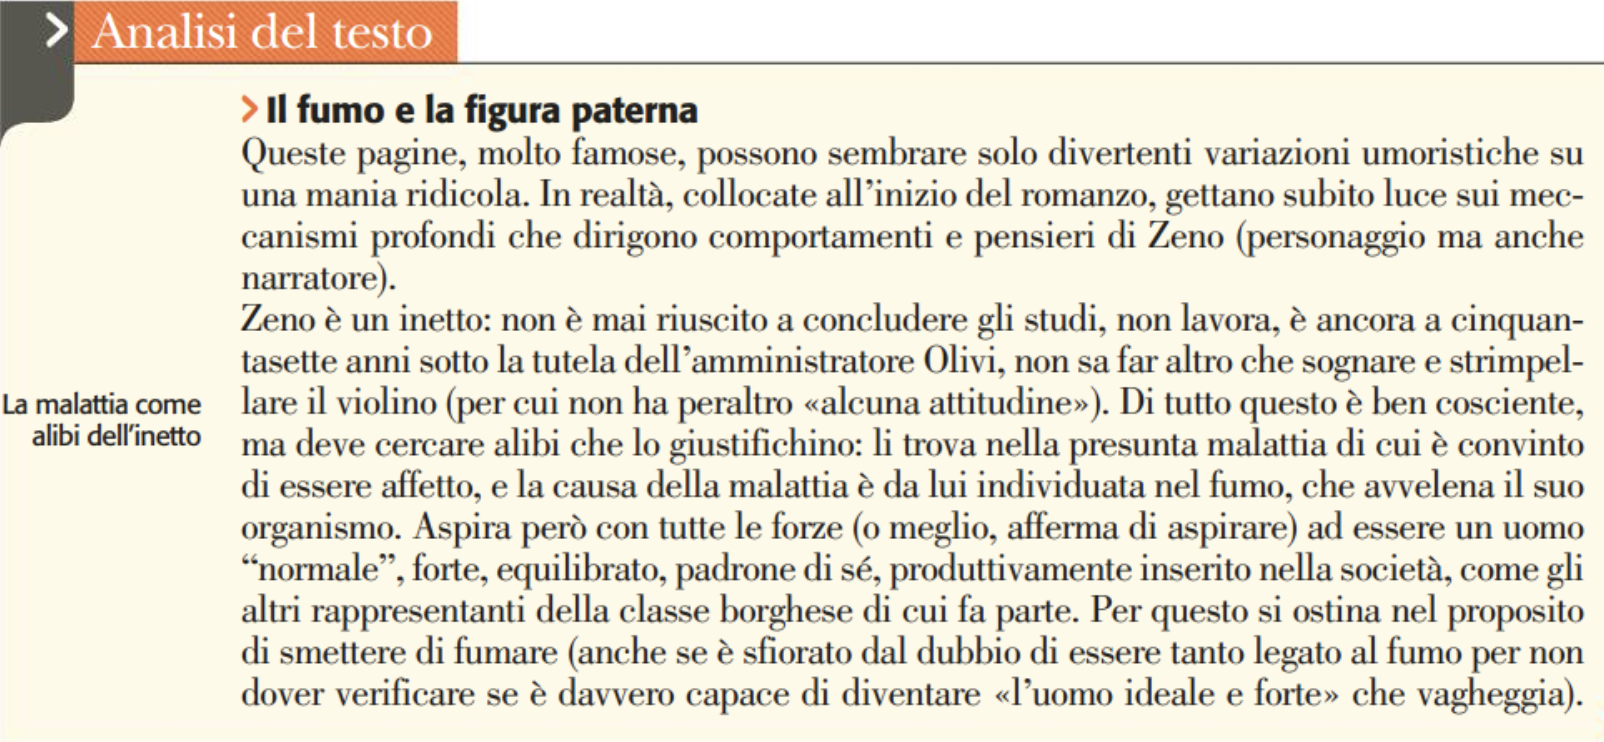
\includegraphics[width=\textwidth]{fumo1}
\end{center}

\begin{center}
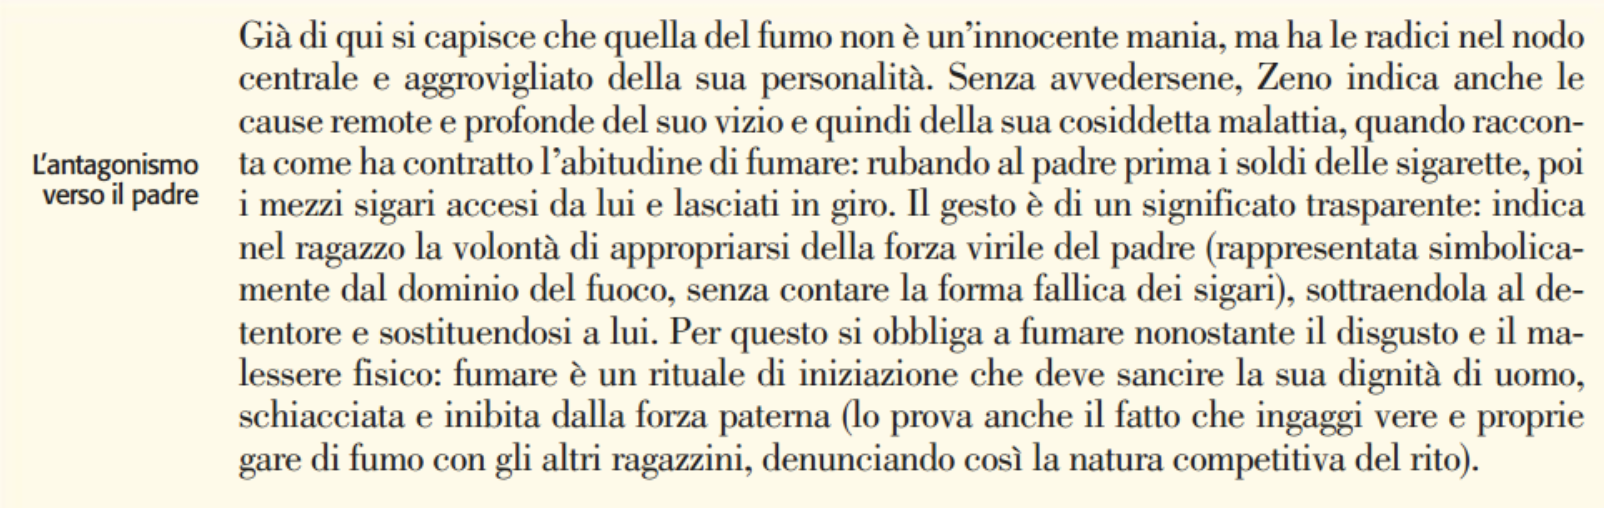
\includegraphics[width=\textwidth]{fumo2}
\end{center}
\vfill
\begin{center}
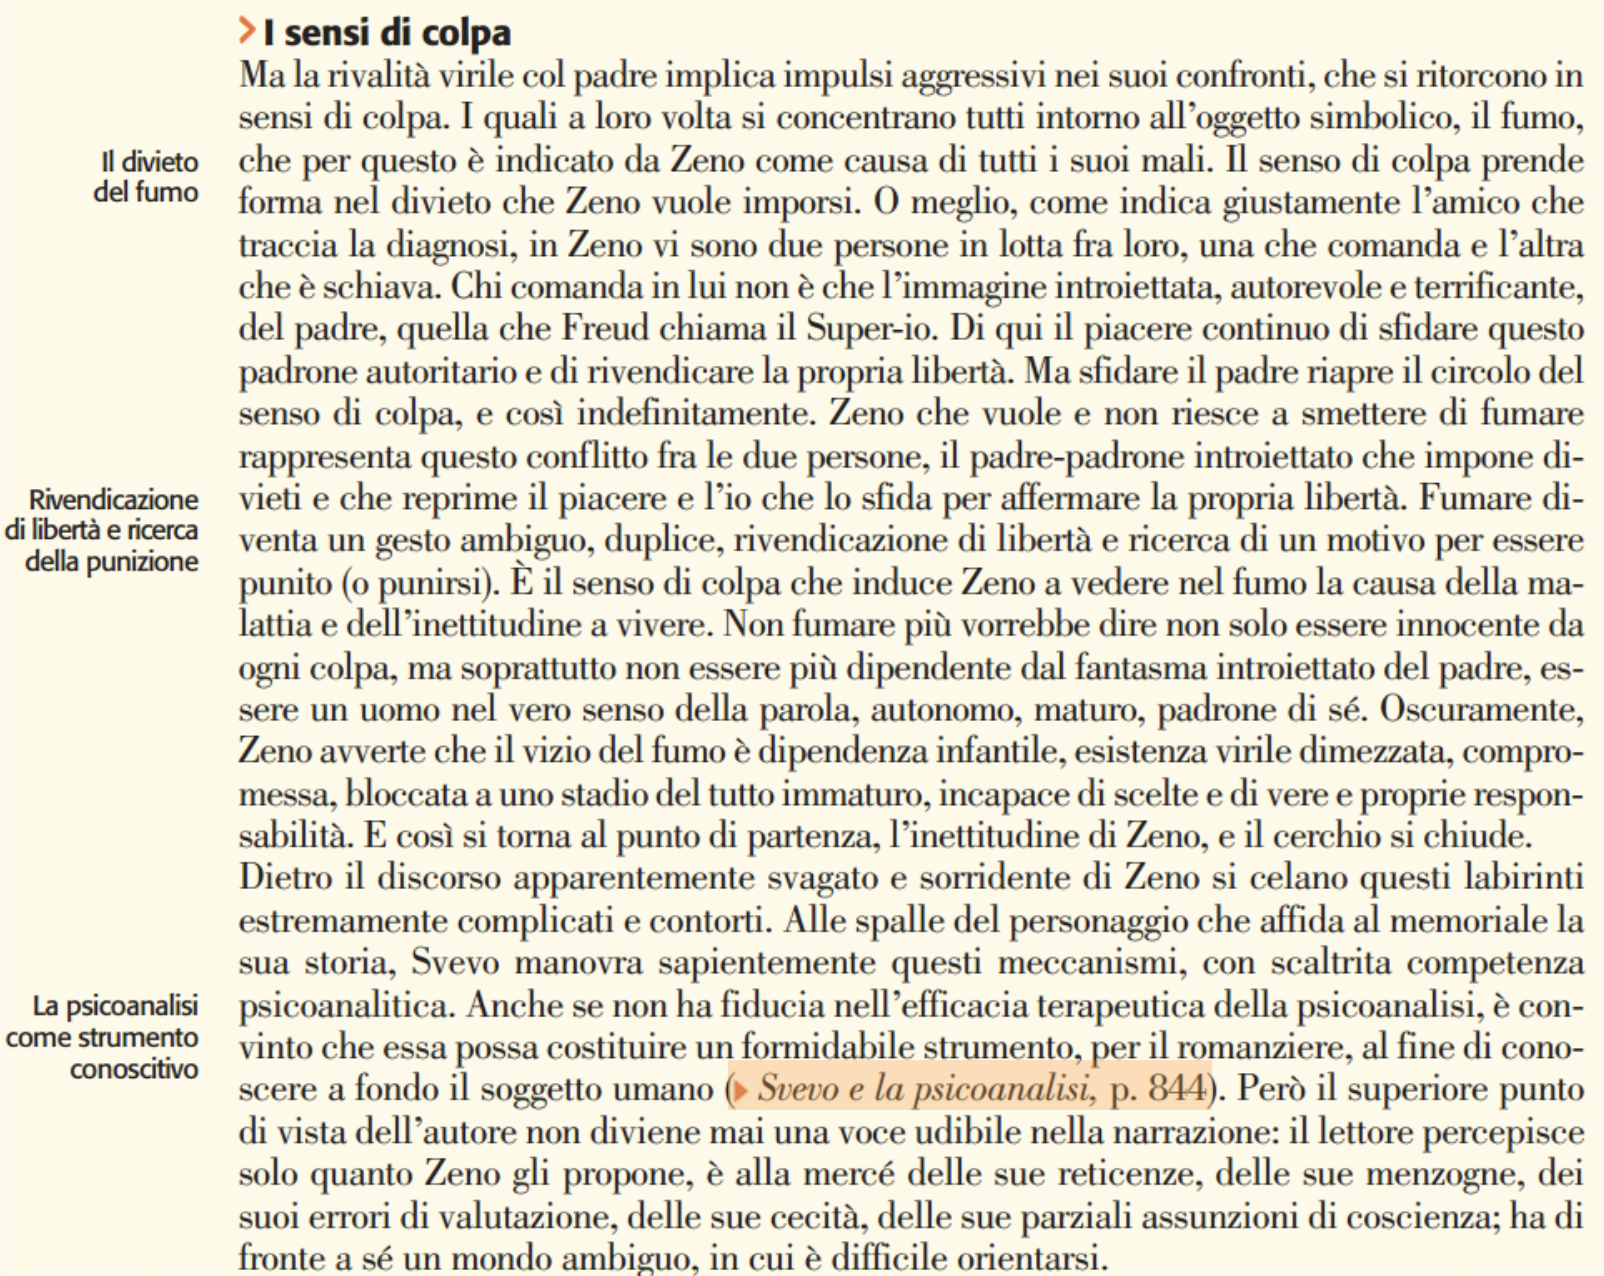
\includegraphics[width=\textwidth]{fumo3}
\end{center}

\section{T: \textit{La morte del padre}}

Siamo portati a pensare che Zeno menta, soprattutto riguardo all'affetto che cerca di dimostrare nei confronti del padre.

Zeno sta raccontando gli ultimi giorni di vita del padre, e poi l'ultimo gesto. Il padre tenta di alzarsi, Zeno lo spinge giù nel letto: il padre prima di morire ha le braccia sollevate, e mentre muore la mano gli ricade sul volto di Zeno, come uno schiaffo.

Quello potrebbe benissimo non essere uno schiaffo, ma Zeno non ne è sicuro: ha dei sensi di colpa nei confronti del padre, e ha paura che l'ultimo gesto del padre sia stato per punirlo.

\subsection*{Riga 19-21}

\begin{quotation}
Sono in complesso cose recenti e per ricordare il mio enorme dolore e ogni particolare della sventura non ho certo bisogno di sognare come vogliono i signori dell’analisi.
\end{quotation}

Frecciatina ai signori dell'analisi.

\subsection*{Righe 71-76}

\begin{quotation}
Per lui il cuore non pulsava e non v’era bisogno di ricordare valvole e vene e ricambio per spiegare come il suo organismo viveva. Niente movimento perché l’esperienza diceva che quanto si moveva finiva coll’arrestarsi. Anche la terra era per lui immobile e solidamente piantata su dei cardini. Naturalmente non lo disse mai, ma soffriva se gli si diceva qualche cosa che a tale concezione non si conformasse. M’interruppe con disgusto un giorno che gli parlai degli antipodi. Il pensiero di quella gente con la testa all’ingiú gli sconvolgeva lo stomaco.
\end{quotation}

Anche la sera in cui la prima volta il padre si ammala, i due avevano avuto una discussione a tavola, sulla forma della terra. Il padre rappresenta quell'ideale borghese, anche magari limitato (ha le sue certezze e non accetta altre verità). Il padre sostiene che la terra è immobile, mentre Zeno vuole fargli notare che non è così.

Vediamo un perfetto borghese, l'antagonista dell'inetto, che viene descritto in termini non completamente positivi: è come se Zeno, inetto, nel tentativo di spiegare il modo di comportarsi degli altri, nell'incapacità di spiegare le loro ragioni, ne mettesse in luce i limiti.

Succede anche per la descrizione di Augusta, la moglie. È brutta, ma molto sana e molto borghese. Mentre la descrive lui mette in luce alcuni aspetti, che a sua opinione sono molto positivi, ma che in realtà non lo sono tanto: "ignorava che quando a questo mondo ci si univa, l'unione sarebbe durata poco". Alla fine Zeno dice che, analizzando la sua salute, la trasforma in malattia, ma che egli crede nonostante questo che egli sia molto sana. (\emph{p. 822-823})

Possiamo quindi vedere che in quest'ultimo romanzo l'inetto è meno negativo come personaggio

Questo inetto cos'ha in più rispetto agli inetti precedenti e rispetto ai sani? Ha consapevolezza del suo essere incompleto: i sani e i forti hanno coscienza della loro forza e della loro salute, e hanno la coscienza dell'essere perfetti, e quindi non sono aperti al cambiamento.
L'inetto, invece, sa di essere imperfetto, e quindi è più aperto al miglioramento. Questo è uno spiraglio positivo nella valutazione dell'inetto.

\subsection*{Righe 218-242}

\begin{quotation}
Fu allora che avvenne la scena terribile che non dimenticherò mai e che gettò lontano lontano la sua ombra, che offuscò ogni mio coraggio, ogni mia gioia. Per dimenticarne il dolore, fu d’uopo che ogni mio sentimento fosse affievolito dagli anni.

L’infermiere mi disse:

- Come sarebbe bene se riuscissimo di tenerlo a letto. Il dottore vi dà tanta importanza!

Fino a quel momento io ero rimasto adagiato sul sofà. Mi levai e andai al letto ove, in quel momento, ansante piú che mai, l’ammalato s’era coricato. Ero deciso: avrei costretto mio padre di restare almeno per mezz’ora nel riposo voluto dal medico. Non era questo il mio dovere?

Subito mio padre tentò di ribaltarsi verso la sponda del letto per sottrarsi alla mia pressione e levarsi. Con mano vigorosa poggiata sulla sua spalla, gliel’impedii mentre a voce alta e imperiosa gli comandavo di non moversi. Per un breve istante, terrorizzato, egli obbedí. Poi esclamò:

- Muoio!

E si rizzò. A mia volta, subito spaventato dal suo grido, rallentai la pressione della mia mano. Perciò egli poté sedere sulla sponda del letto proprio di faccia a me. Io penso che allora la sua ira fu aumentata al trovarsi - sebbene per un momento solo - impedito nei movimenti e gli parve certo ch’io gli togliessi anche l’aria di cui aveva tanto bisogno, come gli toglievo la luce stando in piedi contro di lui seduto. Con uno sforzo supremo arrivò a mettersi in piedi, alzò la mano alto alto, come se avesse saputo ch’egli non poteva comunicarle altra forza che quella del suo peso e la lasciò cadere sulla mia guancia. Poi scivolò sul letto e di là sul pavimento. Morto!

Non lo sapevo morto, ma mi si contrasse il cuore dal dolore della punizione ch’egli, moribondo, aveva voluto darmi. Con l’aiuto di Carlo lo sollevai e lo riposi in letto. Piangendo, proprio come un bambino punito, gli gridai nell’orecchio:

- Non è colpa mia! Fu quel maledetto dottore che voleva obbligarti di star sdraiato!

Era una bugia. Poi, ancora come un bambino, aggiunsi la promessa di non farlo piú:

- Ti lascerò movere come vorrai.

L’infermiere disse:

- È morto.

Dovettero allontanarmi a viva forza da quella stanza. Egli era morto ed io non potevo piú provargli la mia innocenza!
\end{quotation}

In una prima analisi quello è uno schiaffi, e lui non ha neanche capito che il padre è morto.

\begin{center}
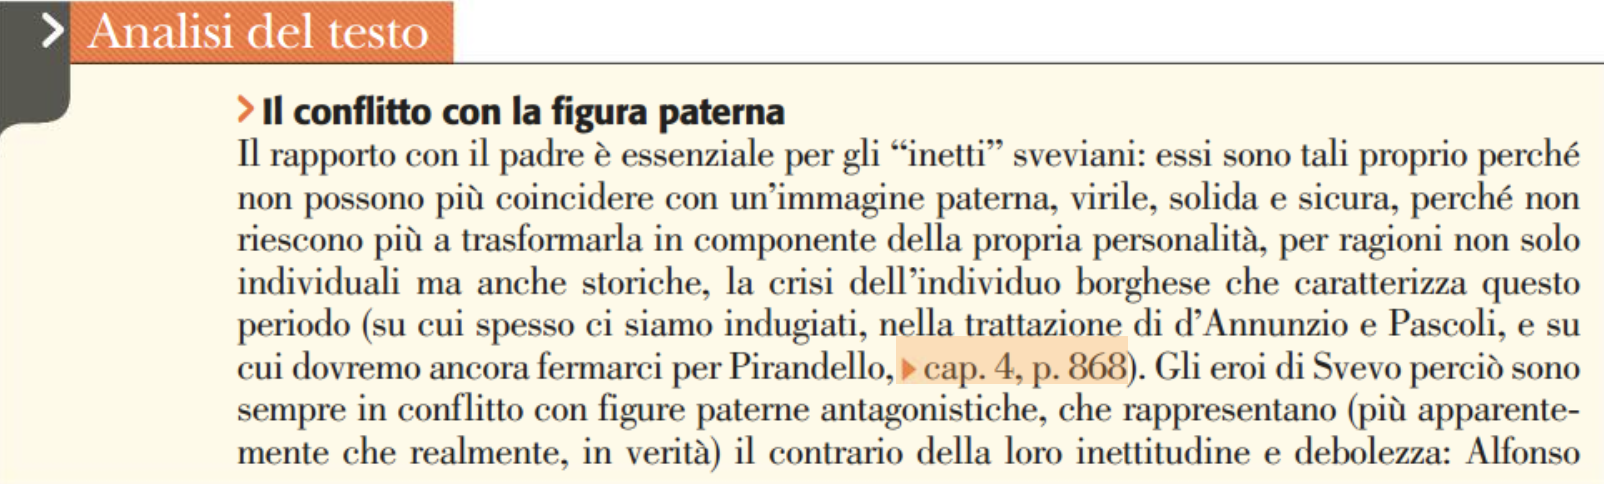
\includegraphics[width=\textwidth]{padre1}
\end{center}
\vfill
\begin{center}
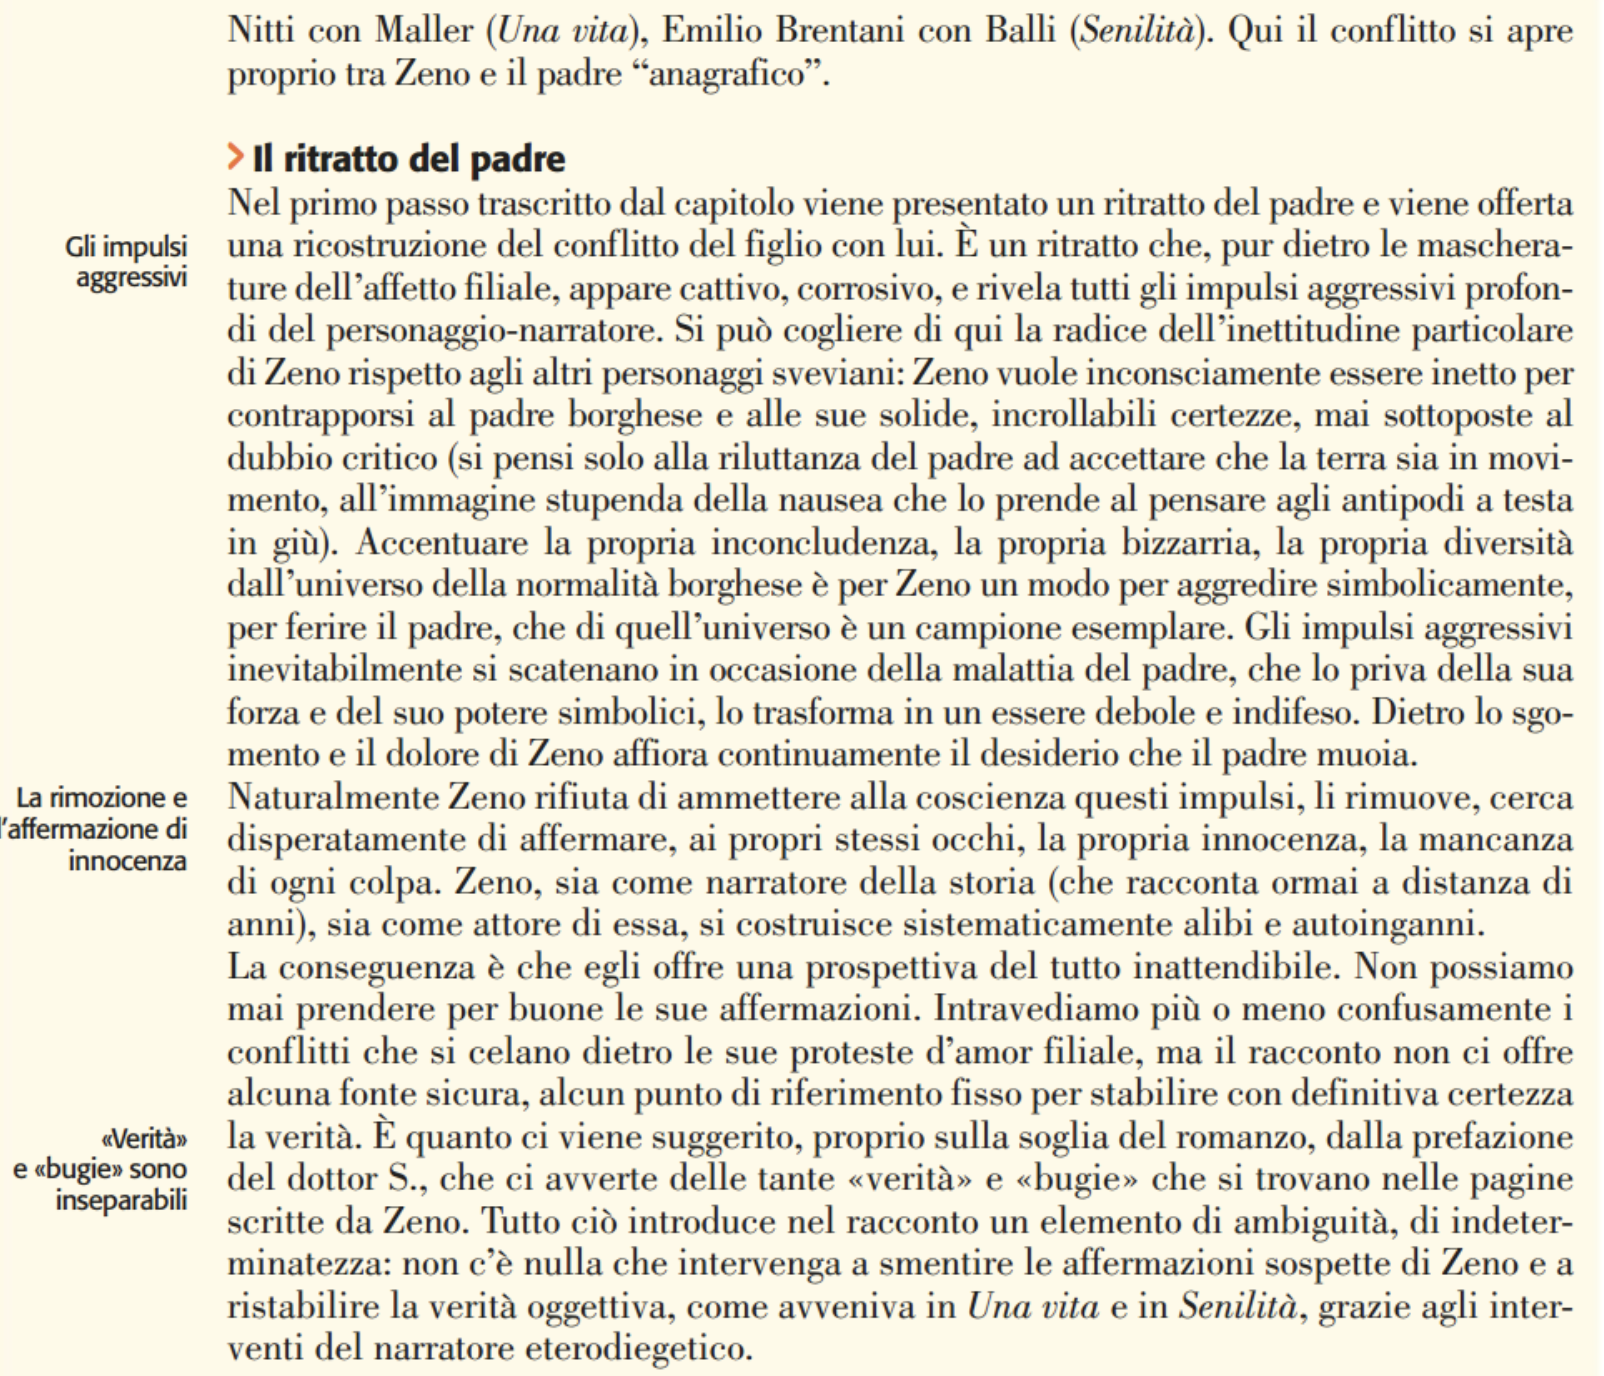
\includegraphics[width=\textwidth]{padre2}
\end{center}
\vfill
\begin{center}
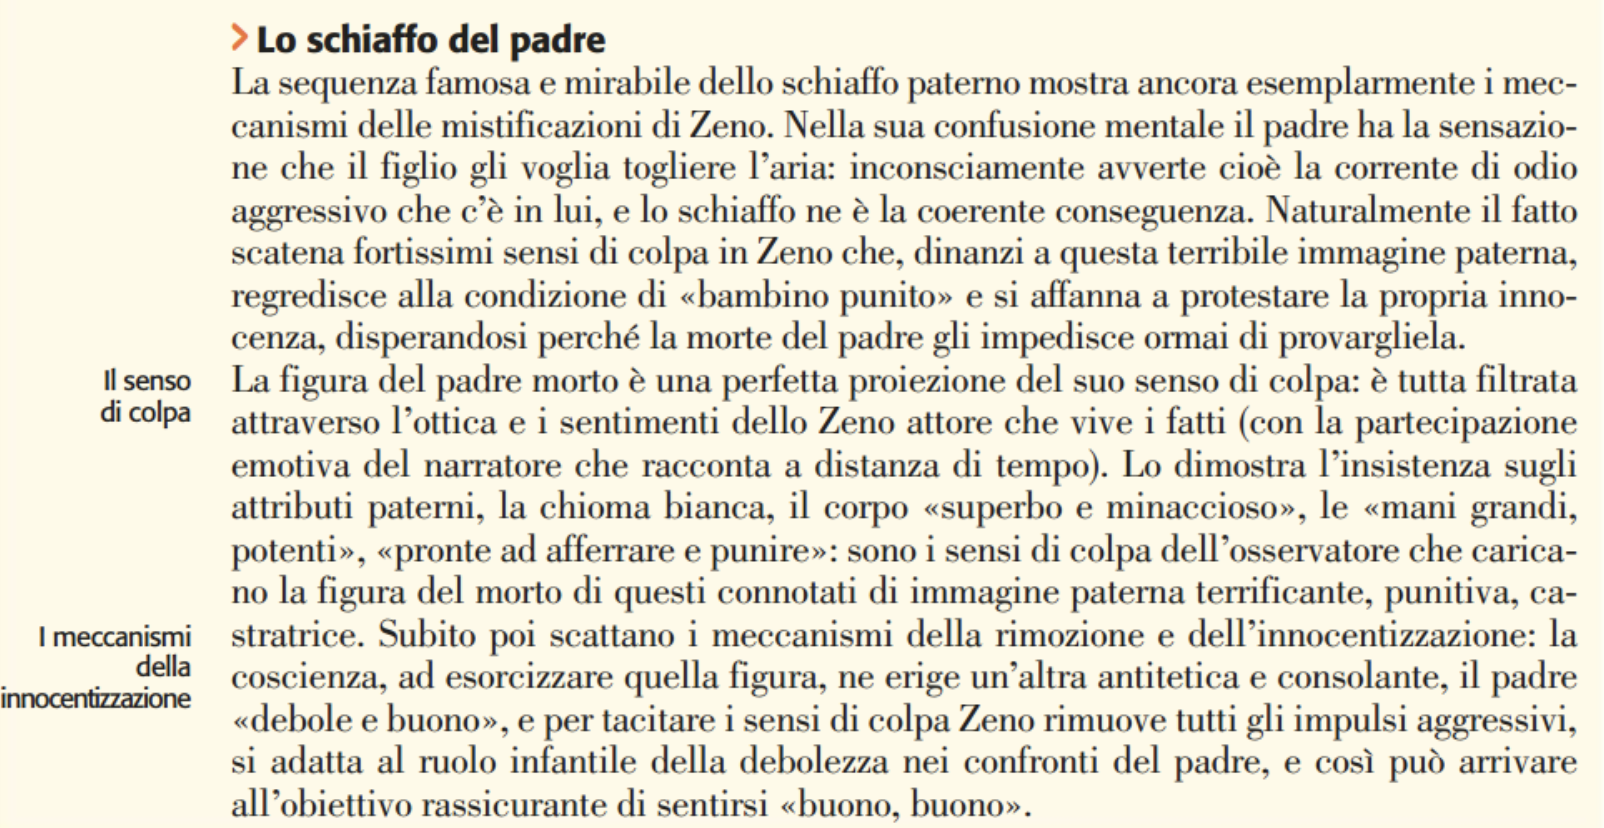
\includegraphics[width=\textwidth]{padre3}
\end{center}
\vfill
\newpage
\section{T: \textit{La profezia di un'apocalisse cosmica}}

\subsection*{Righe 11-21}

\begin{quotation}
Qualunque sforzo di darci la salute è vano. Questa non può appartenere che alla bestia che conosce un solo progresso, quello del proprio organismo. Allorché la rondinella comprese che per essa non c’era altra possibile vita fuori dell’emigrazione, essa ingrossò il muscolo che muove le sue ali e che divenne la parte piú considerevole del suo organismo. La talpa s’interrò e tutto il suo corpo si conformò al suo bisogno. Il cavallo s’ingrandí e trasformò il suo piede. Di alcuni animali non sappiamo il progresso, ma ci sarà stato e non avrà mai leso la loro salute. 
\end{quotation}

Zeno esprime la teoria secondo cui l'uomo sfugge alla selezione naturale di Darwin.

L'uomo è il soggetto principale del progresso, ma non quello fisico: Zeno vuole dire che il progresso dell'uomo non è dovuto a qualche miglioramento del suo organismo, ma per qualche ordigno

\subsection*{Righe 29-31}

\begin{quotation}
Quando i gas velenosi non basteranno piú, un uomo fatto come tutti gli altri, nel segreto di una stanza di questo mondo, inventerà un esplosivo incomparabile, in confronto al quale gli esplosivi attualmente esistenti saranno considerati quali innocui giocattoli.
\end{quotation}

Una visione apocalittica, il cui senso preciso ci sfugge. Il brano è scritto dopo la prima guerra mondiale, che può aver avuto la sua influenza.

\part{Pirandello}

\chapter{Introduzione e caratteri generali}

Con Pirandello vediamo la fine delle certezze tipiche della realtà disegnata dal pensiero positivista.
Un ulteriore e definitivo passo avanti: la realtà oggettiva non esiste ed è anche impossibile descriverla ed evocarla attraverso la letteratura: non esistono uomini eccezionali, non esiste il superuomo, e non esiste alcun poeta o veggente in grado di cogliere quelle corrispondenze di cui parlano tanti poeti decadenti (e anche Pascoli).

Arte e letteratura saranno molto particolari: troveranno il loro compimento soprattutto con il teatro con Pirandello. Le prime rappresentazioni teatrali finirono con il pubblico che usciva inviperito, con un clamoroso insuccesso.

Non c'è più alcuna realtà oggettiva, né da vivere né da descrivere.

\section{Biografia}

Pirandello nasce nel 1867, in Sicilia come Verga, tanto che alcuni racconti giovanili sono stati paragonati alle novelle di Verga.
Nasce a Girgenti, da un padre proprietario di una miniera di zolfo (condizione piuttosto agiata).

Compie gli studi prima a Palermo, e poi a Roma. Studia lettere.
Per degli screzi finisce il suo percorso di studi a Bon, in Germania, dove si laurea con una tesi in filologia sul dialetto di Girgenti.

Inizia la sua produzione nel 1901: esce il primo romanzo, \textit{L'esclusa}. Era stato messo in quartiere alla fine dell'Ottocento

Pirandello è uno dei pochi che ha toccato tutti i generi letterari, dalla poesia, al romanzo, al dramma, al saggio. Si occupa anche di cinema: quando è morto si stava occupando della realizzazione cinematografica de \textit{Il fu Mattia Pascal}.

Nel 1903 c'è un avvenimento parecchio destabilizzante nella vita di Pirandello: la miniera del padre viene distrutta, e Pirandello subisce il declassamento: conosce la povertà. Nel frattempo si era sposato, e i soldi della dote della moglie erano stati investiti in queste miniere.
La moglie, che aveva una personalità particolare, ebbe un peggioramento incredibile nelle sue crisi nervose.

Nel 1904 esce \textit{Il fu Mattia Pascal}. Pirandello scrive il suo romanzo nel periodo in cui si acutizza la malattia nervosa della moglie: il tema della pazzia acquisisce un ruolo preponderante nella sua narrazione.
Sebbene non abbia approfondito l'opera di Freud, sicuramente aver assistito la moglie ha influito moltissimo sulle tematiche affrontate da Pirandello. Molti suoi personaggi finiscono pazzi e ricoverati in cliniche e ospizi: è quasi il tema base.

Nel 1915 scoppia la guerra, e inizialmente è schierato dalla parte degli interventisti: la guerra porterà solo dolore, perché il figlio maggiore sarà fatto prigioniero dagli austriaci, e questo provoca un peggioramento nelle condizioni della moglie.
La moglie sarà ricoverata dopo questo episodio, e non uscirà mai più dall'ospedale psichiatrico.

Nel 1910 Pirandello si era avvicinato al mondo del teatro.
Qualche anno dopo, nel 1914, dopo il delitto Matteotti, si iscrive al partito fascista.

Pirandello, in nome delle sue posizioni patriottiche, aveva visto con favore l'intervento in guerra, considerandolo come una sorta di fase del processo risorgimentale.

Il rapporto con Mussolini è molto ambiguo. Nel 1915 Pirandello diventa il direttore del teatro d'arte di Roma: lo stato investa 250 mila lire per far partire questo progetto, ma 50 mila lire furono sborsati direttamente da Mussolini; è probabile che l'adesione al fascismo di Pirandello sia molto opportunistica, perché Mussolini finanziava il suo progetto teatrale, a cui teneva molto.

Negli anni in cui inizia ad occuparsi di teatro in modo continuativo conosce Abba Marta, una attrice molto giovane. Fu la sua musa ispiratrice.
La loro relazione fu molto strana, platonica. Abba Marta lo chiamava "Il Maestro".

Pirandello era capo comico, oltre che autore. Le sue didascalie sono molto lunghe e dettagliate, durano anche più di due pagine. egli seguiva da vicino la messa in scena dei suoi testi teatrali.

Nel 1934 Pirandello riceve il premio Nobel, e si può notare che a differenza di tutti coloro che vincono il premio Nobel, egli si rifiutò di fare un discorso.
Un premio ritirato nel '34 avrebbe richiesto un discorso che conteneva un elogio al duce.

Nel 1936 Pirandello muore. L'ultima parte della sua vita fu dedicata alla produzione teatrale, e l'ultima opera, lasciata incompiuta, è il \textit{Gigante della montagna}.

\section{Psicoanalisi}

A differenza di Svevo, che si è interessato subito all'opera di Freud, Pirandello disse di non aver mai letto Freud, anche se conobbe Vinet, un intellettuale interessato alla psicoanalisi, ma che l'ha affrontata differentemente rispetto a Freud: egli ha estrapolato la teoria della \textbf{confederazione delle anime}.

Questa teoria affascinava molto Pirandello.

\section{Pirandello e la malattia mentale}

A differenza di Italo Svevo, che lesse alcune opere di Freud, Pirandello ha sempre dichiarato di non conoscere direttamente le teorie freudiane. Egli ebbe però, ancora più direttamente dello scrittore triestino, un contatto doloroso con il mondo della malattia mentale, a seguito della lunga e penosa vicenda dei disturbi psichici di cui soffrì la mogli. Precoce risulta il suo interesse per questo settore di studi, testimoniato in particolare dalla lettura del saggio \textit{Les altérations de la personnalité} (\textit{Le alterazioni della personalità}, 1892) dello psicologo francese \textbf{Alfred Binet}. Pirandello elogia espressamente "quella rassegna di meravigliosi esperimenti psico-fisiologici, dai quali, com'è noto, si argomenta che la presunta \textbf{unità del nostro io} non è altro in fondo che un \textbf{aggregamento temporaneo scindibile e modificabile di vari strati di coscienza} più o meno chiari" (dal saggio \textit{Arte e scienza}, 1908)

\subsection{L'io come "confederazione di anime"}

Ciò che suggestiona e poi inciderà profodnamente sul pensiero pirandelliano è la possibilità di penetrare nei territori bui della coscienza individuale, di svelare la natura dissociata della personalità umana. Quest'ultima viene rappresentata negli studi di Binet come una sorta di "confederazione di anime" dominate da un io egemone, che tiene sotto controllo una vita psichica caotica e brulicante di fantasmi, normalmente celata sotto la soglia della coscienza. Pirandello trova così conferma alle sue intuizioni sullo \textbf{sdoppiamento della personalità}, che ricorrono in una lettera del 1884 indirizzata alla futura consorte Antonietta:

\citazione{In me son quasi due persone. Tu già ne conosci una; l'altra neppure la conosco bene io stesso. Voglio dire che \textbf{consto di un \textit{gran me} e d'un \textit{piccolo me}}: questi due signori sono sempre \textbf{in guerra tra di loro}; l'uno è spesso allaltro sommamente antipatico. Il primo è taciturno e assorto continuamente in pensieri, il secondo parla facilmente, scherza e non è alieno dal ridere e dal far ridere. Quando questi ne dice qualcuna un po' scema, quegli va allo specchio e se lo bacia. Io sono \textbf{perpetuamente diviso tra queste due persone}: ora impera l'una, ora l'altra. Io tengo naturalmente molto più alla prima, voglio dire al mio gran me; mi adatto e compatisco la seconda, che è in fondo un essere come tutti gli altri, coi suoi pregi comuni e coi comuni difetti}

Si coglie già qui la propensione a temi quali la \textbf{scomposizione dell'io}, il \textbf{doppio} e la \textbf{maschera}, che avranno un ruolo fondamentale nella definizione dei personaggi pirandelliani sia nella narrativa sia nel teatro, e che troveranno nel saggio sull'\textit{Umorismo} del 1908 una loro chiara teorizzazione:

\citazione{Ciasuno si racconcia la maschera come può - la maschera esteriore. Perché dentro poi c'è l'altra, che spesso non s'accorda con quella di fuori. E niente è vero! Vero il mare, sì, vera la montagna; vero il sasso; vero un filo d'erba; ma l'uomo? Sempre mascherato, senza volerlo, senza saperlo.}

Le anime, come spiritelli, stanno dentro di noi, in quella sfera che è l'inconscio. L'individuo non sa di averle. Prevale un io egemone, e le altre stanno sotto al livello della coscienza, e possono uscire in qualsiasi momento.

\section{Pensiero}

La sua idea di fondo resta invariata per tutta la sua vita. Addirittura, nonostante i primi testi siano spesso paragonati a quelli di Verga, gli aspetti legati al pensiero sono molto diversi dal tipo di approccio di Verga, e che quindi anche in questi primi testi, apparentemente legati al verismo, si vede il pensiero di fondo di Pirandello.

Il pensiero di Pirandello si articola intorno ad alcuni punti fondamentali.

Il primo è la \textbf{contrapposizione tra vita e forma}: secondo Pirandello anche l'uomo, che fa parte della natura, è inserito in una realtà e in una vita in movimento. Non si può parlare di una realtà oggettiva, fissa e descrivibile (certezze del positivismo). La realtà che vede Pirandello è fluida, dove non vi sono certezze né forme cristallizzate che possono essere descritte. Anche l'uomo ne fa parte.

L'individuo cerca, apparentemente in modo contraddittorio, di darsi una forma. Ci destabilizza vedere che qualcosa dentro di noi non è in linea con la personalità che crediamo di avere, o addirittura con le tante personalità: una per ogni persona che ci vede.
Le personalità non sono solo quella che ci diamo noi, ma sono tante quante sono le persone con cui veniamo in contatto. Dipendono dal contesto.
Il fatto che noi tendenzialmente ci vogliamo dare una forma, e vogliamo corrisponere ad una personalità, e il fatto che la società, l'educazione e le regole ci impongano delle personalità, o delle maschere (la maschera teatrale, come quella del teatro greco, rigida, di terra cotta, è qualcosa di rigido che nasconde i nostri sentimenti) ci fissa in un tipo, e non ci permette di esprimere i nostri sentimenti personali. Ci costringono nella forma.

Questa è una contraddizione, perché l'uomo per natura è pulsione: la vita è flusso, e quindi cambiamento, istinto: necessariamente, quando entra in conflitto con la forma c'è dolore e fissità; non c'è più sentimento, non c'è più vita.

Pirandello è estremamente tragico nella sua visione della vita.

Molto spesso Pirandello ci illustra una società borghese, con le industrie, le macchine, gli impiegati, gli uffici, ed è la realtà che vive: diventa una sorta di paradigma, un microcosmo che è immagine di tutti gli individui.

In termini ordinari non ci sono soluzioni a questo stato di cose. Le soluzioni sono discutibili e temporanee, che sono il tirarsi fuori: l'esperienza personale di Pirandello probabilmente ha giocato un ruolo fondamentale.
Pirandello deve aver vissuto l'esperienza di volersi tirare fuori, e assumere una posizione estraniata.
Questo è possibile o in una situazione come quella di Mattia Pascal, o molto più spesso per mezzo della pazzia.

La \textbf{pazzia} è un sistema per vivere al di fuori della maschera e al di fuori della forma. Molti pazzi di Pirandello vivono in una sorta di simbiosi con la natura (come succede in \textit{Uno, nessuno e Centomila})

Ci sono dei momenti, come ne \textit{Il treno ha fischiato}, di perdita della lucidità, dei momenti di pazzia in cui il protagonista si rifugia per poter tollerare la forma di tutti i giorni.

In questo contesto dove la realtà non è oggettiva, la letteratura non è in grado di descriverla: ecco perché parliamo di \textbf{relativismo conoscitivo}, di pliralità prospettica.
Questo è esattamente ciò che fa Pirandello nei suoi primi drammi: le sue prime opere furono un fiasco incredibile: la gente che andava a teatro usciva arrabbiata, perché Pirandello gettava tutti in una confuzione incredibile; non c'era più il cattivo che era stato punti, il bravo che usciva vittorioso, e questo era destabilizzante; questa era l'unica realtà descrivibile, una realtà di caos.

Caos era fra l'altro il nome della borgata in cui è nato Pirandello: è un nome in qualche modo illuminante per quello che poi sarebbe stato il suo pensiero.

\section{Pirandello all'università}

Gabriele d'Annunzio frequenta poco le aule universitarie, ma negli aristocratici saloti romani in cui, ammirato dalle nobil-donne, recita il suo ruolo di istrione, magnifica le doti di un professore di cui dice di non perdere una lezione. Il suo nome è Onorato Occioni, titolare della cattedra di Letteratura latina dell'Università "La Sapienza", nonché rettore dell'ateneo. In effetti, tra gli studiosi di Filolofia latina, Occioni ha fama di oratore d'eccezione: un affabulatore capace di ammaliare, ma che in realtà - si dice - conosce poco la lingua di Cicerone e di Virgilio.

Qualche anno dopo, il professore ha tra i suoi allievi un altro futuro protagonista della letteratura italiana, Luigi Pirandello. Un giorno - siamo nel 1889 - nel tradurre in aula un brano di una commedia di Plauto, il \textit{Miles gloriosus}, Occioni commette un errore grossolano, e un giovane sacerdote che siede accanto a Pirandello ride e dà di gomito al compagno. Il latinista se ne accorge, e va su tutte le furie. Il sacerdote si scusa, ma Pirandello rincara la dose, mettendo alla berlina l'irascibile professore. Mal gliene incoglie: Occioni, forte della sua autorità, riunisce d'urgenza il Consiglio di facoltà, che suggerisce all'incauto studente di lasciare l'ateneo. Meglio, a questo punto, evitare ritorsioni: poche settimane dopo, Pirandello è a Bonn.


\chapter{T: \textit{Ciàula scopre la luna}}

Questo testo in qualche modo ha fatto pensare a molti critici che Pirandello stesse ripercorrendo la strada di Verga: in questa novella troviamo un protagonista poveraccio.
La parte iniziale della novella descrive il lavoro nella miniera, e ha subito fatto pensare a Rosso Malpelo.

Il protagonista è un ragazzo di trent'anni che lavora nella miniera. I due personaggi (il protagonista e Rosso Malpelo) un po' si assomigliano: sono dei vinti, dei personaggi maltrattati dalla società, che fanno una vita estremamente grama lavorando giorno e notte.
C'è però una differenza tra Ciaula e Rosso malpelo: Rosso Malpelo ad un certo punto esprime a sua filosofia, egli aveva un suo stile di vita, lucidissimo; Ciaula invece è un ragazzo ritardato, che non si rende conto: anche il narratore ci dice che non si rende conto: in questa sua forma di alienazione, egli riesce a godere di qualche attimo di felicià quando scopre la luna.

Questa novella è stata accomunata alle novelle di stampo Verghiano.
Questo in realtà è soltanto apparente. Sicuramente l'ambiente, l'uso dei soprannomi e delle forme dialettali ci riconducono ad un clima verista, ma ben presto vediamo che gli aspetti che interessano Pirandello sono differenti.

Ciaula, il protagonista, ha un nome che significa cornacchia. C'è una differenza sostanziale con Rosso Malpelo: è uno scarto della società ma Rosso ha una sua filosofia di vita. Questo protagonista invece è un essere alienato mentalmente dalla società.

Ciaula ha il compito di portare sulle spalle il carico, fino alla superficie. Ha il vantaggio di vedere la luce del sole.
Il protagonista è un alienato mentale: ci introduce in questa novella ai personaggi tipici di Pirandello, e al tema della \textbf{pazzia}.

Non c'è via di scampo da questa realtà, e le uniche soluzioni che Pirandello vede sono lo straniamento o la pazzia. Lo straniamento della pazzia viene messo in campo molte volte dai personaggi di Pirandello.

Questo personaggio mantiene tutta l'ingenuità tipica delle persone deboli di mente, con delle paure.

Egli non ha paura del buio della miniera (Pirandello lo descriverà con termini simili a quelli per l'utero materno), ma ha paura del buio vero (della notte).

L'immagine di Ciaula è un'immagine grottesca, espressionistica, e questo è un essere ingenuo.
La sua descrizione è quasi commovente. Lui sembra non capire l'ingiustizia e il dolore che lo contraddistinguono, gli scivolano via: è una posizione estraniata rispetto alla realtà, e questa è una forma di difesa.

\begin{quotation}
I picconieri, quella sera, volevano smettere di lavorare senz’aver finito d’estrarre le tante casse di zolfo che bisognavano il giorno appresso a caricar la calcara.  Cacciagallina, il soprastante, s’affierò contr’essi, con la rivoltella in pugno, davanti la buca della Cace, per impedire che ne uscissero.\\

– Corpo di... sangue di... indietro tutti, giù tutti di nuovo alle cave, a buttar sangue fino all’alba, o faccio fuoco!\\
– Bum! – fece uno dal fondo della buca. – Bum! – echeggiarono parecchi altri; e con risa e bestemmie e urli di scherno fecero impeto, e chi dando una gomitata, chi una spallata, passarono tutti, meno uno.\\
Chi? Zi’ Scarda, si sa, quel povero cieco d’un occhio, sul quale Cacciagallina poteva fare bene il gradasso. Gesù, che spavento! Gli si scagliò addosso, che neanche un leone; lo agguantò per il petto e, quasi avesse in pugno anche gli altri, gli urlò in faccia, scrollandolo furiosamente:\\
– Indietro tutti, vi dico, canaglia! Giù tutti alle cave, o  faccio un macello!\\
Zi’ Scarda si lasciò scrollare pacificamente. Doveva pur prendersi uno sfogo, quel povero galantuomo, ed era naturale se lo prendesse su lui che, vecchio com’era, poteva offrirglielo senza ribellarsi. Del resto, aveva anche lui, a sua volta, sotto di sé qualcuno più debole, sul quale rifarsi più tardi: Ciàula, il suo caruso.\\
Quegli altri... eccoli là, s’allontanavano giù per la stradetta che conduceva a Comitini; ridevano e gridavano:\\
– Ecco, sì! tiènti forte codesto, Cacciagallì! Te lo riempirà lui il calcherone per domani!\\
– Gioventù! sospirò con uno squallido sorriso d’indulgenza zi’ Scarda a Cacciagallina.\\
E, ancora agguantato per il petto, piegò la testa da un lato, stiracchiò verso il lato opposto il labbro inferiore, e rimase così per un pezzo, come in attesa\mat{\scriptsize descrizione del volto di zi' Scarda:  il lettore riceve una impressione di dolore, che rimane fissato per tutta la durata della novella}.\\

Era una smorfia a Cacciagallina? o si burlava della gioventù di quei compagni là?\mat{\scriptsize novità rispetto a Verga: si sente la voce dell'autore; il narratore commenta, e cerca di interpretare l'espressione del personaggio. Ciò non significa che siamo di fronte ad un narratore alla Manzoni, onnisciente, che guida il lettore: il narratore qui non ci da alcuna certezza, ma anzi entra per insinuare dubbi e farci riflettere.}\\
Veramente, tra gli aspetti di quei luoghi, strideva quella loro allegria, quella velleità di baldanza giovanile. Nelle dure facce quasi spente dal bujo crudo delle cave sotterranee, nel corpo sfiancato dalla fatica quotidiana, nelle vesti strappate, avevano il livido squallore di quelle terre senza un filo d’erba, sforacchiate dalle zolfare, come da tanti enormi formicai.\\
Ma no: zi’ Scarda\mat{\scriptsize In questa miniera, anni prima, era scoppiata una mina, e zi' Scarda aveva person un occhio e un figlio; egli, nonostante fosse vecchio, è tenuto in miniera come cortesia, in quanto deve gestire e mantenere l'intera famiglia.}, fisso in quel suo strano atteggiamento, non si burlava di loro, né faceva una smorfia a Cacciagallina. Quello era il versaccio solito, con cui, non senza stento, si deduceva0 pian piano in bocca la grossa lagrima\footnote[5]{\setcounter{mar}{5} c'è l'immagine della lacrima, che diventa simbolo di questo dolore calato in questa realtà. È simbolo del dolore, universale, di tutti gli uomini: non è proprio dell'ambiente, a differenza con Verga: non sono più denunce, ma simboli}, che di tratto in tratto gli colava dall’altro occhio, da quello buono.\\
Aveva preso gusto a quel saporino di sale, e non se ne lasciava scappar via neppur una.\\
Poco: una goccia, di tanto in tanto; ma buttato dalla mattina alla sera laggiù, duecento e più metri sottoterra, col piccone in mano, a  ogni colpo gli strappava come un ruglio di rabbia dal petto, \uline{zi’ Scarda aveva sempre la bocca arsa}: e quella lagrima, per la sua bocca, era quel che per il naso sarebbe stato un pizzico di rapè.\\
Un gusto e un riposo.\\
Quando si sentiva l’occhio pieno, posava per un poco il piccone e, guardando la rossa fiammella\mat{inizia una contrapposizione luce-buio che andrà avanti tutta la novella} fumosa, della lanterna confitta nella roccia, che alluciava nella tenebra dell’antro infernale qualche scaglietta di zolfo qua e là, o l’acciajo del paolo o della piccozza, piegava la testa da un lato, stiracchiava il labbro inferiore e stava ad aspettar che la lagrima gli colasse giù, lenta, per il solco scavato dalle precedenti.\\
Gli altri, chi il vizio del fumo, chi quello del vino; lui aveva il vizio della sua lagrima.\\
Era del sacco lacrimale malato e non di pianto, quella lagrima; ma si era bevute anche quelle di pianto, zi’ Scarda, quando, quattr’anni addietro, gli era morto l’unico figliolo, per lo scoppio d’una mina, lasciandogli sette orfanelli e la nuora da mantenere. Tuttora gliene veniva giù qualcuna più salata delle altre; ed egli la riconosceva subito: scoteva il capo, allora, e mormorava un nome:\\
– Calicchio\mat{si tratta di Calogero, il figlio morto}.\\
In considerazione di Calicchio morto, e anche dell’occhio perduto per lo scoppio della stessa mina, lo tenevano ancora lì a lavorare. Lavorava più e meglio di un gio­vane; ma ogni sabato sera, la paga gli era data, e per dir la verità lui stesso se la prendeva, come una carità che gli facessero: tanto che, intascandola, diceva sottovoce, quasi con vergogna:\\
– Dio gliene renda merito.\\
Perché, di regola, doveva presumersi che uno della sua età non poteva più lavorar bene.

Quando Cacciagallina alla fine lo lasciò per correre dietro agli altri e indurre con le buone maniere qualcuno a far nottata, zi’ Scarda lo pregò di mandare almeno a casa uno di quelli che ritornavano al paese, ad avvertire che egli rimaneva alla zolfara e che perciò non lo aspettassero e non stessero in pensiero per lui; poi si volse attorno a chiamare il suo caruso, che aveva più di trent’anni (e poteva averne anche sette o settanta, scemo com’era); e lo chiamò col verso con cui si chiamava le cornacchie ammaestrate:\\
– Tè, pà! tè, pà!\\
Ciàula stava a rivestirsi per ritornare al paese.\\
Rivestirsi per Ciàula significava togliersi prima di tutto la camicia, o quella che un tempo era stata forse una camicia: l’unico indumento che, per modo di dire, lo coprisse durante il lavoro. Toltasi la camicia, indossava sul torace nudo, in cui si poteva­no contare a una a una tutte le costole, un panciotto bello largo e lungo, avuto in elemosina, che doveva essere stato un tempo elegantissimo e sopraffino (ora il luridume vi aveva fatto una tal roccia, che a posarlo per terra stava ritto). Con somma cura Ciàula ne affibbiava i sei bottoni, tre dei quali ciondolavano, e poi se lo mirava addosso, passandoci sopra le mani, perché veramente ancora lo stimava superiore a’ suoi meriti: una galanteria. Le gambe nude, misere e sbilenche, durante quell’ammirazione, gli si accapponavano, illividite dal freddo. Se qualcuno dei compagni gli dava uno spintone e gli allungava un calcio, gridandogli: – Quanto sei bello! – egli apriva fino alle orecchie ad ansa la bocca sdentata a un riso di soddisfazione, poi infilava i calzoni, che avevano più d’una finestra aperta sulle natiche e sui ginocchi: s’avvolgeva in un cappottello d’albagio tutto rappezzato, e, scalzo, imitando meravigliosamente a ogni passo il verso della cornacchia – cràh! cràh! – (per cui lo avevano soprannominato Ciàula0), s’avviava al paese.\\
– Cràh! cràh! – rispose anche quella sera al richiamo del suo padrone; e gli si pre­sentò tutto nudo, con la sola galanteria di quel panciotto debitamente abbottonato.\\
– Va’, va’ a rispogliarti, – gli disse zi’ Scarda. – Rimettiti il sacco e la camicia. Oggi per noi il Signore fa notte.\\
Ciàula non fiatò; restò un pezzo a guardarlo a bocca aperta, con occhi da ebete; poi si poggiò le mani sulle reni e, raggrinzando in su il naso, per lo spasimo, si stirò e disse:\\
– Gna bonu! (Va bene).\\
E andò a levarsi il panciotto.\\
Se non fosse stato per la stanchezza e per il bisogno del sonno, lavorare anche di notte non sarebbe stato niente, perché laggiù, tanto, era sempre notte lo stesso. Ma questo, per zi’ Scarda.\\
Per Ciàula, no. Ciàula, con la lumierina a olio nella rimboccatura del sacco su la fronte, e schiacciata la nuca sotto il carico, andava su e giù per la lubrica scala sotterranea, erta, a scalini rotti, e su, su, affievolendo a mano a mano, con fiato mòzzo, quel suo crocchiare a ogni scalino, quasi un gemito di strozzato, rivedeva a ogni salita la luce del sole. Dapprima ne rimaneva abbagliato; poi col respiro che traeva nel liberarsi del carico, gli aspetti noti delle cose circostanti gli balzavano davanti; restava, an­cora ansimante, a guardarli un poco e, senza che n’avesse chiara coscienza, se ne sentiva confortare.\\
Cosa strana: della tenebra fangosa delle profonde caverne, ove dietro ogni svolto stava in agguato la morte, Ciàula non aveva paura, né paura delle ombre mostruose, che qualche lanterna suscitava a sbalzi lungo le gallerie, né del subito guizzare di qualche riflesso rossastro qua e là in una pozza, in uno stagno d’acqua sulfurea: sapeva sempre dov’era; toccava con la mano in cerca di sostegno le viscere della montagna: e ci stava cieco e sicuro come dentro il suo alvo materno.\mat{Ciaula non aveva paura del buio della miniera: ci era abituato e ci stava \textit{come dentro il suo alvo materno}. Nella sua ingenuità lui è più vicino agli elementi della natura (come il protagonista di \textit{Uno, nessuno e centomila} alla fine del romanzo).}\\
Aveva paura, invece, del bujo vano della notte.\\
Conosceva quello del giorno, laggiù, intramezzato da sospiri di luce, di là dall’imbuto della scala, per cui saliva tante volte al giorno, con quel suo specioso arrangolio di cornacchia strozzata. Ma il bujo della notte non lo conosceva.\\
Ogni sera, terminato il lavoro, ritornava al paese con zi’ Scarda; e là, appena finito d’ingozzare i resti della minestra, si buttava a dormire sul saccone di paglia per terra, come un cane; e invano i ragazzi, quei sette nipoti orfani del suo padrone, lo pesta­vano per tenerlo desto e ridere della sua sciocchezza; cadeva subito in un sonno di piombo, dal quale, ogni mattina, alla punta dell’alba, soleva riscuoterlo un noto piede.\\
La paura che egli aveva del bujo della notte gli proveniva da quella volta che il figlio di zi’ Scarda, già suo padrone, aveva avuto il ventre e il petto squarciato dallo scoppio della mina, e zi’ Scarda stesso era stato preso in un occhio.\\
Giù nei varii posti a zolfo, si stava per levar mano, essendo già sera, quando s’era sentito il rimbombo tremendo di quella mina scoppiata. Tutti i picconieri e i carusi erano accorsi sul luogo dello scoppio; egli solo, Ciàula, atterrito, era scappato a ripa­rarsi in un antro noto soltanto a lui.\\
Nella furia di cacciarsi là, gli s’era infranta contro la roccia la lumierina di terracotta, e quando alla fine, dopo un tempo che non aveva potuto calcolare, era uscito dall’antro nel silenzio delle caverne tenebrose e deserte, aveva stentato a trovare a tentoni0 la galleria che lo conducesse alla scala; ma pure non aveva avuto paura. La paura lo aveva assalito, invece, nell’uscir dalla buca nella notte nera, vana.\\
S’era messo a tremare, sperduto, con un brivido per ogni vago alito indistinto nel silenzio arcano che riempiva la sterminata vacuità, ove un brulichio infinito di stelle fitte, piccolissime, non riusciva a diffondere alcuna luce.\\
Il bujo, ove doveva essere lume, la solitudine delle cose che restavan lì con un loro aspetto cangiato e quasi irriconoscibile, quando più nessuno le vedeva, gli avevano messo in tale subbuglio l’anima smarrita, che Ciàula s’era all’improvviso lanciato in una corsa pazza, come se qualcuno lo avesse inseguito.\\
Ora, ritornato giù nella buca con zi’ Scarda, mentre stava ad aspettare che il carico fosse pronto, egli sentiva a mano a mano crescersi lo sgomento per quel bujo che avrebbe trovato, sbucando dalla zolfara. E più per quello, che per questo delle gallerie e della scala, rigovernava attentamente la lumierina di terracotta.\\

Giungevano da lontano gli stridori e i tonfi cadenzati della pompa, che non posava mai, né giorno né notte. E nella cadenza di quegli stridori e di quei tonfi s’intercalava il ruglio sordo di zi’ Scarda, come se il vecchio si facesse ajutare a muovere le braccia dalla forza della macchina lontana.\\
Alla fine il carico fu pronto, e zi’ Scarda ajutò Ciàula a disporlo e rammontarlo sul sacco attorto dietro la nuca.\\
A mano a mano che zi’ Scarda caricava, Ciàula sentiva piegarsi, sotto, le gambe. Una, a un certo punto, prese a tremargli convulsamente così forte che, temendo di non più reggere al peso, con quel tremitìo, Ciàula gridò:\\
– Basta! basta!\\
– Che basta, carogna! – gli rispose zi’ Scarda.\\
E seguitò a caricare.\\
Per un momento la paura del bujo della notte fu vinta dalla costernazione che, così caricato, e con la stanchezza che si sentiva addosso, forse non avrebbe potuto arrampicarsi fin lassù. Aveva lavorato senza pietà tutto il giorno. Non aveva mai pensato Ciàula che si potesse aver pietà del suo corpo, e non ci pensava neppur ora; ma sentiva che, proprio, non ne poteva più.\\
Si mosse sotto il carico enorme, che richiedeva anche uno sforzo d’equilibrio. Sì, ecco, sì, poteva muoversi, almeno finché andava in piano. Ma come sollevar quel peso, quando sarebbe cominciata la salita?\\
Per fortuna, quando la salita cominciò, Ciàula fu ripreso dalla paura del bujo della notte, a cui tra poco si sarebbe affacciato.\\
Attraversando le gallerie, quella sera, non gli era venuto il solito verso della cor­nacchia, ma un gemito raschiato, protratto. Ora, su per la scala, anche questo gemito gli venne meno, arrestato dallo sgomento del silenzio nero che avrebbe trovato nella impalpabile vacuità di fuori.\\
La scala era così erta, che Ciàula, con la testa protesa e schiacciata sotto il carico, pervenuto all’ultima svoltata, per quanto spingesse gli occhi a guardare in su, non poteva veder la buca che vaneggiava in alto.\\
Curvo, quasi toccando con la fronte lo scalino che gli stava di sopra, e su la cui lubricità la lumierina vacillante rifletteva appena un fioco lume sanguigno, egli veniva su, su, su, dal ventre della montagna, senza piacere, anzi pauroso della prossima liberazione. E non vedeva ancora la buca, che lassù lassù si apriva come un occhio chiaro, d’una deliziosa chiarità d’argento.\mat{si profila l'apparizione della luna; questa luna è diversa da quelle precedenti della letteratura: la luna va incontro a Ciaula. L'uscita di Ciaula dalla montagna può essere intesa come nascita o come rinascita. L'apparizione della luna è una sorta di \textbf{epifania} (rivelazione).}\\
Se ne accorse solo quando fu agli ultimi scalini. Dapprima, quantunque gli paresse strano, pensò che fossero gli estremi barlumi del giorno. Ma la chiaria0 cresceva, cresceva sempre più, come se il sole, che egli aveva pur visto tramontare, fosse rispuntato.\\
Possibile?\\
Restò – appena sbucato all’aperto – sbalordito. Il carico gli cadde dalle spalle. Sollevò un poco le braccia; aprì le mani nere in quella chiarità d’argento.\\
Grande, placida, come in un fresco luminoso oceano di silenzio, gli stava di faccia la Luna.\\
Sì, egli sapeva, sapeva che cos’era; ma come tante cose si sanno, a cui non si è dato mai importanza. E che poteva importare a Ciàula, che in cielo ci fosse la Luna?\\
Ora, ora soltanto, così sbucato, di notte, dal ventre della terra, egli la scopriva.\\
Estatico cadde a sedere sul suo carico, davanti alla buca. Eccola, eccola là, eccola là, la Luna... C’era la Luna! la Luna!\\
E Ciàula si mise a piangere, senza saperlo, senza volerlo, dal gran conforto, dalla grande dolcezza che sentiva, nell’averla scoperta, là, mentr’ella saliva pel cielo, la Luna, col suo ampio velo di luce, ignara dei monti, dei piani, delle valli che rischiarava, ignara di lui, che pure per lei non aveva più paura, né si sentiva più stanco, nella notte ora piena del suo stupore.\\
\end{quotation}

La luna simboleggia le fasi di morte e rinascita, che è un po' quello che è successo a Ciaula.

\begin{center}
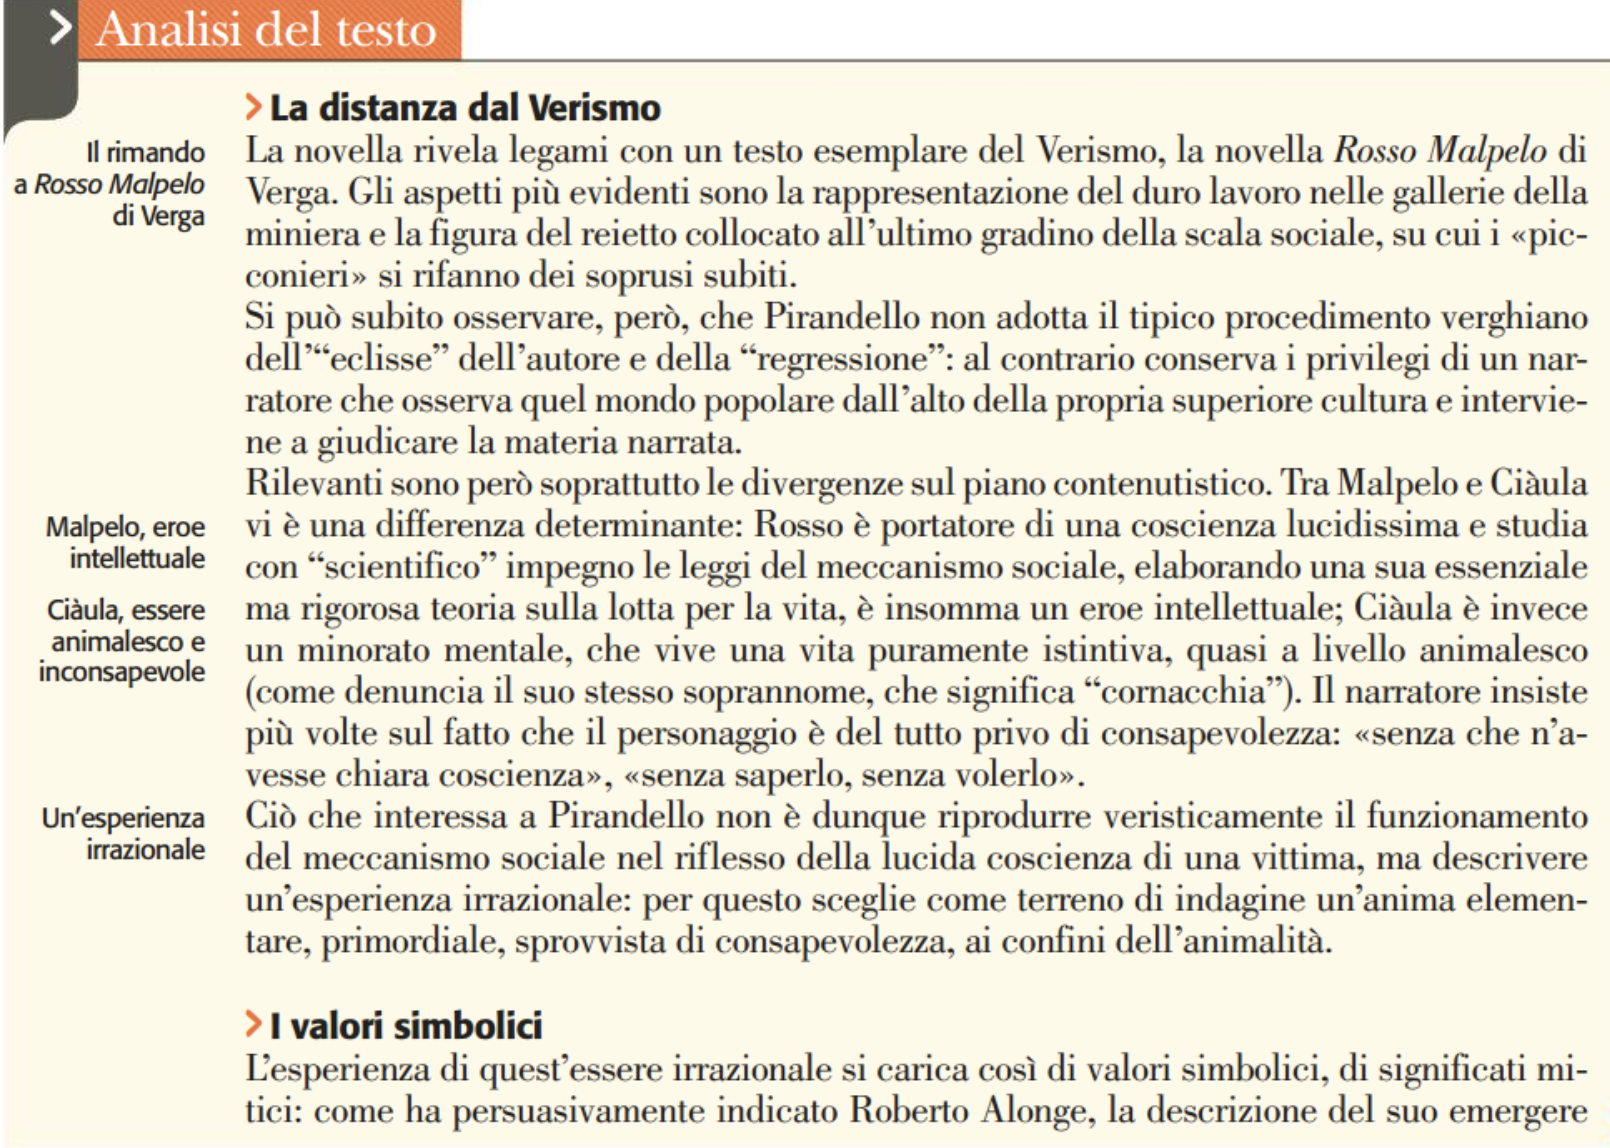
\includegraphics[width=\textwidth]{ciaula1}
\end{center}

\begin{center}
\includegraphics[width=\textwidth]{ciaula2}
\end{center}

\begin{center}
\includegraphics[width=\textwidth]{ciaula3}
\end{center}
\vfill

\chapter{Saggio: \textit{L'umorismo}}

Scritto intorno al 1908, anche se pubblicato nel 1920.

Si divide in due parti.

Nella \textbf{prima parte} Pirandello da delle indicazioni sul termine \textit{umorismo}, e l'umoristica è un'arte che in letteratura si trova in ogni epoca.

Nella \textbf{seconda parte} egli ci spiega cos'è l'umorismo.

La realtà non è più una realtà oggettiva. La realtà è molto differente da ciò che sta sotto, e che non appare.

L'arte non corrisponde più a canoni di bellezza, di perfezione formale. L'arte avrà il compito di oltrepassare l'apparenza per poter capire. L'arte deve insinuare il dubbio, e solo sul dubbio si può iniziare a ragionare.

Nel saggio c'è un paragone con una situazione che serve a far capire l'atteggiamento umoristico (che non è comico): fa l'esempio della donna anziana, truccata in modo esagerata e volgare; vedendo una donna così conciata si può avvertire un senso di comicità: si avverte che quello che noi vediamo è esattamente il contrario di quello che dovrebbe essere. Se però andiamo oltre all'apparenza, e scopriamo che lei si concia così per mantenere l'attenzione del marito molto più giovane di lei, e che ha paura di perdere, ecco che noi andiamo a scoprire la verità di quell'individuo, che è molto dolorosa.

Pirandello riporta un esempio letterario: Don Chisciotte: oltre la superficie è una persona alienata, che non è come vorrebbe essere, che soffre e finisce sempre perdente.

\section{T: \textit{Un'arte che scompone il reale}}

\subsection*{Righe 26-38}

\begin{quotation}
Vedo una vecchia signora, coi capelli ritinti, tutti unti non si sa di quale orribile manteca, e poi tutta goffamente imbellettata e parata d’abiti giovanili. Mi metto a ridere. Avverto che quella vecchia signora è il contrario di ciò che una vecchia rispettabile signora dovrebbe essere. Posso così, a prima giunta e superficialmente, arrestarmi a questa impressione comica. Il comico è appunto un avvertimento del contrario. Ma se ora interviene in me la riflessione, e mi suggerisce che quella vecchia signora non prova forse nessun piacere a pararsi così come un pappagallo, ma che forse ne soffre e lo fa soltanto perché pietosamente s’inganna che parata così, nascondendo così le rughe e la canizie, riesca a trattenere a sé l’amore del marito molto più giovane di lei, ecco che io non posso più riderne come prima, perché appunto la riflessione, lavorando in me, mi ha fatto andar oltre a quel primo avvertimento, o piuttosto, più addentro: da quel primo avvertimento del contrario mi ha fatto passare a questo sentimento del contrario. Ed è tutta qui la differenza tra il comico e l’umoristico
\end{quotation}

\subsection*{Righe 65-94}

\begin{quotation}
La vita è un flusso continuo che noi cerchiamo d’arrestare, di fissare in forme stabili e determinate, dentro e fuori di noi, perchè noi già siamo forme fissate, forme che si muovono in mezzo ad altre immobili, e che però possono seguire il flusso della vita, fino a tanto che, irrigidendosi man mano, il movimento, già a poco a poco rallentato, non cessi. Le forme, in cui cerchiamo d’arrestare, di fissare in noi questo flusso continuo, sono i concetti, sono gli ideali a cui vorremmo serbarci coerenti, tutte le finzioni che ci creiamo, le condizioni, lo stato in cui tendiamo a stabilirci. Ma dentro di noi stessi, in ciò che noi chiamiamo anima, e che è la vita in noi, il flusso continua, indistinto, sotto gli argini, oltre i limiti che noi imponiamo, componendoci una coscienza, costruendoci una personalità. In certi momenti tempestosi, investite dal flusso, tutte quelle nostre forme fittizie crollano miseramente; e anche quello che non scorre sotto gli argini e oltre i limiti, ma che si scopre a noi distinto e che noi abbiamo con cura incanalato nei nostri affetti, nei doveri che ci siamo imposti, nelle abitudini che ci siamo tracciate, in certi momenti di piena straripa e sconvolge tutto.

Vi sono anime irrequiete, quasi in uno stato di fusione continua, che sdegnano di rapprendersi, d’irrigidirsi in questa o in quella forma di personalità. Ma anche per quelle più quiete, che si sono adagiate in una o in un’altra forma, la fusione è sempre possibile: il flusso della vita è in tutti.

E per tutti però può rappresentare talvolta una tortura, rispetto all’anima che si muove e si fonde, il nostro stesso corpo fissato per sempre in fattezze immutabili. Oh perchè proprio dobbiamo essere così, noi? — ci domandiamo talvolta allo specchio, — con questa faccia, con questo corpo? — Alziamo una mano, nell’incoscienza; e il gesto ci resta sospeso. Ci pare strano che l’abbiamo fatto noi. \textit{Ci vediamo vivere.} [\dots]

Da quanto abbiamo detto finora intorno alla speciale attività della riflessione nell’umorista, appare chiaramente che diverso per forza deve essere il procedimento dell’arte umoristica rispetto a quello dell’arte in genere.

Anch’essa l’Arte, come tutte le costruzioni ideali o illusorie, tende a fissar la vita: la fissa in un momento o in varii momenti determinati: la statua in un gesto, il paesaggio in un aspetto temporaneo, immutabile. Ma, e la perpetua mobilità degli aspetti successivi? e la fusione continua in cui le anime si trovano?
\end{quotation}

L'individuo vive di questa vita, ma ha necessità di una forma, ed è lui a costruirsi la forma entro cui soffoca: la forma come una maschera ci chiude e ci fissa; la forma sono le trappole (matrimonio, situazione economica, leggi, situazioni, vincoli sociali): l'uomo ha bisogno di rispondere ad una forma.
La prima che ci danno, quando nasciamo, è il nome. L'unico personaggio di Pirandello che riesce a liberarsi anche del nome è il protagonista di \textit{Uno, nessuno e Centomila}, che in questa situazione di pazzia delle ultime pagine del libro si trova addirittura senza nome.

Anche quando Mattia Pascal resta privo di questa forma, a poco a poco si ricostruisce questa forma: pensa ad un nuovo nome, pensa ad uno stato sociale: l'uomo ha necessità, e gli altri hanno necessità di creare su quell'individuo delle personalità, che sono le varie maschere che indossiamo nei vari ambiti in cui ci troviamo.

La letteratura non può fissare con i canoni classici di perfezione di bellezza: non può che essere paradossale.

\subsection*{Righe 95-108}

\begin{quotation}
L’arte, in genere, compone; l’umorismo decompone.

L’arte astrae e concentra, coglie cioè e rappresenta così degli individui come delle cose, l’idealità essenziale e caratteristica. Ora pare all’umorista che tutto ciò semplifichi troppo la natura e tenda a rendere troppo ragionevole o almeno troppo coerente la vita. Gli pare che delle cause, delle cause vere che muovono spesso questa povera anima umana a gli atti più inconsulti, assolutamente imprevedibili, l’arte in genere non tenga quel conto che secondo lui dovrebbe. Per l’umorista le cause, nella vita, non sono mai così logiche, così ordinate, come nelle nostre comuni opere d’arte, in cui tutto è, in fondo, combinato, congegnato, ordinato ai fini che lo scrittore s’è proposto. L’ordine? la coerenza? Ma se noi abbiamo dentro quattro, cinque anime in lotta fra loro: l’anima istintiva, l’anima morale, l’anima affettiva, l’anima sociale? E secondo che domina questa o quella, s’atteggia la nostra coscienza; e noi riteniamo valida e sincera quella interpretazione fittizia di noi medesimi, del nostro essere interiore che ignoriamo, perchè non si manifesta mai tutt’intero, ma ora in un modo, ora in un’altro, come volgano i casi della vita.
\end{quotation}

\begin{center}
\includegraphics[width=\textwidth]{umorismo1}
\end{center}

\begin{center}
\includegraphics[width=\textwidth]{umorismo2}
\end{center}

\begin{center}
\includegraphics[width=\textwidth]{umorismo3}
\end{center}

\chapter{T: \textit{Il treno ha fischiato}}

Il termine \textit{masca} in piemontese significa "strega".

Il protagonista è un impiegato. Molti letterati hanno vissuto questa esperienza dell'impiegato.

I termini iniziali indica il fallimento della mania positivistica di voler dare una spiegazione scientifica a tutto: abbiamo una serie di termini scientifici, all'inizio della novella (in \textit{medias res}).
Nonostante questo nessuno riesce a darsi spiegazioni di quello che abbia fatto il protagonista, soprattutto una spiegazione scientifica.

Belluca è il protagonista della novella.

C'è un narratore che ci guida un po'.

Il protagonista è un individuo, che ha una maschera: quella di un uomo \textit{mansueto, metodico e paziente}; i colleghi e il capoufficio lo conoscono così

Ci sono degli aggettivi, quali "specialissime", "naturalissimo": naturalissimo è la routine in cui si muove questo personaggio, che è di un certo tipo. In questa routine il personaggio ha questa maschera. La sua reazione è la cosiddetta \textbf{coda del mostro}: si prende per assurdo un comportamento, ma solo perché si vede solo una parte, e non anche quello che sta dietro (la coda appunto).

\elenco{\item \textbf{riga 54}: La rivelazione e l'epifania c'è già stata, ma gli altri non lo sanno. Il sorriso è un segno esteriore di questa rivelazione.
\item \textbf{riga 56}: Anche la sua espressione non gli si confà: lui ha avuto la sua epifania, e tutti i suoi atteggiamenti fanno crollare le certezze degli altri: non ci sono nessi causali, non c'è una realtà oggettiva. Si dissolve la maschera di Belluca (che hanno costruito gli altri): c'è una pluralità prospettica.
}

Il fatto epifanico è quell'avvenimento che giunge improvviso: sono delle azioni e dei fatti che sono completamente insignificanti, a volte un po' strani. Per esempio, il treno ha fischiato (\textbf{riga 60}) per Belluca
Per gli altri, questo è sintomo di pazzia.

Il fatto epifanico è qualcosa che squarcia il grigiore della trappola in cui si trova Belluca: nel suo caso la trappola è costituita dalla famiglia, e da tutte quelle regole che ci sono in ufficio. L'evento squarcia questa realtà, squarcia la forma.

Pensando ad un individuo che ha avuto la vita limitata sempre da una forma, che ad un certo punto viene a mancare, si può immaginare che la vita sgorghi tutta improvvisamente: ci sono degli eccessi.
È difficile regolarsi dopo aver perduto la forma, così come è difficile rientrare nella forma, quasi doloroso

\elenco{\item \textbf{riga 67}: \textit{giù risate da pazzi}: la prima reazione, come ci dice ne \textit{L'umorismo}, è quella di ilarità; dopo, si avverte il sentimento del contrario, e a questo punto subentra dolore; tra poco il narratore ci spiegherà la trappola di Belluca, e noi capiremo come non ci sia nulla da ridere della sua situazione
\item \textbf{righe 73-74}: dopo essersi liberati della forma è difficile sottostargli di nuovo
\item \textbf{righe 88-90}: Questa cosa è assurda per tutto coloro che non conoscono la vera vita di Belluca. Il narratore, abbastanza attendibile, conosce la situazione di Belluca, è il meglio informato sui fatti, e lui non si stupisce.
}

L'assurdità della vita funziona come un contesto in cui quello che si inserisce ha un significato.
La \textbf{coda del mostro} è mostruosa se la separiamo dal resto del mostro, ma se la riattacchiamo al corpo questa coda non è mostruosa, ma naturale.
La vita assurda che conduce Belluca è il contesto in cui quello che è capitato non appare più come assurdo.

\elenco{\item \textbf{riga 91}: il narratore non ride, c'è il sentimento del contrario, si va oltre al comico.
\item \textbf{righe 109-122}: è già scattato il sentimento del contrario, con la descrizione della situazione. LE tre cieche vanno a contrapporsi alla luce epifanica di Belluca
\item \textbf{righe 151-178}: flusso di coscienza: è l'immagine lampante di quel sentimento e di quella vita che sta balzando fuori dalla forma, un flusso che non si può controllare e che si esprime verbalmente attraverso il flusso di coscienza (non tiene conto delle regole della sintassi tradizionale).
\item \textbf{riga 183}: si fa fatica a rientrare nella forma, \textit{ha ecceduto}
}

Il finale esprime una sorta di ottimismo.

Tutte le novelle di Pirandello sono raccolte nel testo \textit{Novelle per un anno}

\includepdf{page917.png}
\includepdf{page918.png}
\includepdf{page919.png}
\includepdf{page920.png}
\includepdf{page921.png}
\includepdf{page922.png}

\chapter{Altri romanzi}

\section{\textit{L'esclusa}}

È il primo romanzo di Pirandello, pubblicato nel 1901.

È una vicenda che si svolge in Sicilia; a prima vista sembra che l'ambientazione sia un po' quella delle novelle Verghiane. In realtà non è così.

Questo romanzo, per ambientazione, personaggi e alcune tematiche fa pensare alle ambientazioni veriste: ci troviamo in Sicilia, in un contesto modesto; di fatto la vicenda va in tutt'altra direzione: non abbiamo l'esigenza dell'autore di mostrarci una realtà in cui i deboli vengono sopraffatti, ma all'autore interessa l'\textbf{assurdità della vita}

La vicenda è paradossale: Marta è una giovane donna, sposata, maestra: viene accusata di adulterio dal marito, adulterio che lei non ha commesso. Nel momento in cui il marito l'accusa di adulterio, per tutti è adulterio, anche per i familiari (tranne la madre e la sorella).

L'\emph{ambientazione} ha una sua importanza, ma non è questo che interessa a Pirandello: è molto più importante \textbf{ciò che appare} rispetto a ciò che è

Ci sono diverse peripezie: perde il figlio che aveva in grembo, è costretta a cambiare città, e riesce a rifarsi una vita.
Incontra l'uomo che si pensava fosse il suo amante, e lo diventa veramente.
Ad un certo punto la suocera è in fin di vita, e lei corre al suo capezzale. La suocera è emblematica, perché anche lei era stata accusata di adulterio.
Al capezzale della suocera, il marito di Marta le chiede di tornare insieme, proprio quando lei è veramente colpevole.

Quando era innocente per la società era colpevole, mentre quando è davvero colpevole viene perdonata.

\section{\textit{Il turno}}

Il gioco del caso è ancora ripreso nel breve romanzo successivo, \textit{Il turno} (1895), dove un innamorato deve aspettare il suo "turno" per sposare la donna amata, dopo la morte di altri due mariti. Il tema è però impostato a livello di minore responsabilità intellettuale, come divertimento comico, dai risvolti bizzarri, grotteschi, quasi marionettistici.

\section{\textit{I vecchi e i giovani}}

È un romanzo sociale di ambientazione siciliana. È la Sicilia dei sanguinosi moti dei Fasci siciliani del 1893, sconvolta dalle lotte di classe, con i clericali da un lato, tesi ad impedire il consolidamento del nuovo regime liberale, e la classe dirigente dall'altro, che disperde nel disordine morale i sacrifici e i meriti acquisiti.

Più che casi individuali, i personaggi del romanzo interpretano i diversi aspetti della complessa situazione storica che stanno vivendo.

Così il principe don Ippolito di Colimbetra, fedele suddito borbonico; don Flaminio Salvo, esponente della nuova borghesia capitalista; Roberto Auriti, glorioso garibaldino che si spegne in un'esistenza amorfa; il giovane principe Gerlando di Colimbetra, sostenitore delle nuove idee e per questo costretto all'esilio.

I personaggi rappresentano un contrasto di concezioni e di ideali che si risolve nel contrasto tra due generazioni: quella che ha fatto l'Unità e che vede perduta l'eredità del Risorgimento, e quella più giovane, che nel gretto conservatorismo dei padri scorge solo la difesa di interessi reazionari.

Ne I vecchi e i giovani l'autore esprime un giudizio storico molto severo sul processo di riunificazione dell'Italia e dello stato nato da essa. Non a caso Carlo Salinari, analizzando questo romanzo, parla di tre “fallimenti collettivi” riferendosi al Risorgimento, come mancato moto generale di rinnovamento dell'Italia; all'unità, come fallito strumento di liberazione e di sviluppo delle zone più arretrate e in particolare della Sicilia e dell'Italia meridionale; e al socialismo, che avrebbe potuto essere la ripresa del movimento risorgimentale. Questi fallimenti si sovrappongono poi a quelli “individuali” «dei vecchi che non hanno saputo passare dagli ideali alla realtà e si trovano a essere responsabili degli scandali, della corruzione e del malgoverno dei giovani».

Nell'ultimo capitolo della seconda parte del romanzo, don Cosmo, il fratello intellettuale di Ippolito, fornisce la chiave di lettura degli avvenimenti e il punto di vista di Pirandello, nel corso della conversazione con Gerlando:

\citazione{«Una cosa è triste, cari miei: aver capito il gioco! Dico il gioco di questo demoniaccio beffardo che ciascuno di noi ha dentro e che si spassa a rappresentarci di fuori, come realtà, ciò che poco dopo egli stesso ci scopre come una nostra illusione, deridendoci degli affanni che per essa ci siamo dati, e deridendoci anche, come avviene a me, del non averci saputo illudere, poiché fuori di queste illusioni non c'è più altra realtà...»}

Questo romanzo riprende i temi giovanili, ed è un romanzo storico.

Mostra due generazioni a confronto, e riprende le idee del periodo giovanile di Pirandello, con forti ideali patriottici.

In questo romanzo mette a confronto due generazioni: i vecchi sono quelli che hanno fatto il risorgimento italiano, e i giovani sono quelli che vanno a deludere le aspettative del risorgimento; rappresentano la disillusione che segue a questo processo di unità


\chapter{\textit{Il fu Mattia Pascal}}

La società presenta delle trappole: Mattia Pascal ha delle trappole ben definite: oltre alle convenzioni, ha una trappola costituita dal contesto familiare (moglie e suocera): la famiglia, tanto agognata da Pascoli, è vissuta da Pirandello come una trappola, come qualcosa che imprigiona.
Così, insieme alla famiglia, c'è anche il contesto economico di Mattia Pascal (i suoi debiti).

Mattia Pascal ad un certo punto si libera da queste trappole, privato di forma: lui scappa di casa, e va a Montecarlo: qui vive una avventura incredibile: va a giocare al casinò e vince tantissimi soldi, da star bene tutta la vita.
Lui decide di tornare a casa, e mentre torna a casa legge la notizia della sua morte suicida (riconosciuto da Moglie e Suocera).

Lui appena letta la notizia si arrabbia: ad un certo punto è illuminato da una intuizione: lui in quel momento ha solo la vita e non la forma; Mattia Pascal per la legge non esiste più: lui è al di fuori, ha una posizione estraniata rispetto alla sua vecchia vita. Non ritornerà a casa.

Pirandello ci dice che l'uomo ha bisogno della Forma, e quindi questo è proprio quello che succederà a Mattia Pascal.

Il romanzo è pubblicato nel 1904: questo è un periodo molto particolare, che segue il disastro economico che si cala sulla famiglia, e che fa peggiorare la situazione mentale della moglie.
Il libro è scritto proprio mentre Pirandello è al capezzale della moglie.

L'opera risente moltissimo di questo contesto, e tutta l'opera di Pirandello è influenzata dalla tematica della \textbf{pazzia} (Vedasi \textit{Il treno ha fischiato})

Il tema della pazzia in questo romanzo non è rappresentato direttamente, ma è rappresentata come qualcosa che aliena e che estranea, e che forse anche preserva.
Mattia Pascal è un \emph{forestiere della vita}

È la storia paradossale di un piccolo borghese, imprigionato come sempre nella trappola di una famiglia insopportabile e di una misera condizione sociale, che, per un caso fortuito, si trova improvvisamente libero e padrone di sé: diviene economicamente autosufficiente grazie ad una cospicua vincita al casino di Montecarlo e apprende di essere ufficialmente morto, in quanto la moglie e la suocera lo hanno riconosciuto nel cadavere di un annegato. Però, invece di approfittare della liberazione dalla forma sociale per vivere immerso nel fluire della vita, senza più assumere maschere, Mattia Pascal si sforza di costruirsi un'identità nuova. In lui resta insuperabile l'attaccamento alla vita sociale, alla trappola, quindi egli soffre perché la sua identita falsa lo costringe all'esclusione dalla vita degli altri. Decide pertanto di rientrare nella sua vecchia identità, tornando in famiglia, ma scopre che la moglie si è risposata ed ha avuto una figlia da un altro. Non gli resta dunque che adattarsi alla sua condizione sospesa di "forestiere della vita", che contempla gli altri dall'esterno, consapevole di non essere più "nessuno".

Quando la forma si rompe, ne sgorga la vita. Mattia Pascal decide di godersi la vita: inizia a viaggiare.
Mattia Pascal incorre in un errore: non è ancora filosofo, come il protagonista di \textit{Uno, Nessuno e Centomila}; liberatosi della forma, ad un certo punto ne sente la necessità. Si crea una \textbf{forma fittizia}.
Inizia con una serie di modifiche che partono dall'aspetto esteriore: si taglia la barba, etc etc.
Poi si costruisce una nuova identità: si chiamerà Adriano Meis e si costruisce un passato fittizio.

Inizia una nuova vita, e vuole una casa: non vuole più stare in una camera d'albergo, senza oggetti suoi.

Si rende conto che anche la vita senza una forma non può essere vita vera. Sente quindi la \textbf{necessità di questa forma}.
Si reca a Roma, va da un affittacamere, che è un po' un filosofo, ed è fissato dalle sedute spiritiche.
C'è la figlia dell'affittacamere, l'ombra della sorella di lei, e il marito vedovo di quest'ultima.

Lui si innamora della figlia, \emph{Adriana}, ma col passare del tempo si rende conto che non può vivere senza la forma. Un passaggio significativo è il seguente: è per strada, vede la sua ombra, e tutti possono calpestare la sua \textbf{ombra}: si rende conto che lui è un'ombra, e tutti lo possono calpestare.

Inscena quindi un \emph{suicidio} e decide di ritornare alla sua vecchia vita. Pensa di poter ritornare nella sua vecchia forma.

Anche quella che era considerata una trappola non c'è più: la moglie si è risposata, ha avuto altri figli, e gli è solo consentito di ritornare nella dimensione del lavoro.


Il finale di questo testo ci mostra quello che il personaggio definisce il \textbf{forestiere della vita}: Mattia Pascal è in una posizione straniata, vede la vita dal di fuori. È lo stesso tipo di straniamento di Belluca, ma è forzato.
Lui ha fatto l'errore di voler tornare nella forma, e viene soffocato prima dalla forma fittizia e poi dall'impossibilità di tornare nella forma originale.

\section{T: \textit{La costruzione della nuova identità e la sua crisi}}

\subsection*{Righe 10-62}

Sia all'inizio del romanzo, quando Mattia Pascal si trova pieno di soldi e morto per lo stato.

Egli cade subito nell'errore di volersi ricostruire una nuova forma: dapprima riguarda l'aspetto fisico, ma poi riguarda il nome e l'identità.

\begin{quotation}
Ero solo ormai, e più solo di com’ero non avrei potuto essere su la terra, sciolto nel presente d’ogni legame e d’ogni obbligo, libero, nuovo e assolutamente padrone di me, senza più il fardello del mio passato, e con l’avvenire dinanzi, che avrei potuto foggiarmi a piacer mio.

Ah, un pajo d’ali! Come mi sentivo leggero!

Il sentimento che le passate vicende mi avevano dato della vita non doveva aver più per me, ormai, ragion d’essere. Io dovevo acquistare un nuovo sentimento della vita, senza avvalermi neppur minimamente della sciagurata esperienza del fu Mattia Pascal.

Stava a me: potevo e dovevo esser l’artefice del mio nuovo destino, nella misura che la Fortuna aveva voluto concedermi.

— E innanzi tutto, — dicevo a me stesso, — avrò cura di questa mia libertà: me la condurrò a spasso per vie piane e sempre nuove, nè le farò mai portare alcuna veste gravosa. Chiuderò gli occhi e passerò oltre appena lo spettacolo della vita in qualche punto mi si presenterà sgradevole. Procurerò di farmela più tosto con le cose che si sogliono chiamare inanimate, e andrò in cerca di belle vedute, di ameni luoghi tranquilli. Mi darò a poco a poco una nuova educazione; mi trasformerò con amoroso e paziente studio, sicchè, alla fine, io possa dire non solo di aver vissuto due vite, ma d’essere stato due uomini.

Già ad Alenga, per cominciare, ero entrato, poche ore prima di partire, da un barbiere, per farmi accorciar la barba: avrei voluto levarmela tutta, lì stesso, insieme coi baffi; ma il timore di far nascere qualche sospetto in quel piccolo paese mi aveva trattenuto.

Il barbiere era anche sartore, vecchio, con le reni quasi ingommate dalla lunga abitudine di star curvo, sempre in una stessa positura, e portava gli occhiali su la punta del naso. Più che barbiere doveva esser sartore. Calò come un flagello di Dio su quella barbaccia che non m’apparteneva più, armato di certi forbicioni da maestro di lana, che avevan bisogno d’esser sorretti in punta con l’altra mano. Non m’arrischiai neppure a fiatare: chiusi gli occhi, e non li riaprii, se non quando mi sentii scuotere pian piano.

Il brav’uomo, tutto sudato, mi porgeva uno specchietto perchè gli sapessi dire se era stato bravo.

Mi parve troppo!

— No, grazie, — mi schermii. — Lo riponga. Non vorrei fargli paura.

Sbarrò tanto d’occhi, e:

— A chi? — domandò.

— Ma a codesto specchietto. Bellino! Dev’essere antico...

Era tondo, col manico d’osso intarsiato: chi sa che storia aveva e donde e come era capitato lì, in quella sarto-barbieria. Ma infine, per non dar dispiacere al padrone, che seguitava a guardarmi stupito, me lo posi sotto gli occhi.

Se era stato bravo!

Intravidi da quel primo scempio qual mostro fra breve sarebbe scappato fuori dalla necessaria e radicale alterazione dei connotati di Mattia Pascal. Ed ecco una nuova ragione d’odio per lui! Il mento piccolissimo, puntato e rientrato, ch’egli aveva nascosto per tanti e tanti anni sotto quel barbone, mi parve un tradimento. Ora avrei dovuto portarlo scoperto, quel cosino ridicolo! E che naso mi aveva lasciato in eredità! E quell’occhio!

— Ah, quest’occhio, — pensai, — così in estasi da un lato, rimarrà sempre suo nella mia nuova faccia! Io non potrò far altro che nasconderlo alla meglio dietro un pajo d’occhiali colorati, che coopereranno, figuriamoci, a rendermi più amabile l’aspetto. Mi farò crescere i capelli e, con questa bella fronte spaziosa, con gli occhiali e tutto raso, sembrerò un filosofo tedesco. Finanziera e cappellaccio a larghe tese.

Non c’era via di mezzo: filosofo dovevo essere per forza con quella razza d’aspetto. Ebbene, pazienza: mi sarei armato d’una discreta filosofia sorridente per passare in mezzo a questa povera umanità, la quale, per quanto avessi in animo di sforzarmi, mi pareva difficile che non dovesse più parermi un po’ ridicola e meschina.
\end{quotation}

\subsection*{Righe 71-74}

\begin{quotation}
La fortuna mi aveva sciolto di ogni intrico, all’improvviso, mi aveva sceverato dalla vita comune, reso spettatore estraneo della briga in cui gli altri si dibattevano ancora, e mi ammoniva dentro:

— Vedrai, vedrai com’essa t’apparirà curiosa, ora, a guardarla così da fuori!
\end{quotation}

\subsection*{Righe 75-99}

\begin{quotation}
In fondo, ero già un po’ stanco di quell’andar girovagando sempre solo e muto. Istintivamente cominciavo a sentir il bisogno di un po’ di compagnia. Me ne accorsi in una triste giornata di novembre, a Milano, tornato da poco dal mio giretto in Germania.

Faceva freddo, ed era imminente la pioggia, con la sera. Sotto un fanale scorsi un vecchio cerinajo, a cui la cassetta, che teneva dinanzi con una cinta a tracolla, impediva di ravvolgersi bene in un logoro mantelletto che aveva su le spalle. Gli pendeva dalle pugna strette sul mento un cordoncino, fino ai piedi. Mi chinai a guardare e gli scoprii tra le scarpacce rotte un cucciolotto minuscolo, di pochi giorni, che tremava tutto di freddo e gemeva continuamente, lì rincantucciato. Povera bestiolina! Domandai al vecchio se la vendesse. Mi rispose di sì e che me l’avrebbe venduta anche per poco, benchè valesse molto: ah, si sarebbe fatto un bel cane, un gran cane, quella bestiola:

— Venticinque lire...

Seguitò a tremare il povero cucciolo, senza inorgoglirsi punto di quella stima: sapeva di certo che il padrone con quel prezzo non aveva affatto stimato i suoi futuri meriti, ma la imbecillità che aveva creduto di leggermi in faccia.

Io intanto, avevo avuto il tempo di riflettere che, comprando quel cane, mi sarei fatto, sì, un amico fedele e discreto, il quale per amarmi e tenermi in pregio non mi avrebbe mai domandato chi fossi veramente e donde venissi e se le mie carte fossero in regola; ma avrei dovuto anche mettermi a pagare una tassa: io che non ne pagavo più! Mi parve come una prima compromissione della mia libertà, un lieve intacco ch’io stessi per farle.
\end{quotation}

\subsection*{Righe 136-144}

\begin{quotation}
Ma una casa, una casa mia, tutta mia, avrei potuto averla io più? I miei denari erano pochini... Ma una casettina modesta, di poche stanze? Piano: bisognava vedere, considerar bene prima, tante cose. Certo, libero, liberissimo, io potevo essere soltanto così, con la valigia in mano: oggi qua, domani là. Fermo in un luogo, proprietario d’una casa, eh, allora: registri e tasse subito! E non mi avrebbero iscritto all’anagrafe? Ma sicuramente! E come? con un nome falso? E allora, chi sa?, forse indagini segrete intorno a me da parte della polizia... Insomma, impicci, imbrogli!... No, via: prevedevo di non poter più avere una casa mia, oggetti miei. Ma mi sarei allogato a pensione in qualche famiglia, in una camera mobiliata. Dovevo affliggermi per così poco?
\end{quotation}

\subsection*{Righe 202-215}

\begin{quotation}
Ora, se questo Adriano Meis non aveva il coraggio di dir bugie, di cacciarsi in mezzo alla vita, e si appartava e rientrava in albergo, stanco di vedersi solo, in quelle tristi giornate d’inverno, per le vie di Milano, e si chiudeva nella compagnia del morto Mattia Pascal, prevedevo che i fatti miei, eh, avrebbero cominciato a camminar male, che insomma non mi s’apparecchiava un divertimento, e che la mia bella fortuna, allora...

Ma la verità forse era questa: che nella mia libertà sconfinata, mi riusciva difficile cominciare a vivere in qualche modo. Sul punto di prendere una risoluzione, mi sentivo come trattenuto, mi pareva di vedere tanti impedimenti e ombre e ostacoli.

Ed ecco, mi cacciavo, di nuovo, fuori, per le strade, osservavo tutto, mi fermavo a ogni nonnulla, riflettevo a lungo su le minime cose; stanco, entravo in un caffè, leggevo qualche giornale, guardavo la gente che entrava e usciva; alla fine, uscivo anch’io. Ma la vita, a considerarla così, da spettatore estraneo, mi pareva ora senza costrutto e senza scopo; mi sentivo sperduto tra quel rimescolìo di gente. E intanto il frastuono, il fermento continuo della città m’intronavano.
\end{quotation}

\begin{center}
\includegraphics[width=\textwidth]{identita1}
\end{center}
\vfill
\begin{center}
\includegraphics[width=\textwidth]{identita2}
\end{center}

\begin{center}
\includegraphics[width=\textwidth]{identita3}
\end{center}

\begin{center}
\includegraphics[width=\textwidth]{identita4}
\end{center}

\section{T: \textit{Lo strappo nel cielo di carta}}

Mattia ha appena fatto l’operazione all’occhio, ed è cieco. Questo è significativo.

Il signor Paleari gli parla di un teatrino che sta per essere messo in atto, l’Oreste di Sofocle.

Oreste è figlio di Agamennone, ed è piccolo quando avviene l’omicidio del padre. Va via dalla reggia, e ritorna a 18 anni per vendicare la morte del padre, con l’aiuto di Elettra, sua sorella. Uccidono Egisto e Clitemnestra, assassini di Agamennone

Il signor Paleari spiega la differenza tra Oreste e Amleto. Oreste è un eroe tragico, senza ripensamento, mentre Amleto è un eroe moderno, con molti ripensamenti.

Il signor Paleari descrive come sarà il teatrino delle marionette e dice "se ci fosse uno strappo in questo cielo di carta le marionette non saprebbero più cosa fare". Il teatrino è un mondo fittizio,  ma le marionette non lo sanno, per le marionette è vero.
Questa immagine serve al Paleari per spiegare la sua teoria della \textbf{lanterninosofia}; la lanterna costituisce i grandi ideali come religione, patria, legge... se questi ideali vanno in crisi, quindi se lanterna si spegne, l'individuo non ha più punti di riferimento e non sa più cosa fare.
Secondo Pirandello il primo momento in cui ogni ideale va in crisi nella storia dell'uomo è la scoperta copernicana, gli uomini non hanno più punti di riferimento certi e quindi vanno in crisi.

\subsection*{Righe 1-19}

\begin{quotation}
— La tragedia d’Oreste in un teatrino di marionette! — venne ad annunziarmi il signor Anselmo Paleari. — Marionette automatiche, di nuova invenzione. Stasera, alle ore otto e mezzo, in via dei Prefetti, n. 54. Sarebbe da andarci, signor Meis.

— La tragedia d’Oreste?

— Già! D’après Sophocle, dice il manifestino. Sarà l’Elettra. Ora senta un po’ che bizzarria mi viene in mente! Se, nel momento culminante, proprio quando la marionetta che rappresenta Oreste è per vendicare la morte del padre sopra Egisto e la madre, si facesse uno strappo nel cielo di carta del teatrino, che avverrebbe? Dica lei.

— Non saprei, — risposi, stringendomi ne le spalle.

— Ma è facilissimo, signor Meis! Oreste rimarrebbe terribilmente sconcertato da quel buco nel cielo.

— E perchè?

— Mi lasci dire. Oreste sentirebbe ancora gl’impulsi della vendetta, vorrebbe seguirli con smaniosa passione, ma gli occhi, sul punto, gli andrebbero lì, a quello strappo, donde ora ogni sorta di mali influssi penetrerebbero nella scena, e si sentirebbe cader le braccia. Oreste, insomma, diventerebbe Amleto. Tutta la differenza, signor Meis, fra la tragedia antica e la moderna consiste in ciò, creda pure: in un buco nel cielo di carta.

E se ne andò, ciabattando.
\end{quotation}

L’identità è falsa, ma è il parametro che ci consente di sapere cosa dobbiamo fare e cosa dobbiamo essere. Se si crea lo strappo nel cielo di carta (che è un po’ come il treno del treno ha fischiato) si rompe la forma, e l’individuo non sa più come fare.
Nel mondo moderno alcune teorie hanno messo in crisi l’uomo moderno, distruggendo le sue certezze

\subsection*{Righe 44-58}

\begin{quotation}
E il signor Anselmo, seguitando, mi dimostrava che, per nostra disgrazia, noi non siamo come l’albero che vive e non si sente, a cui la terra, il sole, l’aria, la pioggia, il vento, non sembra che sieno cose ch’esso non sia: cose amiche o nocive. A noi uomini, invece, nascendo, è toccato un tristo privilegio: quello di sentirci vivere, con la bella illusione che ne risulta: di prendere cioè come una realtà fuori di noi questo nostro interno sentimento della vita, mutabile e vario, secondo i tempi, i casi e la fortuna.

E questo sentimento della vita per il signor Anselmo era appunto come un lanternino che ciascuno di noi porta in sè acceso; un lanternino che ci fa vedere sperduti su la terra, e ci fa vedere il male e il bene; un lanternino che projetta tutt’intorno a noi un cerchio più o meno ampio di luce, di là dal quale è l’ombra nera, l’ombra paurosa che non esisterebbe, se il lanternino non fosse acceso in noi, ma che noi dobbiamo pur troppo creder vera, fintanto ch’esso si mantiene vivo in noi. Spento alla fine a un soffio, ci accoglierà davvero quell’ombra fittizia, ci accoglierà la notte perpetua dopo il giorno fumoso della nostra illusione, o non rimarremo noi piuttosto alla mercè dell’Essere, che avrà soltanto rotto le vane forme della nostra ragione?
\end{quotation}

Il lanternino è un ideale in miniatura, quello della persona, individuali.
Pirandello ci parla di un’ombra nera che fa paura, che potrebbe essere la morte o lo stato che c’è prima di nascere.
Se si spegne il lanternino, noi abbiamo paura di questo nero, ma non dovrebbe essere così, perché noi il nero lo vediamo solo perché abbiamo acceso il lanternino.

\subsection*{Righe 82-83}

\begin{quotation}
Mi pare, signor Adriano, che noi ci troviamo adesso in uno di questi momenti. Gran bujo e gran confusione! Tutti i lanternoni, spenti. A chi dobbiamo rivolgerci?
\end{quotation}

\chapter{\textit{I quaderni di serafino Gubbio operatore}}

Questo romanzo è molto particolare.

Da un lato abbiamo l’operatore, Serafino, che è una sorta di cameraman, che filma e che è dietro una macchina e osserva. Vive al di fuori, un forestiere del mondo.
È un osservatore.

Dall’altro lui decide di scrivere questa storia dopo che è successo un qualcosa, che riguarda altri personaggi: una donna (femme fatale), un uomo innamorato di lei, e una fanciulla che è il tratto di unione tra le vicende degli attori e di Serafino (Serafino è innamorato di lei).

Dopo le vicende Serafino sarà muto.

Prima riusciva ad estraniarsi, a vivere da forestiere della vita. Poi si innamora della fanciulla, e questo fa “saltare” i suoi piani: è trascinato anche lui nella vita.

Il fatto che ha fatto diventare muto Serafino: l’uomo spara per davvero (sul palco) alla femme fatale, e la tigre presente sul set mangia l’uomo.
Questa vicenda è molto forzata.

\section{T: \textit{Viva la macchina che meccanizza la vita}}

\begin{quotation}
Soddisfo, scrivendo, a un bisogno di sfogo, prepotente. Scarico la mia professionale impassibilità e mi vendico, anche; e con me vendico tanti, condannati come me a non esser altro, che una mano che gira una manovella.

Questo doveva avvenire, e questo è finalmente avvenuto!

L'uomo che prima, poeta, deificava i suoi sentimenti e li adorava, buttati via i sentimenti, ingombro non solo inutile ma anche dannoso, e divenuto saggio e industre, s'è messo a fabbricar di ferro, d'acciajo le sue nuove divinità ed è diventato servo e schiavo di esse.

Viva la Macchina che meccanizza la vita!

Vi resta ancora, o signori, un po' d'anima, un po' di cuore e di mente? Date, date qua alle macchine voraci, che aspettano! Vedrete e sentirete, che prodotto di deliziose stupidità ne sapranno cavare.

Per la loro fame, nella fretta incalzante di saziarle, che pasto potete estrarre da voi ogni giorno, ogni ora, ogni minuto?

È per forza il trionfo della stupidità, dopo tanto ingegno e tanto studio spesi per la creazione di questi mostri, che dovevano rimanere strumenti e sono divenuti invece, per forza, i nostri padroni.

La macchina è fatta per agire, per muoversi, ha bisogno di ingojarsi la nostra anima, di divorar la nostra vita. E come volete che ce le ridiano, l'anima e la vita, in produzione centuplicata e continua, le macchine? Ecco qua: in pezzetti e bocconcini, tutti d'uno stampo, stupidi e precisi, da farne, a metterli sù, uno su l'altro, una piramide che potrebbe arrivare alle stelle. Ma che stelle, no, signori! Non ci credete. Neppure all'altezza d'un palo telegrafico. Un soffio li abbatte e li ròtola giù, e tal altro ingombro, non più dentro ma fuori, ce ne fa, che - Dio, vedete quante scatole, scatolette, scatolone, scatoline? - non sappiamo più dove mettere i piedi, come muovere un passo. Ecco le produzioni dell'anima nostra, le scatolette della nostra vita!

Che volete farci? Io sono qua. Servo la mia macchinetta, in quanto la giro perché possa mangiare. Ma l'anima, a me, non mi serve. Mi serve la mano; cioè serve alla macchina. L'anima in pasto, in pasto la vita, dovete dargliela voi signori, alla macchinetta ch'io giro. Mi divertirò a vedere, se permettete, il prodotto che ne verrà fuori. Un bel prodotto e un bel divertimento, ve lo dico io.

Già i miei occhi, e anche le mie orecchie, per la lunga abitudine, cominciano a vedere e a sentir tutto sotto la specie di questa rapida tremula ticchettante riproduzione meccanica.

Non dico di no: l'apparenza è lieve e vivace. Si va, si vola. E il vento della corsa dà un'ansia vigile ilare acuta, e si porta via tutti i pensieri. Avanti! Avanti perché non s'abbia tempo né modo d'avvertire il peso della tristezza, l'avvilimento della vergogna, che restano dentro, in fondo. Fuori, è un balenìo continuo, uno sbarbàglio incessante: tutto guizza e scompare.

Che cos'è? Niente, è passato! Era forse una cosa triste; ma niente, ora è passata.

C'è una molestia, però, che non passa. La sentite? Un calabrone che ronza sempre, cupo, fosco, brusco, sotto sotto, sempre. Che è? Il ronzìo dei pali telegrafici? lo striscìo continuo della carrùcola lungo il filo dei tram elettrici? il fremito incalzante di tante macchine, vicine, lontane? quello del motore dell'automobile? quello dell'apparecchio cinematografico?

Il bàttito del cuore non s'avverte, non s'avverte il pulsar delle arterie. Guaj, se s'avvertisse! Ma questo ronzìo, questo ticchettìo perpetuo, sì, e dice che non è naturale tutta questa furia turbinosa, tutto questo guizzare e scomparire d'immagini; ma che c'è sotto un meccanismo, il quale pare lo insegua, stridendo precipitosamente.

Si spezzerà?

Ah, non bisogna fissarci l'udito. Darebbe una smania di punto in punto crescente, un'esasperazione a lungo insopportabile; farebbe impazzire.

In nulla, più in nulla, in mezzo a questo tramenìo vertiginoso, che investe e travolge, bisognerebbe fissarsi. Cogliere, attimo per attimo, questo rapido passaggio d'aspetti e di casi, e via, fino al punto che il ronzìo per ciascuno di noi non cesserà.
\end{quotation}

Pirandello considera il cinema in maniera molto critica: questo brano ci consente di ripensare alla conclusione della coscienza di Zeno, dove Svevo immagina uno scenario di distruzione, in cui la macchina è l’unica evoluzione dell’uomo.

La modernità ha i suoi rumori.

\begin{center}
\includegraphics[width=\textwidth]{macchina1}
\end{center}

\begin{center}
\includegraphics[width=\textwidth]{macchina2}
\end{center}

\begin{center}
\includegraphics[width=\textwidth]{macchina3}
\end{center}

\begin{center}
\includegraphics[width=\textwidth]{macchina4}
\end{center}
\vfill
\begin{center}
\includegraphics[width=\textwidth]{macchina5}
\end{center}

\begin{center}
\includegraphics[width=\textwidth]{macchina6}
\end{center}
\vfill
\section{T: \textit{L'automobile e la carrozzella: la modernità e il passato}}

Vedasi pagine successive

\includepdf{page961.png}
\includepdf{page962.png}
\includepdf{page963.png}


\chapter{\textit{Uno, Nessuno e Centomila}}

Ultimo romanzo di Pirandello

È il romanzo maturo di Pirandello, dopodiché egli continuerà a scrivere prevalentemente drammi teatrali.

Sembra che Vitangelo Moscarda abbia compiuto un passo in avanti rispetto a Mattia Pascal, verso quella scelta che possa consentire una soluzione tra quel contrasto tra vita e forma, che non sembra poterne avere una.
Sembra che egli sia riuscito a rompere il vincolo ultimo (il primo a sancire l’essere formale dell’individuo), cioè il nome e il cognome.
Per quanto Mattia Pascal si è ridotto a forestiere della vita, di fatto lui era lì, vicino.
Fisicamente, invece, Vitangelo Moscarda, si separa dal consorzio degli uomini, e vive in questa sorta di ospizio.

Per un caso Vitangelo Moscarda scopre di vivere in tante maschere. È figlio di un banchiere (usuraio) che l’ha lasciato molto ricco, e non ha alcuna preoccupazione al mondo.
Si guarda allo specchio, e scopre dalla moglie di avere il naso storto: capisce che la moglie lo vede diversamente da come si vede lui.
Inizia una sorta di indagine, e si rende conto che lo vedono in tanti modi diversi.

Il titolo del romanzo è emblematico. \textbf{Centomila} è il numero di persone che lo vedono, e quindi di maschere che ha.

Lui si rende conto che nel suo paese la forma più presente è quella dell’usuraio, che lui odia.
Decide di distruggere tutte queste maschere, attraverso atti, atteggiamenti e azioni che possano distruggere quelle convenzioni tipiche della società.

Per distruggere l’immagine dell’usuraio va da un poveraccio, e caccia un poveretto che viveva in una catapecchia. Tutta la società è inorridita, e alla fine lui ricompensa il poveretto con un sacco di soldi, stupendo tutti quando, distruggendo così la sua forma di usuraio.

Entra in conflitto con tutti coloro che gli hanno costruito addosso una maschera.

Ad un certo punto tutti credono che lui sia l’amante di un’amica di sua moglie, e tutti lo considerano un adultero. Lui non può proprio sopportare questa maschera.
Alla fine lo troviamo in un ospizio, che aveva finanziato lui stesso, dove vive seguendo unicamente il flusso della vita.

Lo ritroviamo nel momento in cui è presente ad un processo, il processo che viene fatto alla donna che gli ha sparato, e lui viene chiamato a testimoniare.
Quando lo chiamano lui non si riconosce al suo nome, perché nella vita che sta vivendo lui ha rotto completamente tutti i legami con la società.

La storia è scritta a posteriori da lui stesso.

Lui rappresenta lo stadio ultimo, e forse più perfetto, rispetto a Mattia Pascal, perché lui è riuscito a distruggere completamente una forma: Pascal ci era andato vicino a distruggerla, ma poi ne ha creata una nuova.
Vitangelo Moscarda invece va fino in fondo, ed è felice: forse è la felicità dei folli che non si rendono conto, ma è felice; vive tra gli alberi, nella natura.
Non sembra voler tornare indietro.

I personaggi si muovono senza una conseguenza logica, come nel suo teatro

\section{T: \textit{“Nessun nome”}}

È l’ultima pagina del romanzo

\setcounter{mar}{0}
\begin{quotation}
Anna Rosa doveva essere assolta; ma io credo che in parte la sua assoluzione fu anche dovuta all'ilarità che si diffuse in tutta la sala del tribunale, allorché, chiamato a fare la mia deposizione, mi videro comparire col berretto, gli zoccoli e il camiciotto turchino dell'ospizio.

Non mi sono piú guardato in uno specchio, e non mi passa neppure per il capo di voler sapere che cosa sia avvenuto della mia faccia e di tutto il mio aspetto. Quello che avevo per gli altri dovette apparir molto mutato e in un modo assai buffo, a giudicare dalla maraviglia e dalle risate con cui fui accolto. Eppure mi vollero tutti chiamare ancora Moscarda, benché il dire Moscarda avesse ormai certo per ciascuno un significato cosí diverso da quello di prima, che avrebbero potuto risparmiare a quel povero svanito là\mat{Lui stesso si definisce “povero svanito”}, barbuto e sorridente, con gli zoccoli e il camiciotto turchino, la pena d'obbligarlo a voltarsi ancora a quel nome, come se realmente gli appartenesse.

Nessun nome. Nessun ricordo oggi del nome di jeri; del nome d'oggi, domani. Se il nome è la cosa; se un nome è in noi il concetto d'ogni cosa posta fuori di noi; e senza nome non si ha il concetto, e la cosa resta in noi come cieca, non distinta e non definita; ebbene, questo che portai tra gli uomini ciascuno lo incida, epigrafe funeraria, sulla fronte di quella immagine con cui gli apparvi, e la lasci in pace e non ne parli piú. Non è altro che questo, epigrafe funeraria, un nome. Conviene ai morti. A chi ha concluso. Io sono vivo e non concludo\mat{il finale mostra come il personaggio sia filosofo; è riuscito a raggiungere il suo obiettivo; è l’unico personaggio che dice che lui è \textbf{vivo}}. La vita non conclude. E non sa di nomi, la vita. Quest'albero, respiro trèmulo di foglie nuove. Sono quest'albero. Albero, nuvola; domani libro o vento: il libro che leggo, il vento che bevo. Tutto fuori, vagabondo.

L'ospizio sorge in campagna, in un luogo amenissimo. Io esco ogni mattina, all'alba, perché ora voglio serbare lo spirito cosí, fresco d'alba, con tutte le cose come appena si scoprono che sanno ancora del crudo della notte, prima che il sole ne secchi il respiro umido e le abbagli. Quelle nubi d'acqua là pese plumbee ammassate sui monti lividi, che fanno parere piú larga e chiara nella grana d'ombra ancora notturna, quella verde piaga di cielo. E qua questi fili d'erba, teneri d'acqua anch’essi, freschezza viva delle prode. E quell'asinello rimasto al sereno tutta la notte, che ora guarda con occhi appannati e sbruffa in questo silenzio che gli è tanto vicino e a mano a mano pare gli s’allontani cominciando, ma senza stupore a schiarirglisi attorno, con la luce che dilaga appena sulle campagne deserte e attonite. E queste carraie qua, tra siepi nere e muricce screpolate, che su lo strazio dei loro solchi ancora stanno e non vanno. E l'aria è nuova. E tutto, attimo per attimo, è com'è, che s'avviva per apparire. Volto subito gli occhi per non vedere piú nulla fermarsi nella sua apparenza e morire. Cosí soltanto io posso vivere, ormai. Rinascere attimo per attimo. Impedire che il pensiero si metta in me di nuovo a lavorare, e dentro mi rifaccia il vuoto delle vane costruzioni.

La città è lontana.\mat{lui è lontano dal consorzio umano, anche fisicamente} Me ne giunge, a volte, nella calma del vespro, il suono delle campane. Ma ora quelle campane le odo non piú dentro di me, ma fuori, per sé sonare, che forse ne fremono di gioja nella loro cavità ronzante, in un bel cielo azzurro pieno di sole caldo tra lo stridío delle rondini o nel vento nuvoloso, pesanti e cosí alte sui campanili aerei. Pensa alla morte, a pregare. C'è pure chi ha ancora questo bisogno, e se ne fanno voce le campane. Io non l'ho piú questo bisogno, perché muoio ogni attimo, io, e rinasco nuovo e senza ricordi: vivo e intero, non piú in me, ma in ogni cosa fuori.
\end{quotation}

\begin{figure}
\begin{center}
\includegraphics[width=7cm]{abito}
\end{center}
\caption{Abito}
\end{figure}

L’abito a in foto è molto significativo: l’abito è la nostra forma, è il segno della maschera.
Nei \textit{Sei personaggi in cerca d’autore} i personaggi arrivano dalla platea, non da dietro alle quinte, e nelle didascalie (che per Pirandello sono lunghissime) è descritto il fatto che debbano indossare dei vestiti \textbf{rigidi}, e si deve percepire dal di fuori: i vestiti devono rappresentare la trappola della forma in cui i personaggi (vivi dentro) si muovono.

\chapter{Teatro}

Pirandello aveva iniziato a comporre qualcosa nei primissimi anni del ‘900, però dal 1915 egli inizia ad occuparsi con continuità al teatro, producendo anche altro, e nell’ultima fase della sua vita si dedica unicamente a quello.

Egli era presente durante l’allestimento del teatro.

Si è iniziato a occupare anche di cinema, e nell’anno della sua morte stava lavorando alla produzione cinematografica de \textit{Il fu Mattia Pascal}.

L’ultima opera, \textit{I giganti della montagna} non è mai stata completata.
Gli ultimi testi sono un po’ particolari.

Il teatro di Pirandello non offriva certezze, ma metteva in scena l’assurdità della realtà.

Ci sono tre fasi del teatro Pirandelliano:
\begin{enumerate}
\item \textbf{grottesco}
\item \textbf{meta teatro}
\item \textbf{ultima fase} (che noi tralasciamo)
\end{enumerate}

\section{Grottesco}

La fase del \textbf{grottesco} caratterizza l’opera di Pirandello, e spesso lasciava il pubblico arrabbiato e insoddisfatto.
In quell’epoca andava di moda il \textbf{dramma borghese}, in cui i protagonisti rappresentano la borghesia, anche nei temi: matrimonio, situazione finanziaria, triangolo amoroso, dramma familiare. I canoni seguiti erano quelli del naturalismo, e si raggiunse un livello di verosimiglianza, anche negli arredi, incredibili.

I personaggi di Pirandello si comportano in modo \textbf{non coerente}. Ad esempio, ne \textit{Il gioco delle parti} (che appartiene alla fase del grottesco) abbiamo un triangolo amoroso (marito, moglie e amante), tipico di tanto dramma borghese.
La moglie e l’amante vivono insieme, e il marito sembra aver assorbito bene il colpo, essendo molto gentile con la moglie e l’amante.
Il finale lascia spiazzati: la donna viene offesa e viene diffamata, cosa molto grave all’epoca. L’unico modo era di sfidare a duello il giovane che l’aveva offeso (compito che spetta al marito).
Il giorno dell’incontro, il marito chiama l’amante e gli dice che deve andare lui a duellare: l’amante finirà ucciso.

Nei drammi di Pirandello, il serio e il tragico con il comico si mescolavano. E quello che Pirandello ci spiega nel saggio sull’umorismo.

Si chiama \textbf{teatro del grottesco} perché questi personaggi sembrano delle caricature, sono esagerati, iperbolici, e non hanno alcuna coerenza.
Quando Pirandello scopre la pluralità prospettica nella realtà, quando scopre che non sempre c’è un effetto determinato da un’azione, ci dice che neanche l’arte può esprimere un mondo oggettivo.
Ecco che quindi mette in scena questi avvenimenti e questi fatti paradossali, dove sembra e poi invece è diversamente.

\textit{Così è se vi pare} è la storia di una famiglia costituita da un marito, una moglie ed una madre.

Pirandello utilizza ancora una forma teatrale che può ricollegarsi al dramma borghese.
In molte opere ci sono ancora le stesse vicende tipiche del dramma borghese di fine ottocento: Pirandello però è come se le svuotasse di quei contenuti e ci mettesse davanti agli occhi l’assurdità di queste relazioni e di questi personaggi; i personaggi quindi si muovono in maniera irrazionale: egli voleva che i personaggi recitassero in maniera non naturale.

\begin{figure}
\begin{center}
\includegraphics[width=7cm]{2}
\end{center}
\caption{Questa fotografia è estremamente significativa: i personaggi stanno formando un triangolo (famoso triangolo amoroso). Nessuno dei tre guarda nel volto l’altro: i personaggi sono sconnessi.}
\end{figure}

Questo è un filo rosso dei drammi di Pirandello: i personaggi non riescono a comunicare tra di loro; lo si vedrà perfettamente nella trilogia del \textbf{metateatro}, e in particolare nei \textit{Sei personaggi in cerca di autore}.

\subsection{\textit{Il gioco delle parti}}

Nel \textit{Gioco delle parti}, abbiamo questo personaggio filosofo: il marito cornuto fa il superiore, è messo da parte, osserva il rapporto tra la moglie e l’amante.
Sembra un filosofo, ma la conclusione del dramma è di tutt’altro stampo: il vero filosofo è il protagonista di \textit{Uno, Nessuno e Centomila}, che è riuscito ad uscire dalla forma, mentre il protagonista de \textit{Il gioco delle parti} non è riuscito a separarsene completamente (andando a duello).

\subsection{\textit{Pensaci Giacomino}}

Altro dramma significativo è \textit{Pensaci Giacomino}.
Giacomino è un uomo anziano, impiegato statale da una vita, pagato talmente poco da non essere riuscito a farsi una famiglia.
Sembra un forestiere dalla vita, ma in realtà vuole vendicarsi dello stato.
Si sposa, ormai vecchissimo, con una donna giovanissima, così che lo stato debba pagare per un sacco di anni alla moglie la sua pensione dopo che lui morirà

\subsection{\textit{Così è se vi pare}}

\textit{Così è se vi pare} è la storia di un gruppo famigliare composto da tre persone: marito, moglie e suocera. Costoro sono terremotati, e hanno perso tutto, anche i documenti. Non hanno una identità ufficiale.
Arrivano in una cittadina, e qui il loro comportamento inizia a destare la curiosità di tutto: l’uomo tiene la moglie e la suocera distanti tra di loro: la figlia non può andare a trovare la madre.
Per comunicare le due sono costrette ad usare un secchio per scambiarsi bigliettini e oggetti.
La moglie non parla mai.
Ad un certo punto in una casa del paese giungono una volta la suocera e una volta il marito, e ognuno offre una spiegazione.

L'uoom afferma che si tratta in realtà della seconda moglie, essendo la prima, la figlia della suocera, morta in un terremoto; l'anziana donna è pazza, sostiene sempre il genero, ed è convinta che si tratti ancora di sua figlia.
A sua volta la suocera afferma che è pazzo il genero, e che la donna relegata in casa è davvero la figlia, che si finge una seconda moglie per assecondare il marito.

Si crea un’attesa incredibile per sapere qual è la verità. Nell’ultima scena compare la moglie, che si presenta davanti alla folla curiosissima, e dice che lei è “chi volete che io sia”.
Questo è l’emblema della pluralità prospettica.

\section{Metateatro}

L’opera più importante è il \textit{Sei personaggi in cerca di autore}, ma ci sono anche \textit{Ciascuno a suo modo}, \textit{Questa sera si recita a soggetto}.

C’è una quarta opera, che spesso viene considerato \textbf{metateatro}, ovvero \textit{Enrico IV}.
Quest’ultimo è un dramma, la cui trama è estremamente affascinante, che ci riporta all’eroe estraniato tipico di Pirandello.

\subsection{\textit{Enrico IV}}

In tutto il dramma non si dice il nome del protagonista di questa opera.

In una villa solitaria nella campagna umbra vive rinchiuso da vent'anni un uomo che, impazzito per una caduta da cavallo durante una mascherata in costume, si è fissato nella parte che vi rappresentava, quella dell'imperatore medievale \textbf{Enrico IV}. Da allora continua a restare immerso in quella lontana vicenda storica, assecondato da tutti quelli che lo circondano. Nella villa si introduce la donna che un tempo egli amava.

Matile, con l'amante Tito Belcredi e la figlia Frida. Un dottore, attraverso una specie di psicodramma, mascherando la figlia come era un tempo la madre durante la cavalcata storica, vuol provocare nel pazzo uno \textit{choc} che lo riconduca alla ragione. Ma ``Enrico IV'' rivela di essere rinsavito da molti anni e di essersi chiuso nella sua parte per disgusto di una società corrotta e vile. Così facendo, però, è anche rimasto escluso dalla vita, e la vita gli è sfuggita, a poco a poco. Ora vorrebbe riappropiarsene, vivere ciò che non ha vissuto, possedendo la donna che non aveva potuto avere, nella forma di allora, cioè non Matile ormai vecchia ma la giovane Frida. Belcredi interviene per difendere la fanciulla, ma ``Enrico IV'' lo uccide con la sua spada. Così, da quel momento, sarà costretto a chiudersi di nuovo, per sempre, nella sua pazzia.

“Enrico IV” è un eroe antico, un personaggio che ha trovato quello spazio al di fuori della forma che aveva già trovato Vitangelo Moscarda, ma è un personaggio tragico, perché ha sentito l’esigenza di ricollegarsi alla vita, e sente la mancanza e il bisogno di quelle pulsioni tipiche della sua vita.
È un personaggio, come Mattia Pascal, che non è riuscito a vivere completamente la vita al di fuori della forma.

L’opera è difficile da seguire a teatro, e risulta difficile capire dove finisce la finzione.

\subsection{\textit{Sei personaggi in cerca di autore}}

Quest’opera si distingue completamente dal tema del dramma borghese (che Pirandello vuole scansare), in quanto si rompono tutti gli schemi.
I sei personaggi sono dei personaggi che avrebbero una loro storia, e infatti durante la rappresentazione questa storia viene un po’ fuori, e questa storia è un tipico dramma borghese.

La vicenda che in tal modo si profila è questa: Il Padre ha scoperto che tra la moglie e il proprio segretario è nato un sentimento: egli decide di assecondarlo, e spinge la moglie a vivere con l'amante, a formarsi una nuova famiglia, abbandonando il Figlio nato dall'unione legittima. Il Padre, con morboso compiacimento, negli anni successivi assiste al crescere della nuova famiglia, alla nascita di tre bambini, e segue l'infanzia della Figliastra. Questo è in certo modo l'antefatto. Per le difficoltà economiche, la Madre, rimasta vedova, è costretta a lavorare come sarta per l'\straniero{atelier} di Madama Pace; ma in realtà la famiglia può sopravvivere perché la Figliastra si prostituisce nell'\straniero{atelier}, che maschera una casa di appuntamenti. Qui un giorno giunge il Padre, e, senza saperlo, sta per avere un rapporto con la Figliastra, che egli non ha riconosciuto, ma sopraggiunge a tempo la Madre a impedire l'unione quasi incestuosa. Il secondo ``atto'', per così dire, è costituito dalla morte della Bambina, la figlia minore, che per disgrazia affoga nella vasca del giardino, e del Giovinetto, che si spara un colpo di persona.

L’autore ha rifiutato questo dramma, e non lo vuole scrivere. Quindi questi sei personaggi, che avrebbero la storia, sono in cerca di un autore che la scriva. L’autore \textbf{rifiuta il dramma borghese}.

A teatro non è presente la quarta parete, e si vedono gli attori che fanno una prova de \textit{Il gioco delle parti}.

A questo punto entrano dal fondo della sala (rompendo di nuovo la barriera convenzionale fra spettatori e palcoscenico) sei figure, che portano maschere e vestono abiti dalle stoffe speciali, dalle pieghe particolarmente rigide. Sono i ``sei personaggi'': essi sono stati concepiti dalla mente di un autore, e pertanto, come ritiene Pirandello, sono creature vive di una vita propria, indipendenti da chi le ha create. Tuttavia l'autore si è rifiutato di scrivere il loro dramma. Essi hanno invece bisogno di viverlo, tale dramma, di trovare la sublimazione delle loro vivcende nella superiore forma artistica, che li liberi dalla ``forma'' in cui sono imprigionati e costretti a rivivere continuamente le loro sofferenze, le loro vergogne, le loro lacerazioni e le loro frustrazioni. Si rivolgono pertanto alla compagnia affinché la loro vicenda, se non ha potuto trovare espressione nell'opera letteraria del drammaturgo, possa almeno prendere vita sulla scena, nella rappresentazione teatrale.

Dopo l'iniziale sbalordimento il capocomico e gli attori accettano di recitare il dramma dei personaggi. Questi in parte lo narrano, in parte lo rivivono dinanzi alla compagnia, ridando vita ai conflitti che li dividono (perché essi, fissati alla loro realtà, sono condannati a ripeterla in eterno), sopraffacendosi l'un l'altro, altercando fra loro. Il capocomico, insieme con il Padre, ne ricava un canovaccio con le azioni essenziali, che dovrà costituire la base dell'interpretazione degli attori.

Pirandello nel metateatro mette in scena l’\textbf{incomunicabilità}, a tutti i livelli: i sei personaggi rappresentano dei pezzi della loro storia, per fare capire agli attori la storia, e puntualmente gli attori non riescono a reinterpretarla a dovere.
Egli è fermamente convinto che ogni rappresentazione scenica rappresenta un tradimento nei confronti dell’autore, perché quello che l’autore ha in testa viene tradito da caratteristiche intrinseche degli autori, non modificabili.

La storia dei sei personaggi emerge a pezzettini, con continui interruzioni, mischiata alla storia della rappresentazione.

Questo escamotage dei personaggi che cercano un autore è già stato usato in \textit{Sostiene Pereira}.

La rottura della quarta parete è uno degli aspetti fondamentali del metateatro. Infatti i sei personaggi arrivano dalla platea. Ogni finzione è rotta.

\subsubsection{T: \textit{La rappresentazione teatrale tradisce il protagonista}}

Commento sul testo:
\elenco{\item \textbf{righe 130-136}: durante la rappresentazione della storia da parte degli attori i personaggi non si riconoscono; ci sono più punti all’interno del testo in cui vengono messe in luce queste dinamiche di contrasto: sono contrasti a tutti i livelli; sono momenti in cui Pirandello va a mettere in luce la \textbf{comunicazione che viene meno}; l’incomunicabilità è uno degli aspetti fondamentali del testo
\item \textbf{righe 164-171}: Pirandello ritiene la messa in scena di un testo una sorta di tradimento nei confronti dell’autore, e qui viene fuori; qui l’autore non c’è, ma ci sono i suoi personaggi, tanto che il capocomico ad un certo punto sbotta, dicendo che è sempre stato faticoso mettere in scena lo spettacolo di fronte all’autore; Pirandello era proprio uno di quegli autori.}

Questo testo è fondamentale perché da una parte riprende tutte le tematiche tipiche di Pirandello (pluralità prospettica, incomuncabilità), ma soprattutto perché mette in luce tutte le caratteristiche proprie del teatro: è teatro che parla di teatro. Sottolinea i rapporti tra l’opera è il suo autore.

Leggendo tra le righe si può notare anche il rapporto tra il personaggio e la persona: dopo aver letto questo testo ci si chiede quale tra i due (la persona, che è l’attore, e il personaggio che interpreta) è più \textit{vero}.
Nell’ottica Pirandelliana è più vero il personaggio, perché ha la sua forma ben precisa, immutabile.
Gli spettacoli di Pirandello gettavano tantissime domande sul pubblico.

\includepdf{page1007.png}
\includepdf{page1008.png}
\includepdf{page1009.png}
\includepdf{page1010.png}
\includepdf{page1011.png}

\end{document}
